\documentclass[12pt,a4paper]{article}
\usepackage[utf8]{inputenc}
\usepackage{amsmath}
\usepackage{amsfonts}
\usepackage{amssymb}
\usepackage{graphicx}
\usepackage[font=footnotesize]{caption}
\usepackage{subcaption}  % for subfigure
\usepackage{numprint} % round numbers
\usepackage{siunitx} % round numbers
\usepackage{booktabs}  % nice looking tables
\usepackage{indentfirst} % indent first line after section title
\usepackage{breqn} %break inline equation
\usepackage{tikz}
\usepackage{refcheck}
\usepackage{cases} %numcases and subnumcases
\usepackage{mvmsh} % Bordeaux

\author{Joao Guilherme Caldas Steinstraesser}

\captionsetup[subfigure]{labelformat=parens,labelsep=space,font = scriptsize}

\newcommand{\der}[1]{\partial_{#1}}
\renewcommand{\epsilon}{\varepsilon}

\renewcommand{\th}{\tilde{h}}
\newcommand{\tu}{\tilde{u}}

\newcommand{\lh}{\overline{h}}
\newcommand{\lu}{\overline{u}}

\newcommand{\opT}{\mathcal{T}}
\newcommand{\opQ}{\mathcal{Q}}
\newcommand{\opIT}{I + \opT}
\newcommand{\opIhT}{I + h\opT\frac{1}{h}}

\newcommand{\Atwo}[2]{\left( \begin{array}{c} #1 \\ #2  \end{array} \right)}

\newcommand{\laplinv}{\mathcal{L}^{-1}}


\bibliographystyle{abbrv}

\makeatletter
\@addtoreset{section}{part}
\makeatother

\begin{document}

\tableofcontents
\newpage

\newpage
\vspace*{\fill}
\part{Inria Bordeaux - Modèles d'adaptation de maillages}
\vspace*{\fill}
\newpage
\section{Introduction}

\indent L'objectif de l'adaptation de maillages développée dans ce stage est de modifier la position de ses noeuds par rapport à une fonction donnée, ou à une solution d'un problème physique, de façon qu'on puisse avoir un raffinement variable au long du domaine et qui représente bien la présence de fortes gradients, surfaces, etc., sans modifier le nombre de points ni la connectivité du maillage.

\indent Dans ce rapport, on va présenter dans un premier moment l'application de l'algorithme à l'adaptation à des fonctions Level Set, à fin d'obtenir une bonne représentation d'un objet. Cette fonction, définie pour tout point du maillage, est la distance signée entre le point et l'objet, où la signe indique s'il est à son intérieur ou extérieur \cite{ducrot}. Ainsi, la ligne de niveau 0 de la fonction Level Set représente la surface de l'objet, et on utilisera ce fait pour orienter l'adaptation du maillage.

\indent Ensuite, on résoudra des problèmes de la mécanique des fluides sur les maillages adaptés et, avec les résultats obtenus, on fera des nouvelles adaptations, mais cette fois-ci en utilisant au même temps la fonction Level Set et la solution physique du problème. Avec cette procédure, on sera capable d'obtenir des maillages encore plus appropriées au calcul envisagé. 

\indent Le rapport est organisé de la façon suivante : dans la section \ref{sec:modele}, on va d'abord présenter, de façon plus générale, le modèle utilisé pour l'adaptation de maillages, selon la formulation développée par \cite{arpaia}, et des détails concernant son implémentation. L'application du modèle à l'adaptation à des fonctions Level Set sera décrite dans la section \ref{sec:application}, avec quelques exemples de tests réalisés et une indication des paramètres qui ont produit les meilleurs résultats. Le couplage avec l'adaptation physique et les résultats obtenus sont présentés dans la section \ref{sec:adapPhysique}. Enfin, dans la section \ref{sec:nonstat}, on utilise le modèle pour adapter le maillage à des objets en mouvement. Par ailleurs, on remarque que la plupart du contenu de ce rapport se réfère à des cas 2D; pourtant, nous présentons aussi quelques résultats pour des exemples 3D.

\indent Les exemples présentés dans ce rapport ne sont qu'une petite partie de l'ensemble des tests réalisées  au cours de ce stage. Ces tests ont eu une grande importance pour valider, corriger et développer le modèle,  tester la bibliothèque et les plusieurs parties du code, et trouver les paramètres et stratégies d'adaptation qui nous permettent d'obtenir les meilleurs résultats en tenant compte des objectifs décrits ci-dessus. La section \ref{sec:autres} présente une liste des rapports rédigées pour décrire et présenter ces tests.
 \section{Le modèle}
\label{sec:modele}

\subsection{Description du problème}

\indent On va faire la distinction entre deux domaines : 

\begin{itemize}
  \item \textbf{Domaine physique ou réel } (\(\vecx =(x,y)\)) : domaine déformable, noté \(\dom\);
  \item \textbf{Domaine computationnel ou de référence } (\(\vecxi =(\xi,\eta)\)) : domaine fixé, noté \(\domRef\)
\end{itemize}

\indent On cherche une fonction 

\begin{equation*}
  \vecx = \vecx(\vecxi)
\end{equation*}

\indent Dans le modèle utilisé, on va considérer que la position \(\vecx\) des noeuds du maillage est régie par l'équation

\begin{equation*}
  %\label{eq:laplacien}
  \nabref \cdot \left( \omega \nabref \vecx \right) = 0
\end{equation*}

\noindent où \(\nabref\) est le gradient par rapport aux coordonnées de référence et \(\omega\) est une fonction de \(\vecx\) qui contient l'information qui déterminera le mouvement des noeuds. Dans le travail développé au cours du stage, on a implémenté deux modèles différents pour le calcul de cette fonction : 

\begin{enumerate}
	\item Dans un première moment, on a implémenté utilisé dans \cite{arpaia} : en supposant qu'on fait l'adaptation par rapport à une fonction \(u\), \(\omega\) est donné par l'expression

	\begin{equation*}
  		\omega(\vecx) = \sqrt{1 + \alpha ||\nabref u(\vecx)|| + \beta ||H(u)(\vecx)||}
	\end{equation*}

	\indent \(H(u)\) est le hessien de \(u\), et \(\alpha\) et \(\beta\) sont des paramètres choisis par l'utilisateur. Pour que ce choix soit moins dépendant du problème, on va toujours considérer les gradients et le hessiens normalisés.
	
	\item On a ensuite utilisé un modèle où on fournit directement à chaque noeud \(i\) la taille de maille \(\hdes\) qu'on désire, selon la formulation présentée par \cite{askes} : 
	
	\begin{equation}
		\label{eq:omega2}
		\omega(\vecx) = \frac{1}{\hdes(\vecx)}
	\end{equation}
	
	\indent La façon dont on calcule les tailles désirées dépende du type d'adaptation qu'on fait (adaptation à une fonction Level Set ou à une solution physique), comme on précisera dans les sections suivantes de ce rapport.
	
	
\end{enumerate} 

\indent Pour que le problème soit bien posé, il faut définir des conditions aux bords appropriées : 

\begin{equation}
	\label{eq:systeme}
	\begin{cases}
  		\nabref \cdot \left( \omega \nabref \vecx \right) = 0 \ \ dans \ \ \domRef \\
  		\vecx = \vecg \ \ sur \ \ \bordRef^D \\
  		\nabref \vecx \cdot \vecn = 0 \ \ sur \ \ \bordRef^N 
	\end{cases}
\end{equation}

\indent Ainsi, les conditions aux limites utilisées sont de deux types, de Dirichlet et de Neumann, définies sur des parties disjointes du bord, (\(\bordRef^D\) et \(\bordRef^N\), respectivement). Pour les conditions de Dirichlet, on impose \(\vecg = \vecxi\), indiquant que les points de \(\bordRef^D\) ne doivent pas bouger (ce qu'on impose, par exemple, dans les coins d'un domaine rectangulaire). En revanche, les conditions de Neumann (imposées par exemple dans les côtés du domaine), indiquent que les points de \(\bordRef^N\) doivent glisser sur le bord, i.e., bouger parallèlement  au bord (de façon que, dans notre exemple, le domaine reste toujours rectangulaire).

\indent La formulation faible du problème, avec une fonction test  \(v \in H_1^0(\domRef)\), s'écrit comme

\begin{equation}
	\label{eq:faible}
	0 = \iDom{v\nabref \cdot \left( \omega \nabref \vecx \right)} = -\iDom{\omega \nabref v \cdot \nabref \vecx} + \iBord{v\omega\nabref \vecx \cdot \vecn} 
\end{equation}

\indent Les conditions aux bords définies en \eqref{eq:systeme} annulent le dernier terme en \eqref{eq:faible}, et on arrive ainsi à 

\begin{equation*}
	\iDom{\omega \nabref v \cdot \nabref \vecx} = 0
\end{equation*}




\subsection{Discrétisation en éléments finis}

\indent On utilise une discrétisation en élément finis P1, avec une base de fonctions \(\{\phii\}\) définis pour chacun des \(N\) noeuds du maillage. Ainsi, \(\vecx\) et la fonction test \(v \in H_0^1(\dom)\) se discrétisent sous la forme

\begin{equation}
  \label{eq:u_disc}
  \begin{gathered}
  \vecx_h = \sum_{j=1}^N{\vecx_j\phij} = \sum_{j=1}^N{ \left( \begin{array}{c}  x_j \\ y_j \end{array} \right)    \phij} \\
  v_h = \sum_{i=1}^N{v_i\phii} 
  \end{gathered}
\end{equation}

\indent En utilisant \eqref{eq:u_disc} dans \eqref{eq:faible}, on arrive à

\begin{equation*}
	\sum_{j=1}^N{ \left[  \left( \iDomh{ \omega \nabref \phii \cdot \nabref \phij }  \right)  \vecx_j \right] } = 0 \ \ \forall i \in \{1,...,N\}
\end{equation*}

\indent On voit ainsi que la discrétisation en éléments finis se ramène à la résolution de deux systèmes linéaires indépendants et de la même forme, un pour les coefficients \(\{x_j\}\) et l'autre pour \(\{y_j\}\) : 

\begin{equation}
	\label{eq:syst_final}
	\begin{cases}
		Kx = 0 \\
		Ky = 0
	\end{cases}
\end{equation}

\indent Les éléments de la matrice \(K\) ont la forme

\begin{equation}
  k_{ij} = \iDomh{ \omega \nabref \phii \cdot \nabref \phij }
\end{equation}


\subsection{Quelques éléments pour le calcul de \(K\)}
\label{subsec:calculK}

\indent Le calcul des éléments de K est fait de la manière usuelle, par assemblage des contributions des éléments pour les coefficients \(k_{ij}\). On précise dans la liste suivante quelques détails de l'implémentation de ce calcul : 

\begin{itemize}
	\item Le gradient de \(\phii\) sur l'élément \(T\) sera donnée par \((\nabref \phii)^T = \frac{\normT{i}}{d!|T|}\), où \(|T|\) est l'aire de \(T\), \(d=2\) est le nombre de dimensions spatiales et \(\normT{i}\) est le vecteur entrant à \(T\), dans le côté opposé à \(i\) et de norme égale à la longueur de ce côté \cite{vecNormal}.
	\item La fonction \(\omega\) sera considérée constante dans chaque élément \(T\) et égale à la moyenne \(\omega^T\) de sa valeur sur les noeuds de \(T\).
	\item Comme l'intégrale est calculée dans le domaine de référence, on utilisera toujours les vecteurs normaux et les aires du maillage initial. La fonction \(\omega\), en revanche, sera actualisée pour exprimer l'évolution du maillage, et son calcul sera faite en utilisant la solution interpolée à la fin de chaque itération.
\end{itemize}

\indent On a, ainsi : 

\begin{equation}
\label{eq:calculK_2d}
\begin{gathered}
\begin{aligned}
	k_{ij} & = \iDomh{ \omega \nabref \phii  \cdot \nabref \phij } = \sum_{T \ni i} {\iT{ \omega \nabref \phii \cdot \nabref \phij }} = \\
	       &  = \sum_{T \ni i}
	              { 
	                     { |T|\omega^T \frac{\normT{i}\cdot \normT{j}}{4|T|^2}
	                     }
	              }
	          = \sum_{T \ni i}
	              { 
	                     { \omega^T \frac{\normT{i}\cdot \normT{j}}{4|T|}
	                     }
	              }	              
\end{aligned}
\end{gathered}
\end{equation}

\indent \textbf{Remarque 1} : comme montre le développement du modèle fait ci-dessus, le calcul de l'intégrale qui donne les éléments de la matrice \(K\) est faite \textbf{toujours sur le maillage de référence}, ce qui implique que, dans \eqref{eq:calculK_2d}, on utilisera toujours les mêmes vecteurs normaux et les mêmes aires pour le calcul discret. Néanmoins, \textbf{la fonction \(\omega\) est actualisée à chaque itération dans le maillage physique}, afin de bien indiquer que, dans ses nouvelles positions, les nœuds sont dans des régions de raffinement ou pas.

\indent

\indent \textbf{Remarque 2} : Pour le calcul des éléments de \(K\), on a profité du fait que, dans la méthode d'éléments finis P1, on a \(k_{ij} = 0\) si les noeuds \(i\) et \(j\) n'appartient pas au même élément. Ainsi, la matrice est creuse, ce que nous a motivé à le stocker avec une structure adaptée (au lieu d'allouer une matrice de taille \(N \times N\)), afin de réduire la consommation d'espace mémoire, comme décrit ci-dessous : 


\begin{itemize}
	\item On identifie, d'abord, le nombre maximal de voisins d'un noeud du maillage, \(\Nn\), sous la convention qu'un noeud est toujours voisin de lui-même;
	\item On alloue deux vecteurs :  
	\begin{itemize}
		\item Un vecteur d'entiers, \(A\), de taille \((\Nn+1).(N+1)\);
		\item Un vecteur de doubles, \(\Ks\) , de taille \(\Nn.(N+1)\);
	\end{itemize}
%	\item Les éléments de ces vecteurs qui se réfèrent à l'élément \(i\) sont : 
%	\begin{itemize}
%		\item Dans \(A\) : \(A_{(\Nn+1).i}\) jusqu'à \(A_{(\Nn+1).(i+1)-1}\);
%		\item Dans \(\Ks\) : \(\Ks_{\Nn . i}\) jusqu'à \(\Ks_{\Nn  .(i+1)-1}\);
%	\end{itemize}
	\item Le vecteur \(A\) contient les index des voisins de chaque noeud. Par convention,
	\begin{itemize}
		\item \(A_{(\Nn+1).i} = \Nn^i\) contient le nombre de voisins de \(i\);
		\item \(A_{(\Nn+1).i+1}\) jusqu'à \(A_{(\Nn+1).i+\Nn^i}\) contiennent les index des voisins de \(i\) (pour commodité, on garde toujours \(A_{(\Nn+1).i+\Nn^i} = i\), mais cela n'est pas nécessaire)
	\end{itemize}
	\item Le vecteur \(\Ks\) contient les éléments de la matrice : 
	\begin{itemize}
		\item Si \(A_{(\Nn+1).i + z} = j\), alors \(\Ks_{\Nn . i + z - 1} = K_{ij}\)
	\end{itemize}
\end{itemize}

\indent Le stockage ici proposé n'est pas optimal, car, dans des maillages non structurés, les noeuds n'ont pas tous le même nombre de voisins. Par ailleurs, les \(\Nn+1\) premier éléments de \(A\) et les \(\Nn\) premiers éléments de \(\Ks\) ne sont pas utilisés, pour être en concordance avec les conventions d'index utilisés dans la bibliothèque MMG. Néanmoins, par rapport au stockage de la matrice complète, on a vérifié des très grandes avantages : 

\begin{itemize}
	\item Par exemple, dans un test avec environ \(28000\) noeuds et 165 mille élements non nulles dans la matrice \(K\), on est passé d'un stockage de 783 million de doubles (soit 0.02\% d'utilisation) à un stockage de 308 mille doubles (soit 54\% d'utilisation) et 336 mille entiers, avec un considérable gain en temps d'exécution.
	\item On a observé aussi des gains en temps d'exécution du programme. Dans la formulation originale, sans garder les index des voisins de chaque noeud, il fallait appeler une fonction qui retourne la liste de voisins. Cet appel était fait une fois par itération pour chaque noeud, lors de la résolution du système linéaire.
\end{itemize}


\subsection{Résolution du système linéaire}
\label{subsec:jacobi}

\indent Le système linéaire \eqref{eq:syst_final} est résolu de façon itérative, avec la méthode de Jacobi. Dans les tests, on utilise en général un nombre petit d'itérations (dix ou vingt), ce qui donne des bons résultats pour un temps de calcul raisonnable. La solution est calculée en terme des déplacements \(\vecdelta = \vecx - \vecxi\). Ainsi, on réécrit le système linéaire \eqref{eq:syst_final} sous la forme 

\begin{equation*}
	Kx = K(x-\delta+\delta) = 0 \longrightarrow K\delta = -K\xi
\end{equation*}

\indent où \(\vecdelta = \vecx - \vecxi\) est le déplacement des points. Ainsi, \(\forall i \in \{1,...,N\} \) :

\begin{equation*}
	k_{ii}\delta_i^{[n+1]} = -\sum_{j=1,j \neq i}^N k_{ij}\delta_{j}^{[n]} - \sum_{j=1}^N k_{ij}\xi_{j} = -\sum_{j=1}^N k_{ij}(\xi_j + \delta_{j}^{[n]}) + k_{ii}\delta_i^{[n]}
\end{equation*}

\indent Donc, finalement,

\begin{equation*}
	\delta_i^{[n+1]} =  \delta_i^{[n]} -\frac{1}{k_{ii}} \sum_{j=1}^N k_{ij}(x_j^{[n]})
\end{equation*}

\indent \textbf{Remarque} : avant d'actualiser la position des points, il faut vérifier si le déplacement calculé ne conduit pas à un croisement des noeuds. Pour faire cette vérification, on calculé les aires signés des éléments (i.e., en considérant l'ordre des noeuds). Si nécessaire, on relaxe le déplacement : 

%\begin{equation}
%	x_i^{[n+1]} = \xi_i + \theta \delta_i^{[n+1]}
%\end{equation} 

\begin{equation*}
	\vecx^{[n+1]} = \vecx^{[n]} + \theta \left( \vecxi + \vecdelta^{[n+1]} - \vecx^{[n]} \right)
\end{equation*} 

\noindent avec \(\theta \in [0,1]\). La relaxation est ainsi appliquée sur la différence entre deux positions successives, non pas sur le déplacement par rapport à la position initiale, car dans ce cas-ci on peut avoir de "retours en arrière" des points du maillage.
 \section{Application à la fonction Level Set}


\label{sec:application}

\indent Le modèle décrit dans la section précédente sera utilisé pour adapter le maillage par rapport à une fonction Level Set (LS). Cette fonction définit une distance signée entre chaque point du maillage et la surface qu'on représente: si le point \(\vecx\) est à l'extérieur de la surface, \(LS(\vecx) > 0\); s'il est à l'intérieur, \(LS(\vecx) < 0\); et si il est sur l'interface, \(LS(\vecx) = 0\).  On cherche alors à bouger les points pour avoir une meilleure représentation de la ligne de niveau 0 de la fonction Level Set, i.e., de la surface de l'objet \cite{ducrot}. Pour illustrer notre objectif, on présente dans la figure \ref{fig:exLS} un exemple d'adaptation à une fonction Level Set :

\begingroup
	\begin{minipage}[t]{.5\linewidth}
		\centering
		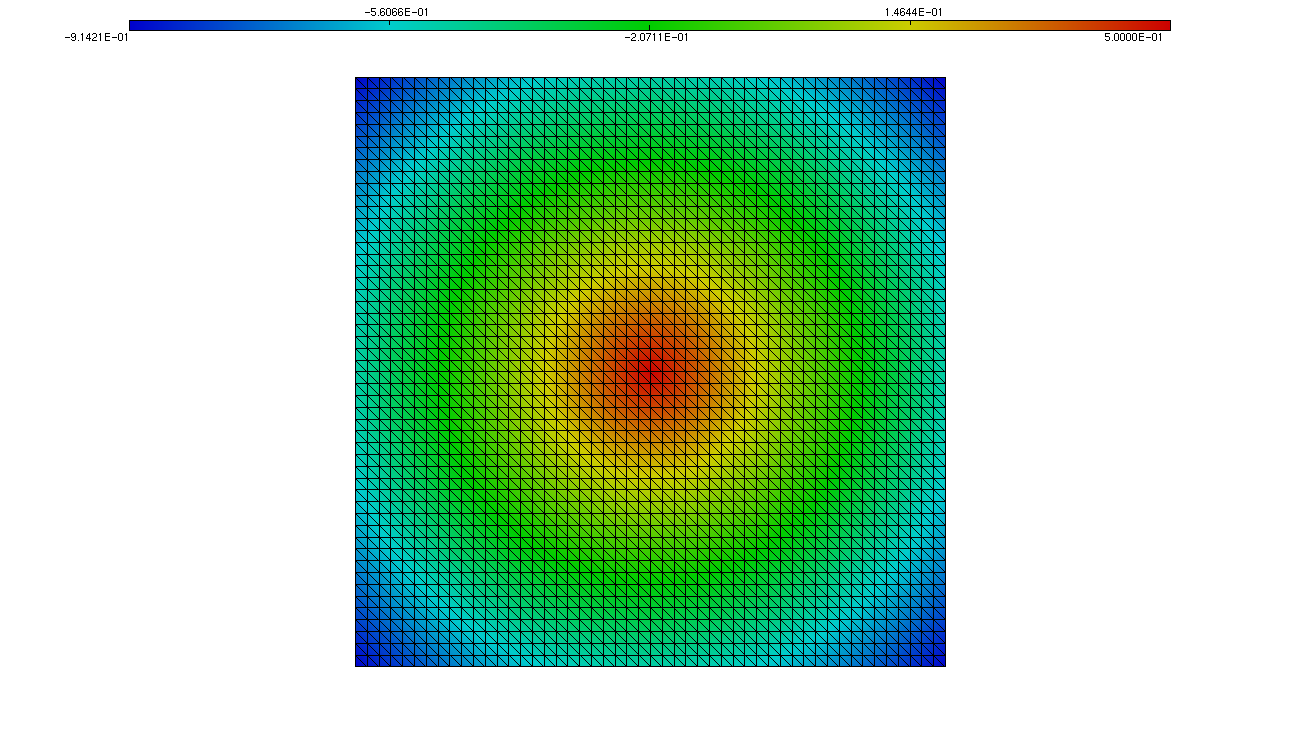
\includegraphics[clip=true, trim = 10cm 0 10cm 0, scale=.25]{Bordeaux/figures/LSinit.png}
		\captionof{subfigure}{Fonction Level Set représentée sur le maillage initial}
	\end{minipage}
	\hfill
	\begin{minipage}[t]{.5\linewidth}
		\centering
		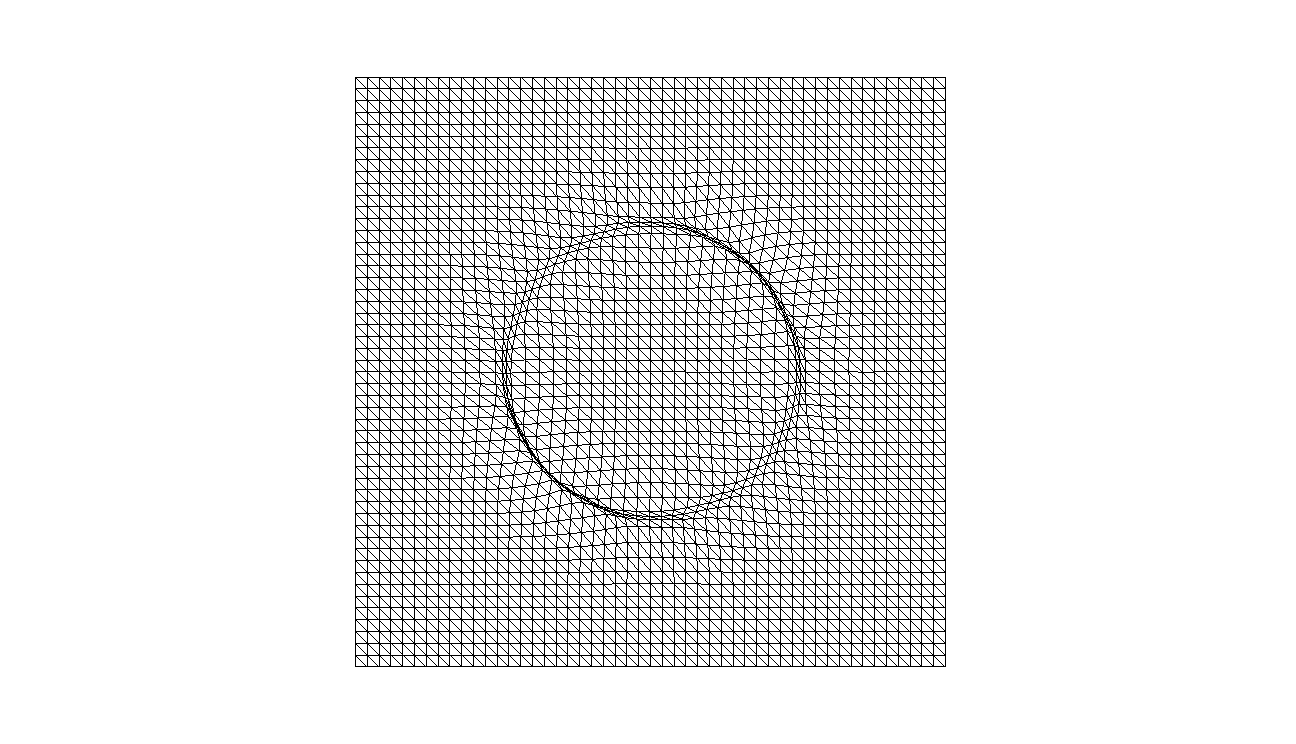
\includegraphics[clip=true, trim = 10cm 0 10cm 0, scale=.25]{Bordeaux/figures/LSadapt.png}
		\captionof{subfigure}{Maillage adapté à la fonction Level Set}
	\end{minipage}
	\captionof{figure}{Exemple d'adaptation à la fonction Level Set \label{fig:exLS}}
\endgroup

\subsection{Construction de la fonction à adapter (avec \(\omega\) donné par l'expression \eqref{eq:omega2})}

\indent Le calcul de \(\omega\) à partir de l'expression \eqref{eq:omega2} est fait en utilisant le gradient et le hessien de la fonction à adapter. Pourtant, dans le cas de la fonction Level Set, l'adaptation ne sera pas faite en considérant \(u=LS\), parce qu'on n'aurait pas de forts gradients, en tenant compte de la lisseté de cette fonction. Ainsi, \(\omega\) ne serait pas capable d'exprimer le raffinement désiré dans chaque partie du maillage. De cette façon, à partir de la fonction Level Set, on va construire une nouvelle fonction qui ait un très fort gradient sur les bords de l'objet.

\indent Idéalement, on construirait une fonction avec un saut, valant \(1\) à l'extérieur et \(-1\) à l'extérieur de l'objet, ce que fournit des très bons raffinements sur la ligne de niveau 0 de la fonction Level Set. Néanmoins, dans la résolution numérique de problèmes de la mécanique des fluides, il est intéressant d'avoir aussi un bon raffinement du maillage sur une couche autour de la surface (la couche limite de l'écoulement), où l'interaction fluide-objet n'est pas négligeable. En effet, pour avoir un calcul précis, un maillage approprié sur la couche limite est requis par la plupart des schémas numériques et logiciels pour les problèmes de fluides \cite{loseille}. Ainsi, on a cherché une fonction plus lisse.

\indent Dans un premier moment, on a défini une fonction avec une variation linéaire entre les deux étages (figure \ref{fig:atan}). Néanmoins, les tests réalisées ont fourni des résultats de mauvaise qualité : étant le gradient constant à l'intérieur de la pente, les points dans cette région (y compris les points les proches du bord de l'objet) n'avaient pas la tendance de bouger, au contraire des points proches des bordes de la pente, dû à la discontinuité du gradient de \(u\). Par conséquent, l'adaptation produisait une maillage avec deux petites couches raffinées, qui ne représentaient pas la surface de l'objet (figure \ref{fig:LSlin}).

\begingroup
  \centering
  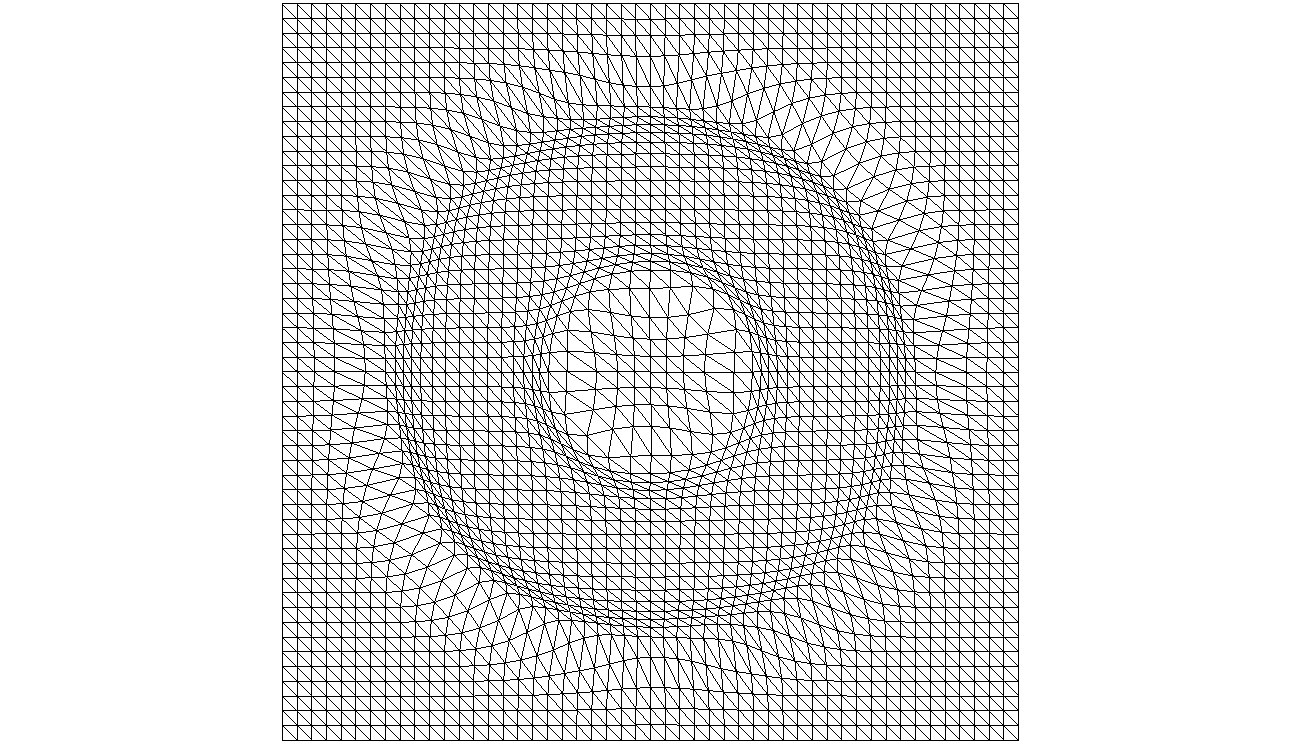
\includegraphics[clip=true, trim = 10cm 0 10cm 0, scale=.25]{Bordeaux/figures/LSlin.png}
  \captionof{figure}{Adaptation à une fonction Level Set modifié avec une variation linéaire \label{fig:LSlin}}
\endgroup

\indent On a ainsi cherché une fonction dont le gradient est plus variable et continue afin de réduire cet effet. On a obtenu des bons résultats en utilisant

\begin{equation}
	\label{eq:atan}
	u(\vecx) = \frac{1}{1.1.107} atan \left(\frac{2LS(\vecx)}{\delta} \right)
\end{equation}

\noindent étant \(2\delta\) la taille de la couche, choisie par l'utilisateur. Cette fonction est représentée dans la figure \ref{fig:atan}.

\begingroup
  \centering
  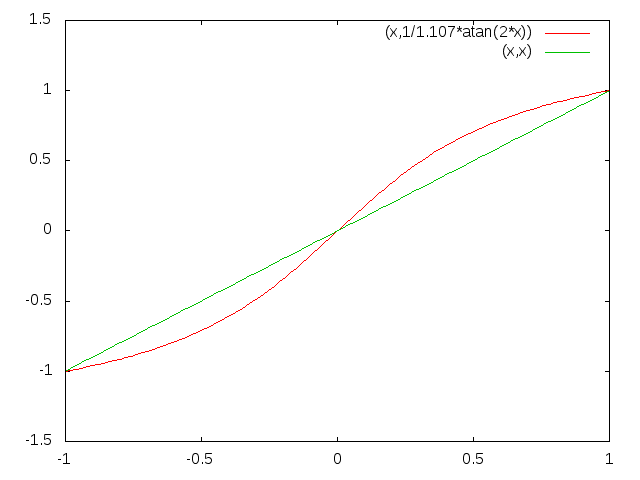
\includegraphics[scale=.4]{Bordeaux/figures/atan.png}
  \captionof{figure}{Comparaison des options pour la lissage de la fonction à adapter   \label{fig:atan}}
\endgroup

\indent On peut jouer aussi avec le paramètre multiplicateur de \(LS(\vecx)/\delta\) à l'intérieur de la fonction tangent. Avec 1, par exemple, on obtient un résultat plus proche de la pente linéaire; avec 5 ou 10, la fonction devient plus discontinue et la couche de raffinement est plus petite. On restera ainsi avec l'option donnée par \eqref{eq:atan}.



\subsubsection{Choix des paramètres}

\indent Afin de chercher les paramètres qui génèrent le meilleur maillage, plusieurs tests on été réalisés : 

\begin{itemize}
	\item Cas test (objet cible): 
	\begin{itemize}
		\item Cercle;
		\item Triangle;
		\item Profil d'une aile (NACA)
	\end{itemize}
	\item Type de maillage
	\begin{itemize}
		\item Structuré;
		\item Non structuré
	\end{itemize}
\end{itemize}

\indent Les meilleurs maillages obtenus on été utilisés pour résoudre un problème d'écoulement autour de l'objet, afin de vérifier l'influence sur les résultats. Les conclusions des tests sont les suivants : 

\begin{itemize}
  \item Pour le calcul de \(\omega\), il faut plutôt utiliser le gradient de \(u\). Le hessien peut être aussi utilisé, mais il a la tendance de créer deux couches raffinées dans les bords de la région de variation de la fonction \(u\) (figure \ref{fig:alphabeta});
  \item Le raffinement d'une certaine région du maillage cause un étirement dans la direction normale à surface des éléments voisins à cette région. Ce résultat n'est pas désirable car on veut plutôt une anisotropie dans la direction de l'écoulement du fluide (figure \ref{fig:anisoNormal}) : l'erreur d'interpolation est plus petit si on a des triangles anisotropes dont le côté le plus long est dans la direction des petites dérivées de deuxième ordre de la solution \cite{rippa}. Ainsi, il est important de avoir une valeur de \(\delta\) assez grande.
  \item Néanmoins, \(\delta\) ne peut être trop grand, car la fonction arctangente s'approche de la pente linéaire, et on n'obtient pas un bon raffinement à l'intérieur de la couche.
\end{itemize}


\begingroup
	\begin{minipage}[t]{.5\linewidth}
		\centering
		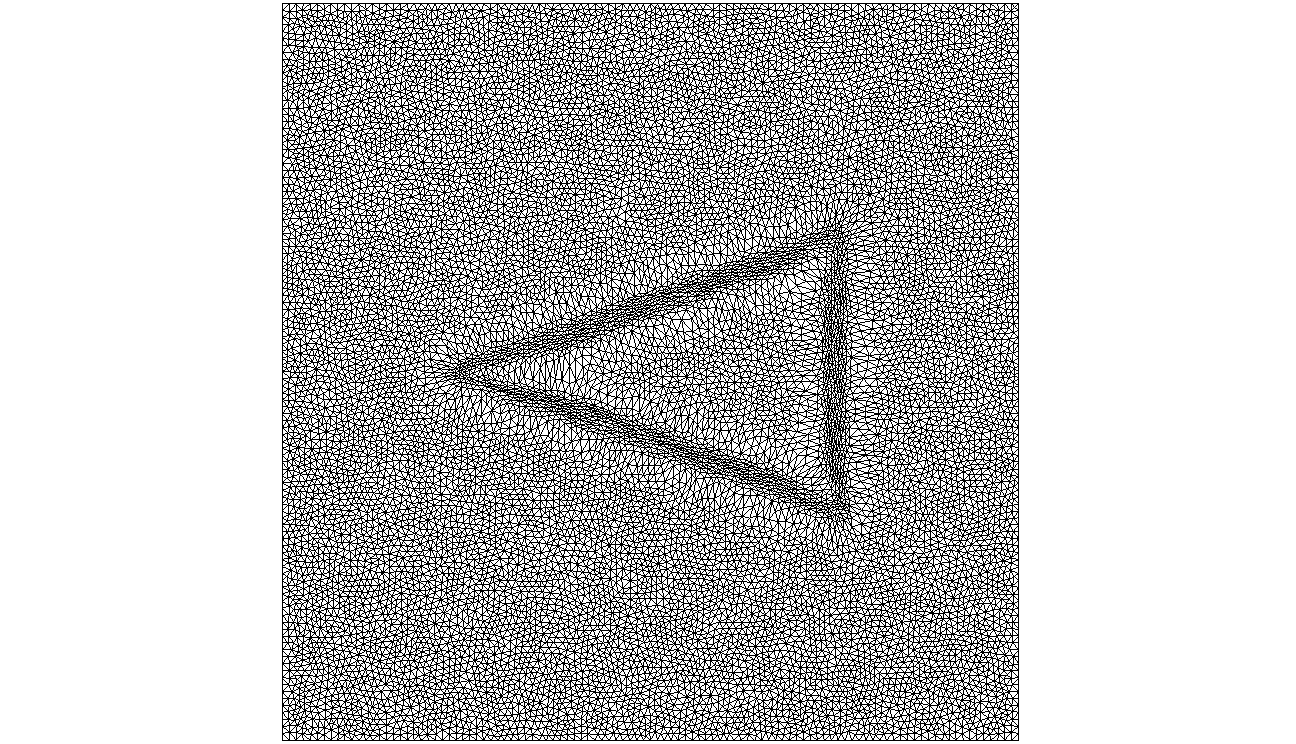
\includegraphics[clip=true, trim = 10cm 0 10cm 0, scale=.25]{Bordeaux/figures/alphabeta0.png}
		\captionof{subfigure}{\(\alpha = 1000, \beta = 0\)}
	\end{minipage}
	\hfill
	\begin{minipage}[t]{.5\linewidth}
		\centering
		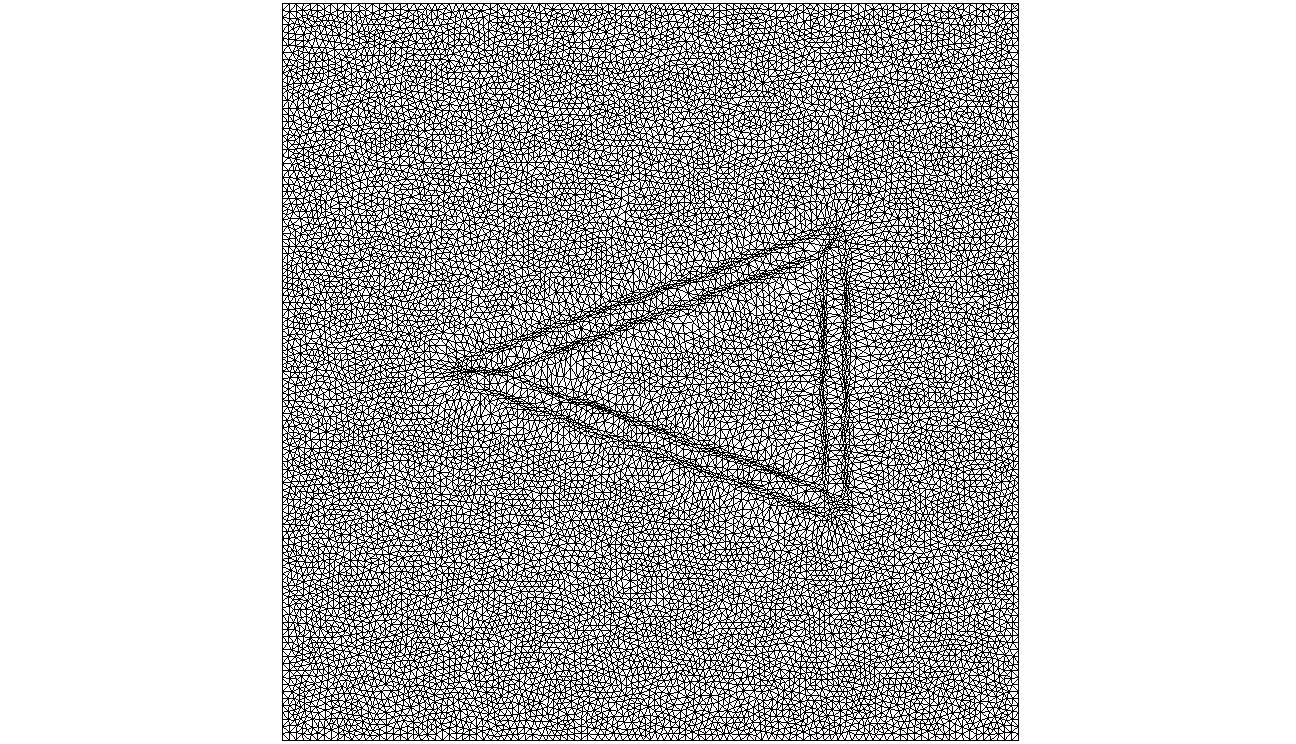
\includegraphics[clip=true, trim = 10cm 0 10cm 0, scale=.25]{Bordeaux/figures/alphabeta1.png}
		\captionof{subfigure}{\(\alpha = 0, \beta = 1000\)}
	\end{minipage}
	\captionof{figure}{Influence des paramètres \(\alpha\) et \(\beta\) sur l'adaptation du maillage (les deux cas ave \(\delta = 0.02\)) \label{fig:alphabeta}}
\endgroup

\begingroup
	\centering
	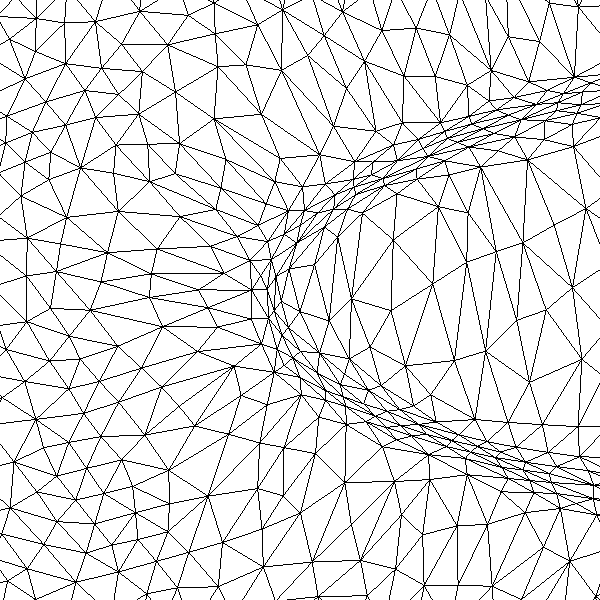
\includegraphics[scale=.25]{Bordeaux/figures/anisoNormal.png}
	\captionof{figure}{Détail d'un maillage obtenu avec \(\delta = 0.005\) \label{fig:anisoNormal}}
\endgroup

\indent En tenant compte de ces conclusions, on recommande l'utilisation des paramètres suivants (on rappelle qu'on utilise toujours les normes du gradient et du hessien normalisés entre 0 et 1) : 

\begin{equation*}
	\boldsymbol{\alpha} = 1000, \qquad 
	\boldsymbol{\beta} = 0, \qquad
	\boldsymbol{\delta} = 0.01,\  0.02
\end{equation*}

\indent On peut aussi faire des adaptations successives, en faisant varier les paramètres, afin d'obtenir d'autres résultats. Par exemple, on peut faire une première adaptation avec \(\delta = 0.02\) pour obtenir une bonne couche raffinée, et après une deuxième avec \(\delta = 0.01\) pour obtenir un raffinement plus précis autour de la surface. 

\indent La figure \ref{fig:example} présente quelques exemples d'adaptation à une fonction Level Set, avec les paramètres présentés ci-dessus, sur un maillage non structuré avec environ 28000 noeuds : 

\begingroup
	\begin{minipage}[t]{.5\linewidth}
    		\centering
		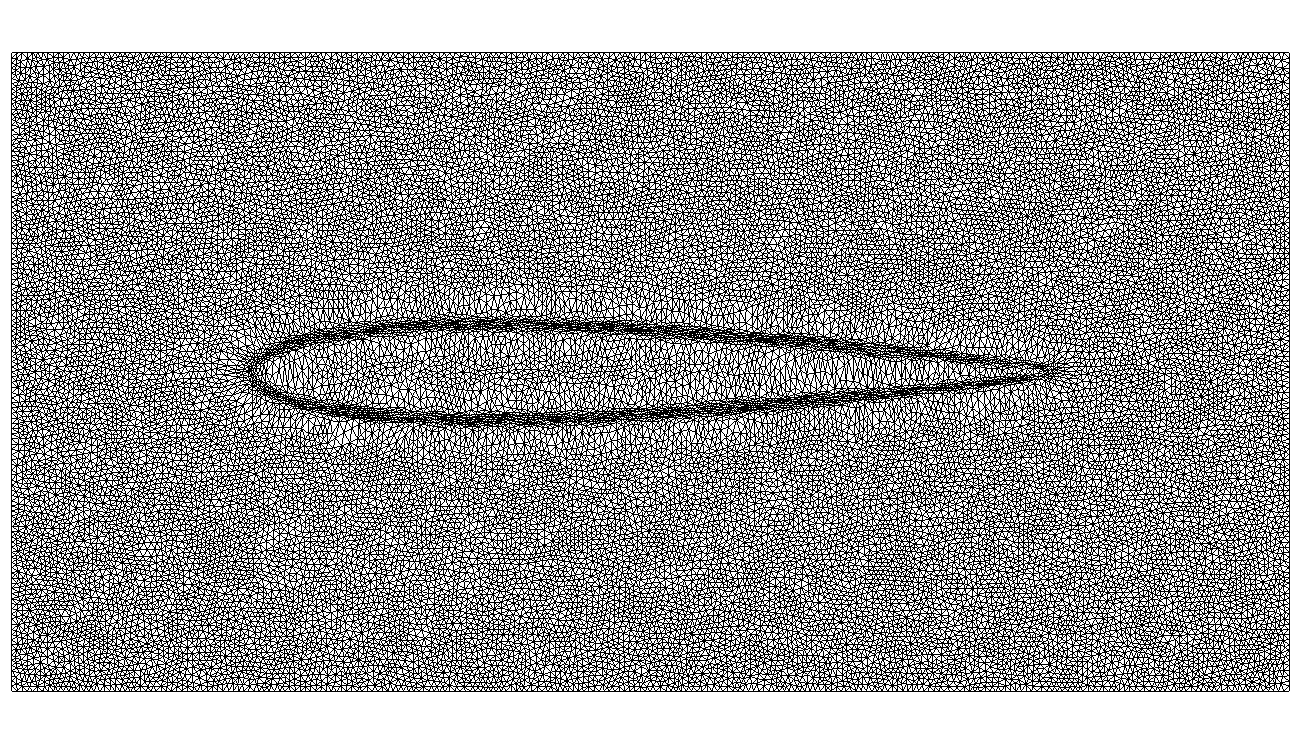
\includegraphics[scale=.15]{{Bordeaux/figures/example1}.png}
		\captionof{subfigure}{\(\delta = 0.01\)}
  	\end{minipage}
	\begin{minipage}[t]{.5\linewidth}
    		\centering
		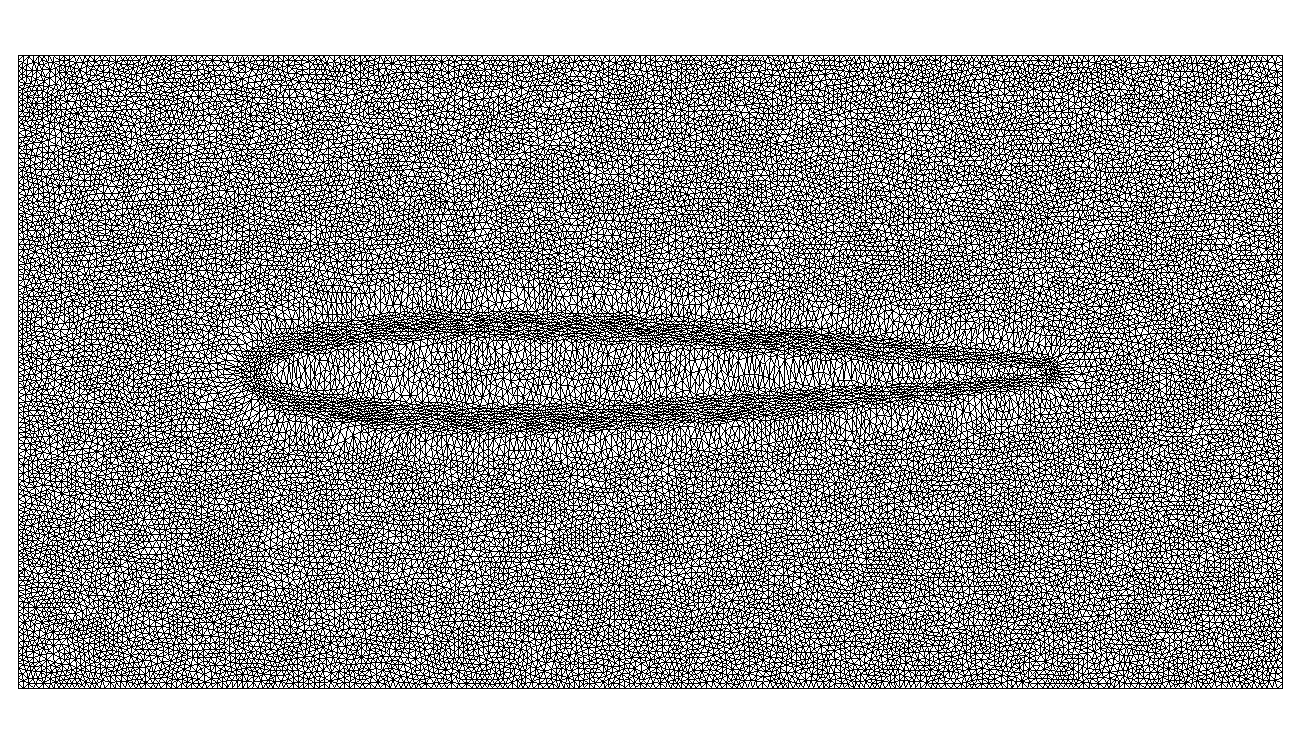
\includegraphics[scale=.15]{{Bordeaux/figures/example2}.png}
		\captionof{subfigure}{\(\delta = 0.02\)}
  	\end{minipage}
  	\captionof{figure}{Exemples d'adaptation à une fonction Level Set \label{fig:example}}
\endgroup


\subsection{Calcul des tailles désirées}

\indent Le calcul des tailles désirées est basée sur la définition d'une métrique pour chaque point du maillage. Il s'agit d'une matrice \(2 \times 2\) (dans le cas bidimensionnel) définie positive symétrique, construite de façon a contrôler l'erreur de la représentation de la solution sur le maillage modifiée \cite{leo}.


\indent La description détaillé de la définition, calcul et interprétation géométrique de la métrique seront faites dans la section \ref{sec:adapPhysique}, pour l'adaptation à une solution physique. Dans le cas de l'adaptation Level Set, on a implémenté un calcul simple des tailles désirées, en se basant sur la méthode utilisée par \cite{ducrot}, qui permet de contrôler la distance de Hausdorff entre la surface de l'objet et sa représentation. En faisant attention toujours à l'importance, pour une bonne adaptation,  de créer une fonction \(\omega\) qui soit au même temps assez lisse et qui présente des variations qui permettent le mouvement des noeuds, on définit, avec le paramètre \(\delta\), des couches pour l'imposition des tailles : 

\begin{equation*}
	\hdes (\vecx_i) =
	\begin{cases}
		\hm \ \ \ si \ \ |LS(\vecx_i)| \leq \frac{\delta}{2} \\
		2\hm \ \ \ si \ \ \frac{\delta}{2} \leq |LS(\vecx_i)|  \leq \delta \\
		\hM \ \ \ sinon
	\end{cases}
\end{equation*}

\noindent et on lisse les tailles sur le maillage avec le logiciel \emph{MMG}, en imposant une gradation de 10\%.

\subsubsection{Résultats}

\indent La figure \ref{fig:adaptMet} illustre l'adaptation Level Set basée sur l'imposition de tailles désirées à chaque noeud.

\begingroup
	\begin{minipage}[t]{.5\linewidth}
		\centering
		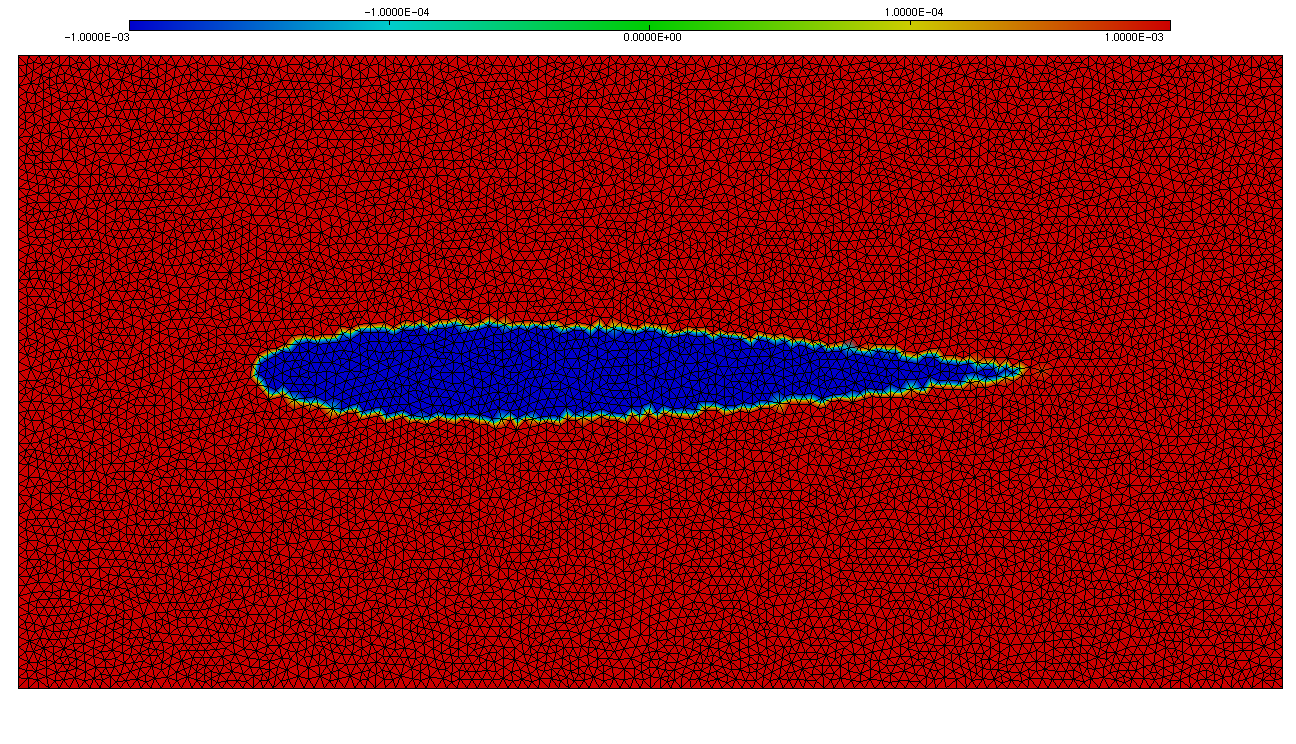
\includegraphics[scale=.15]{Bordeaux/figures/metLSNacaLS.png}
		\captionof{subfigure}{Fonction Level Set}
	\end{minipage}
	\hfill
	\begin{minipage}[t]{.5\linewidth}
		\centering
		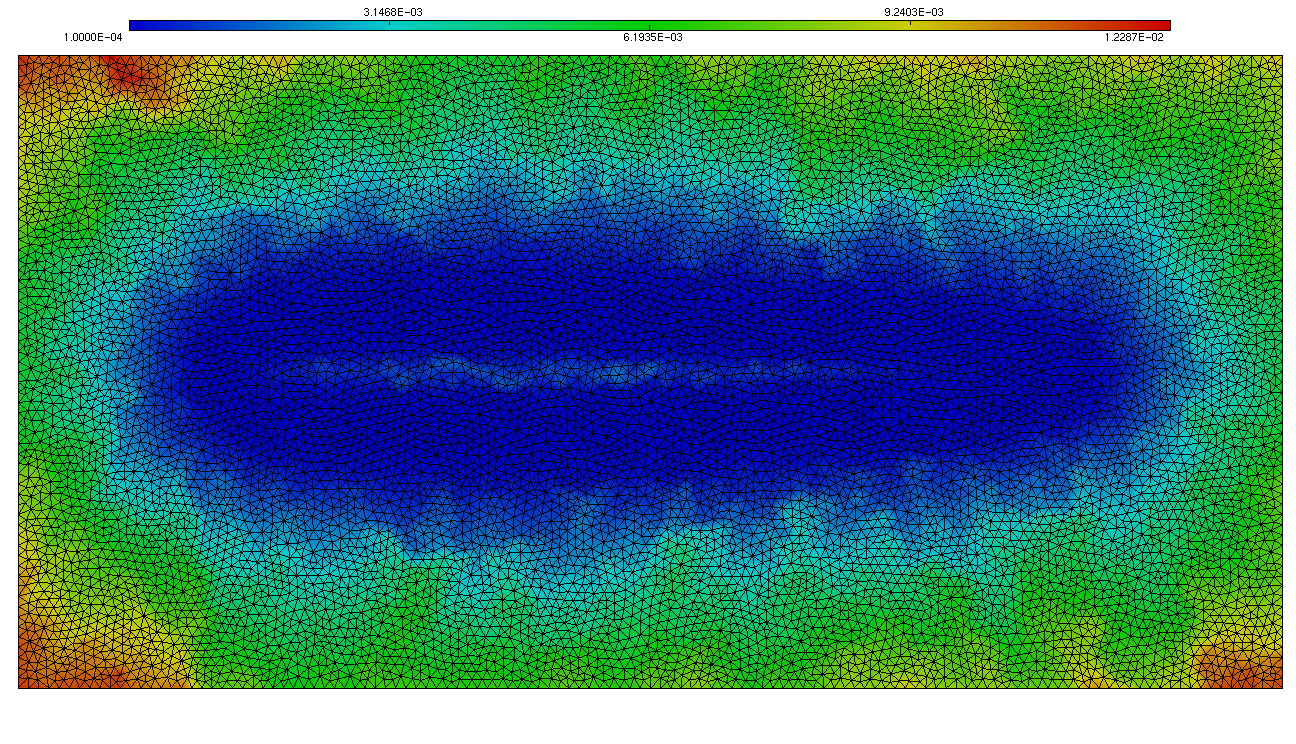
\includegraphics[scale=.15]{Bordeaux/figures/metLSNacaMet.png}
		\captionof{subfigure}{Tailles désirées}
	\end{minipage}	
	\begin{minipage}[t]{1.\linewidth}
		\centering
		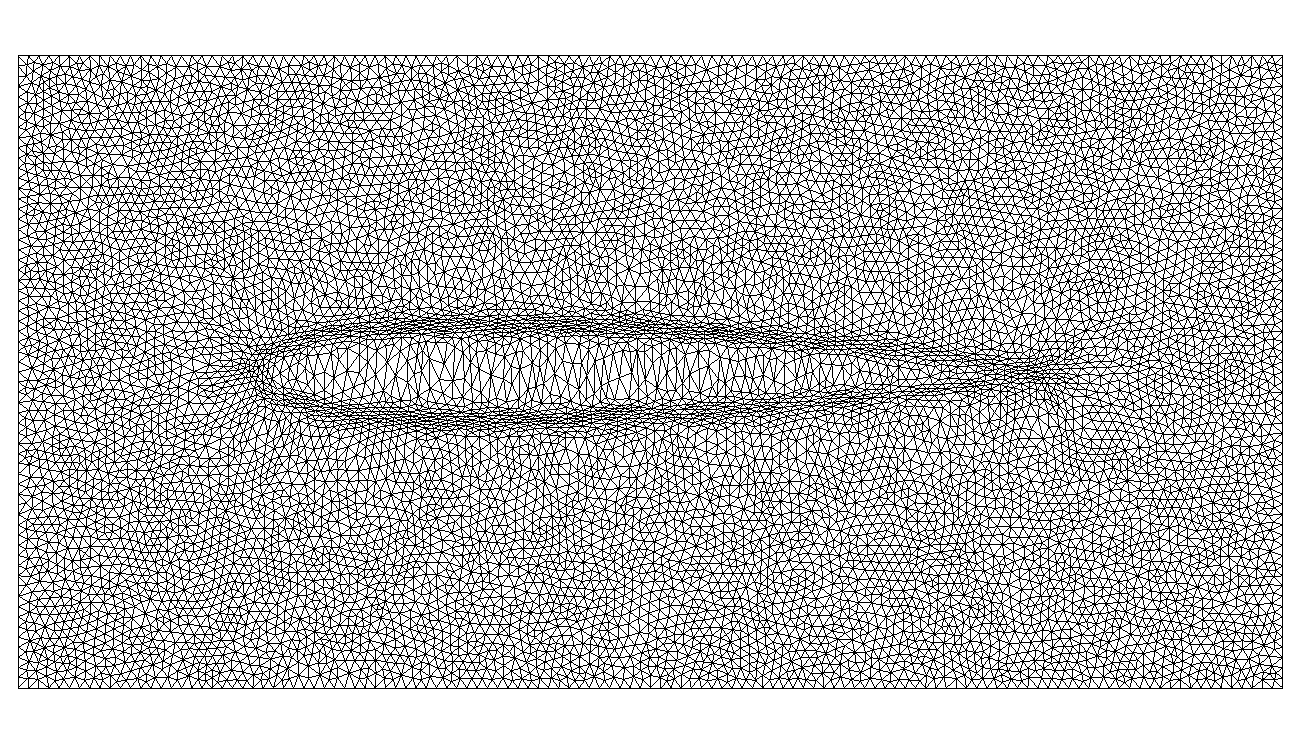
\includegraphics[scale=.2]{Bordeaux/figures/metLSNacaAdapt.png}
		\captionof{subfigure}{Maillage adapté (20 itérations)}
	\end{minipage}	
	\captionof{figure}{Adaptation à une fonction Level Set à partir de l'imposition des tailles désirées \label{fig:adaptMet}}
\endgroup


\subsection{Relaxation et qualité du maillage}

\indent Pendant la résolution du système linéaire, on fait, si nécessaire, une relaxation des déplacements calculés afin d'éviter le croisement des noeuds et la conséquente occurrence d'aires négatives. Néanmoins, en dépendant du maillage de départ (par exemple, un maillage déjà raffiné), la relaxation est trop contraignant et impose l'arrêt de l'algorithme lors des premières itérations. Parfois cela est provoqué par un petit nombre d'éléments.

\indent On a ainsi implémenté, dans les premières itérations, un prétraitement d'optimisation, selon le schéma suivant :

\begin{itemize}
  \item Si le numéro de l'itération actuelle n'est pas supérieur à \(iter_{optim}\) : 
  \begin{enumerate}
    \item Identifier tous les éléments qui demanderont de la relaxation;
    \item Classifier ces éléments selon un critère de qualité (mesure de l'anisotropie);
    \item Optimiser les \(n_{optim}\) éléments les plus critiques de cette liste
  \end{enumerate}   
\end{itemize}

\indent L'optimisation réalisée consiste en, itérativement, approcher chaque noeud \(i\) de l'élément concerné du barycentre des noeuds voisins de \(i\). L'optimisation est arrêtée dès qu'aucun des trois noeuds de l'élément bouge au dessus d'un seuil, ou qu'au moins un des noeuds n'arrive pas à réduire l'anisotropie au dessous d'une certaine pourcentage, par rapport au début de l'itération.

\indent La figure \ref{fig:optim} montre le résultat de son application sur un élément : 

\begingroup
	\begin{minipage}[t]{.5\linewidth}
    		\centering
		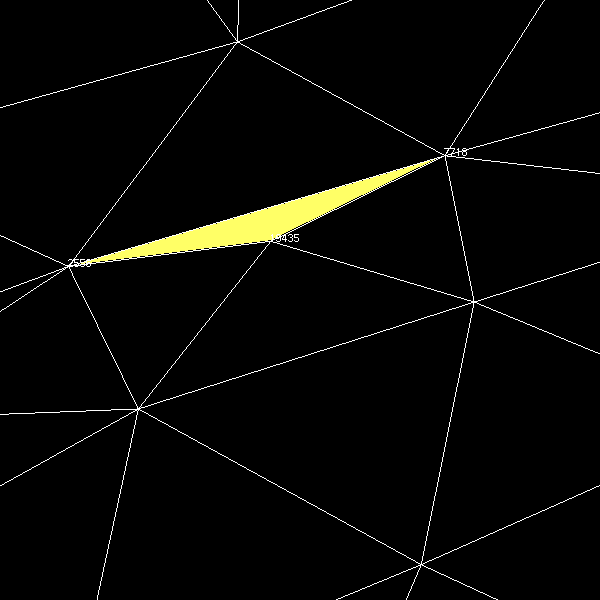
\includegraphics[scale=.25]{{Bordeaux/figures/optim_avant}.png}
		\captionof{subfigure}{Avant l'optimisation}
  	\end{minipage}
  	\hfill
	\begin{minipage}[t]{.5\linewidth}
    		\centering
		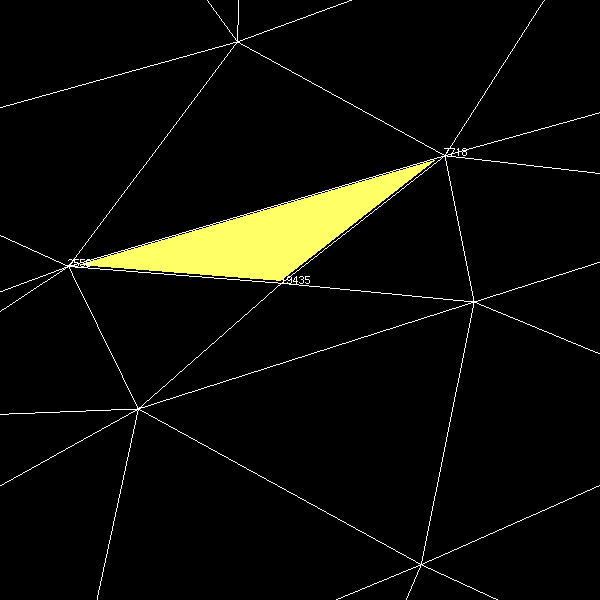
\includegraphics[scale=.25]{{Bordeaux/figures/optim_apres}.png}
		\captionof{subfigure}{Après l'optimisation}
  	\end{minipage}
  	\captionof{figure}{Résultat de l'optimisation d'un élément \label{fig:optim}}
\endgroup

\indent Pour que le prétraitement ne soit pas très coûteux, on a choisi \(n_{optim} = 10\) e \(iter_{optim} = 2\). Les tests réalisés montrent des très bons résultats quand l'algorithme s'arrête au début de l'exécution, et avec l'optimisation on arrive à tourner tous les itérations. Néanmoins, si appliqué sur un maillage de bonne qualité et qui ne demande pas une forte relaxation, les gains sont en général petits (ou même on perd un peu de la qualité du résultat final).


\subsection{Adaptation 3D}

\indent Après le développement et validation du modèle bidimensionnel décrit jusqu'ici, avec l'obtention de bons résultats d'adaptation des maillages, on l'a étendu au cas tridimensionnel. Du point de vue théorique, cette extension est assez simple, étant le modèle toujours décrit par le problème \eqref{eq:systeme}. Le développement de sa formulation faible reste aussi la même, et on se ramène ainsi à la résolution des systèmes linéaires

\begin{equation*}
	\begin{cases}
		Kx = 0 \\
		Ky = 0 \\
		Kz = 0
	\end{cases}
\end{equation*}

\indent Comme ces systèmes sont indépendants et ont la même forme, l'extension du cas 2D au 3D a été également simple du point de vue de l'implémentation. En effet, parmi les calculs décrits en détail dans les sous-sections \ref{subsec:calculK} et \ref{subsec:jacobi}, l'unique modification concerne le calcul des vecteurs normaux (\((\nabref \phii)^T = \frac{\normT{i}}{d!|T|}\), avec \(d=3\)). Ainsi, les éléments de la matrice \(K\) sont donnés par


\begin{equation*}
\begin{gathered}
\begin{aligned}
	k_{ij} & = \iDomh{ \omega \nabref \phii  \cdot \nabref \phij } = \sum_{T \ni i} {\iT{ \omega \nabref \phii \cdot \nabref \phij }} = \\
	       &  = \sum_{T \ni i}
	              { 
	                     { |T|\omega^T \frac{\normT{i}\cdot \normT{j}}{(3!|T|)^2}
	                     }
	              }
	          = \sum_{T \ni i}
	              { 
	                     { \omega^T \frac{\normT{i}\cdot \normT{j}}{36|T|}
	                     }
	              }	              
\end{aligned}
\end{gathered}
\end{equation*}

\indent On présente dans les figures \ref{fig:adaptSphere} à \ref{fig:adaptHole} quelques résultats de l'adaptation Level Set tridimensionnelle, à partir de l'imposition des tailles désirées. Les fonctions Level Set utilisées sont celles de la figure \ref{fig:LS}. Malgré les résultats analogues au cas 2D et cohérents avec les objectifs ici proposés, l'adaptation 3D a des limitations plus fortes concernant le nombre de points du maillage, qui peut devenir très grande pour qu'on ait un maillage suffisamment fine pour la bonne représentation de la fonction Level Set, et la relaxation de l'adaptation, puisque le dégrée de liberté additionnel peut conduire plus rapidement au croisement des noeuds.

\indent Les domaines de départ sont plus raffinées dans les régions où se trouve l'objet, afin de minimiser l'influence des bords sur l'adaptation. Le logiciel \emph{MMG} a été utilisé pour les générer, en imposant une taille minimale \(hmin =  0.05\) et une gradation de \(hgrad = 1.1\) de la variation de las tailles. Les adaptations ont été faites avec \(\delta\) entre 0.05 et 0.07.

\begingroup
	\begin{minipage}{.3\linewidth}
		\centering
		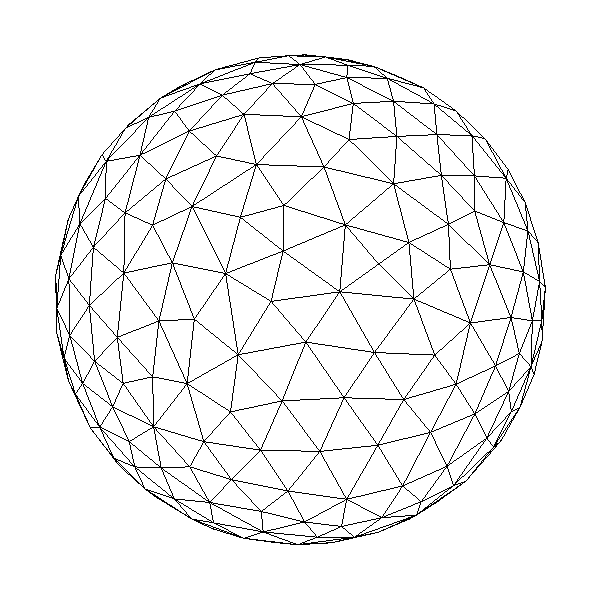
\includegraphics[scale=.2]{Bordeaux/figures/3D/sphereLS.png}
		\captionof{subfigure}{Sphere \label{fig:sphereLS}}
	\end{minipage}
	\hfill
	\begin{minipage}{.3\linewidth}
		\centering
		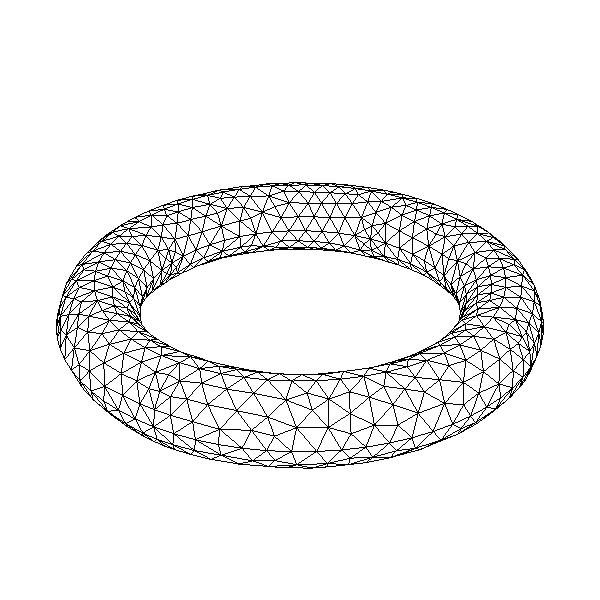
\includegraphics[scale=.2]{Bordeaux/figures/3D/torusLS.png}
		\captionof{subfigure}{Tore \label{fig:torusLS}}
	\end{minipage}
	\hfill
	\begin{minipage}{.3\linewidth}
		\centering
		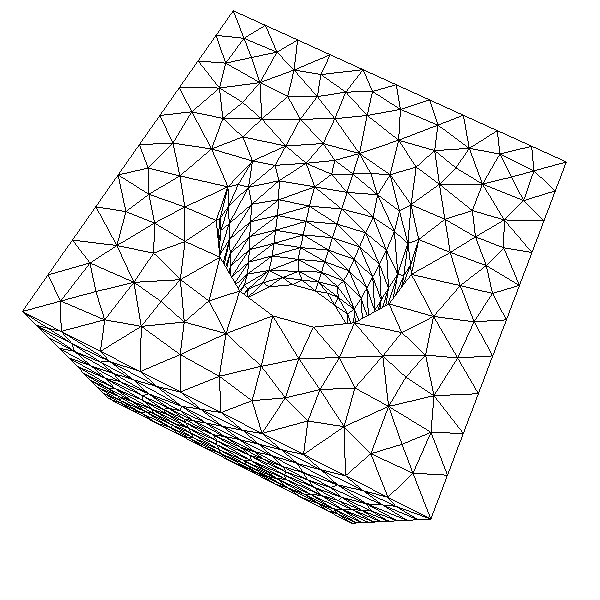
\includegraphics[scale=.2]{Bordeaux/figures/3D/holeLS.png}
		\captionof{subfigure}{Boîte avec un trou \label{fig:holeLS}}
	\end{minipage}
	\captionof{figure}{Fonctions Level Set utilisées \label{fig:LS}}
\endgroup

\begingroup
	\begin{minipage}[t]{.5\linewidth}
		\centering
		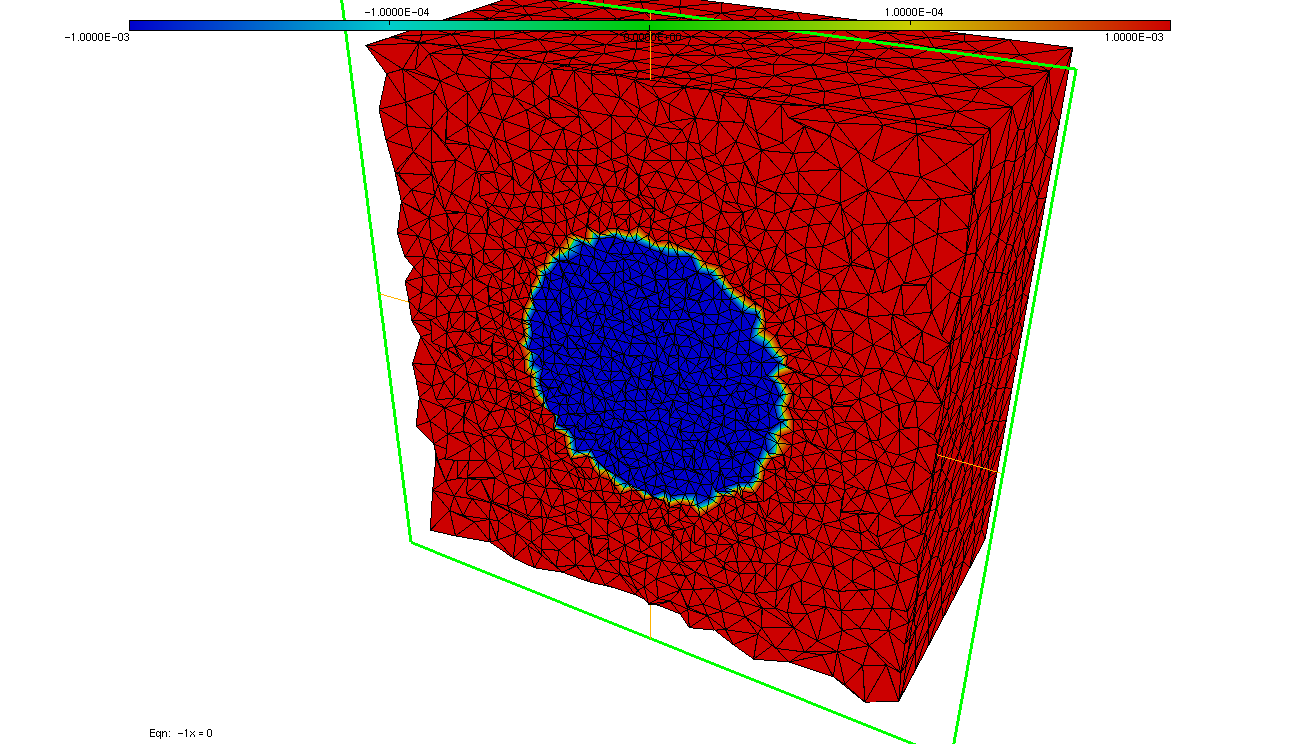
\includegraphics[clip=true, trim=5cm 0 2cm 0, scale=.2]{Bordeaux/figures/3D/sphereDomLS.png}
		\captionof{subfigure}{Fonction Level Set}
	\end{minipage}
	\hfill
	\begin{minipage}[t]{.5\linewidth}
		\centering
		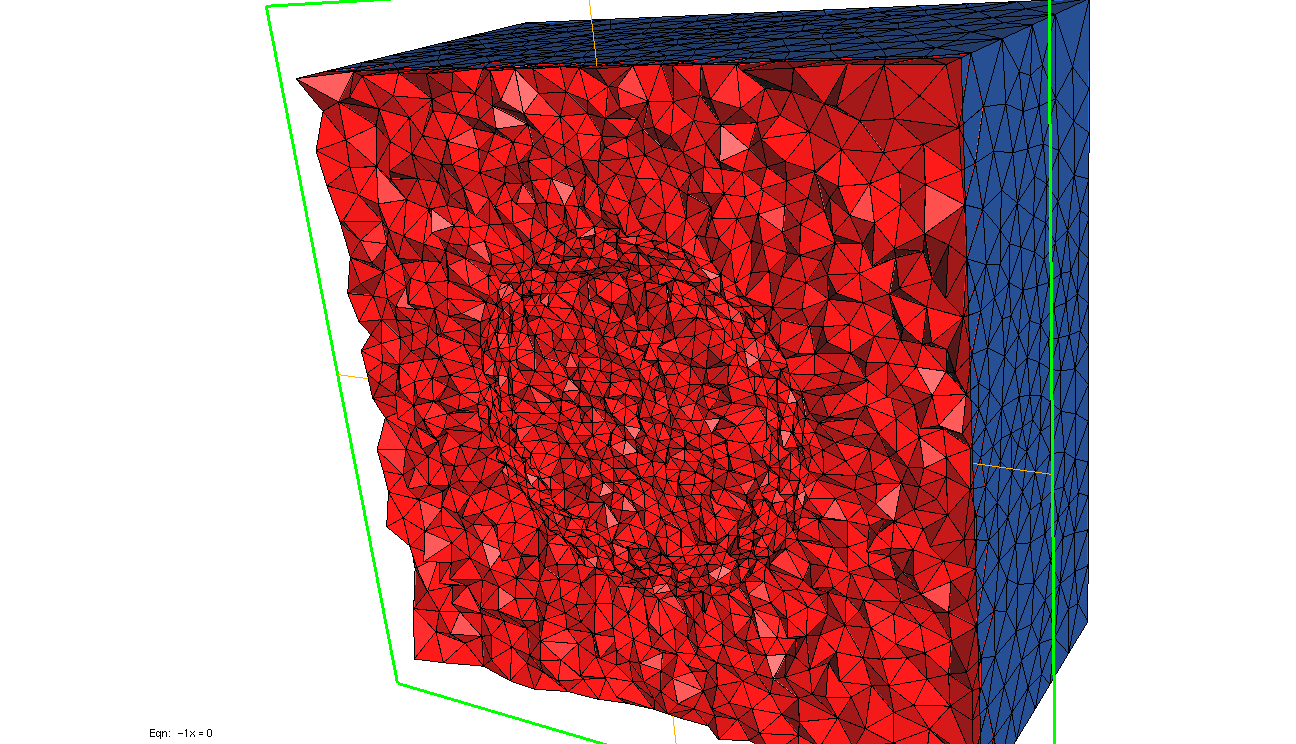
\includegraphics[clip=true, trim=5cm 0 5cm 0, scale=.2]{Bordeaux/figures/3D/sphereAdapt.png}
		\captionof{subfigure}{Maillage adapté (7 itérations)}
	\end{minipage}
	\captionof{figure}{Adaptation du maillage à la sphère (environ 34000 noeuds) \label{fig:adaptSphere}}
\endgroup

\begingroup
	\begin{minipage}[t]{.5\linewidth}
		\centering
		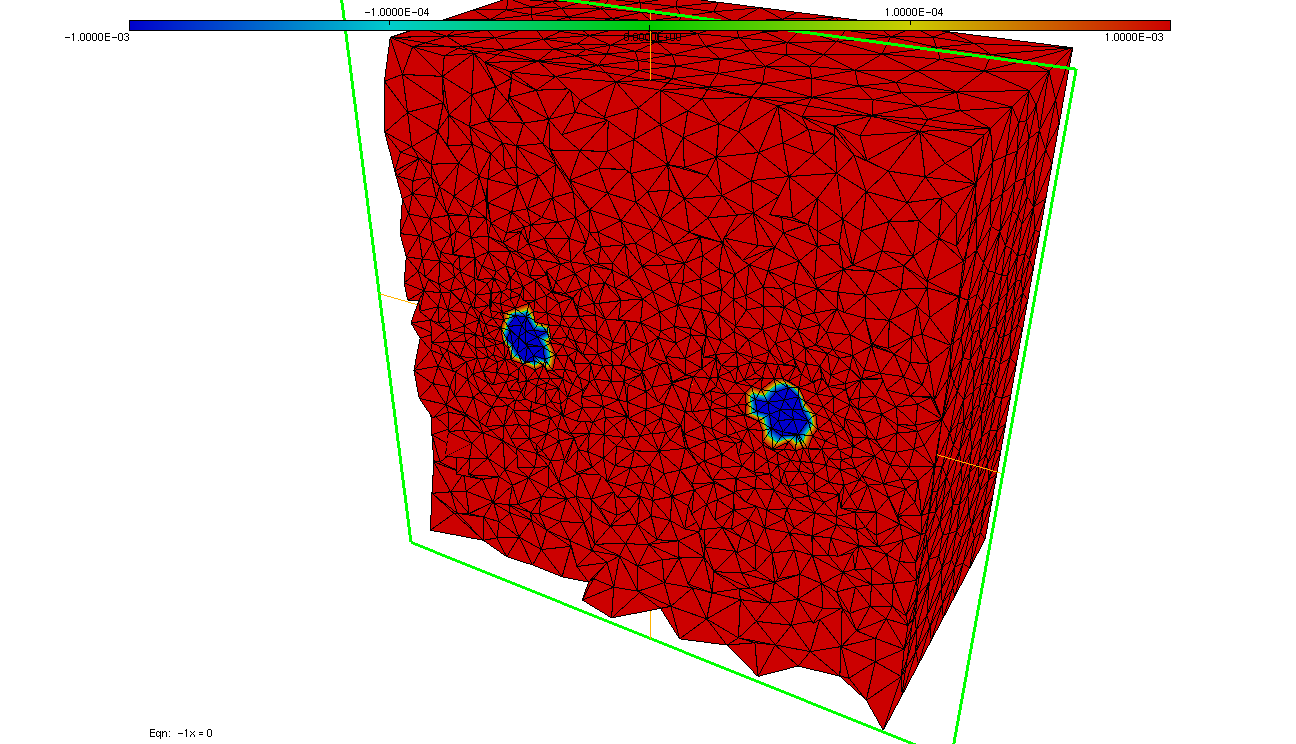
\includegraphics[clip=true, trim=5cm 0 2cm 0, scale=.2]{Bordeaux/figures/3D/torusDomLS1.png}
		\captionof{subfigure}{Fonction Level Set}
	\end{minipage}
	\hfill
	\begin{minipage}[t]{.5\linewidth}
		\centering
		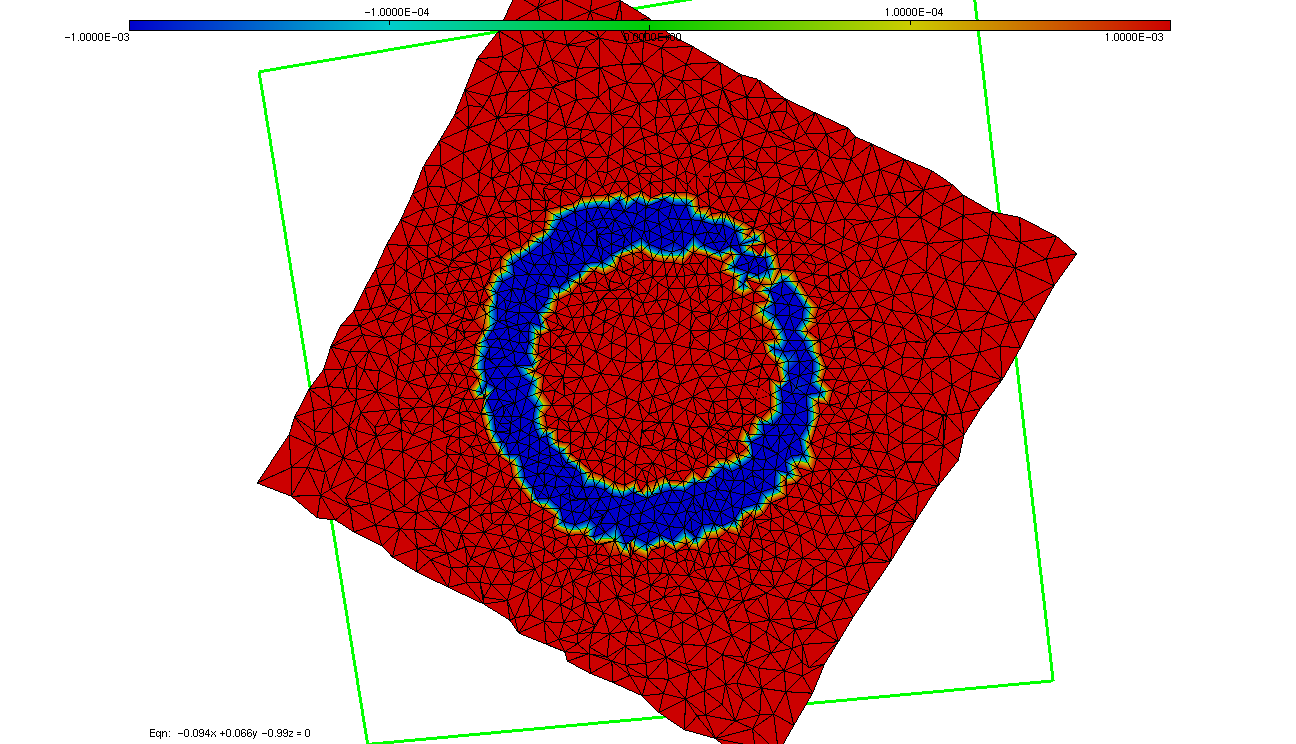
\includegraphics[clip=true, trim=5cm 0 2cm 0, scale=.2]{Bordeaux/figures/3D/torusDomLS2.png}
		\captionof{subfigure}{Fonction Level Set}
	\end{minipage}
	\begin{minipage}[t]{.5\linewidth}
		\centering
		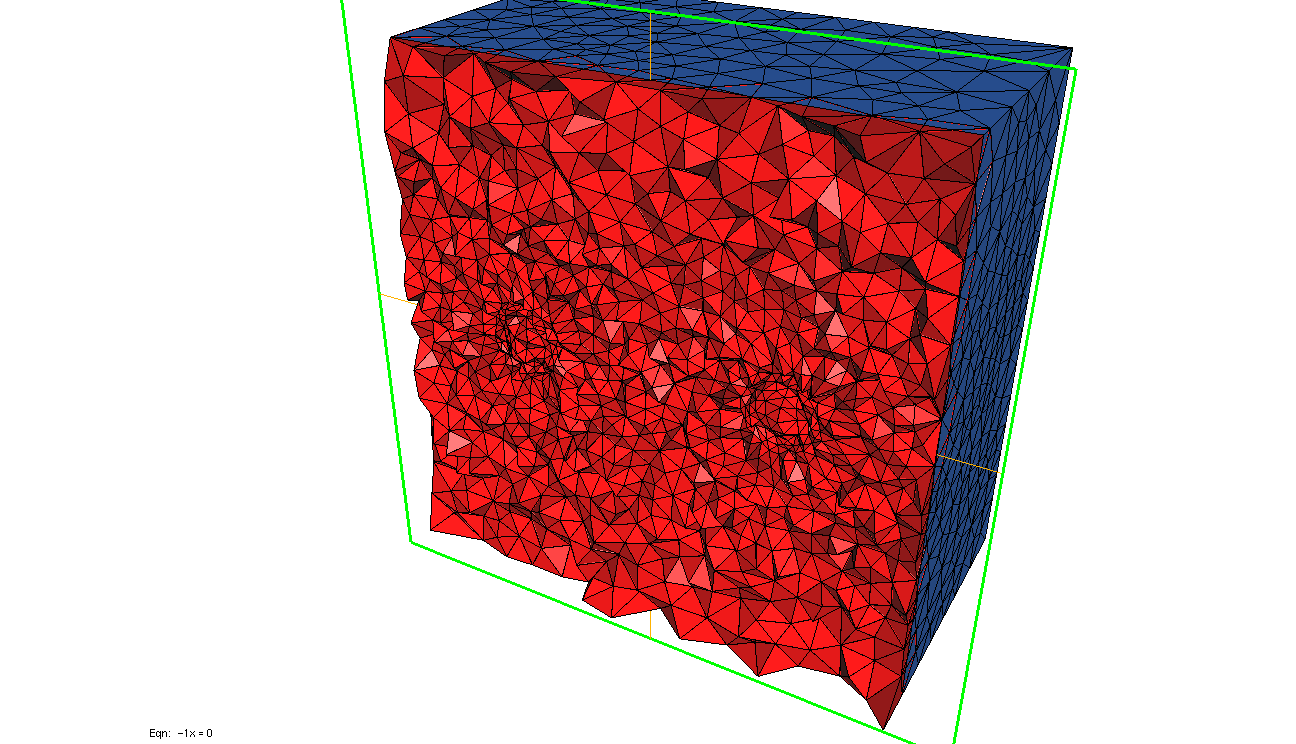
\includegraphics[clip=true, trim=5cm 0 2cm 0, scale=.2]{Bordeaux/figures/3D/torusAdapt2.png}
		\captionof{subfigure}{Maillage adapté (8 itérations)}
	\end{minipage}
	\hfill
	\begin{minipage}[t]{.5\linewidth}
		\centering
		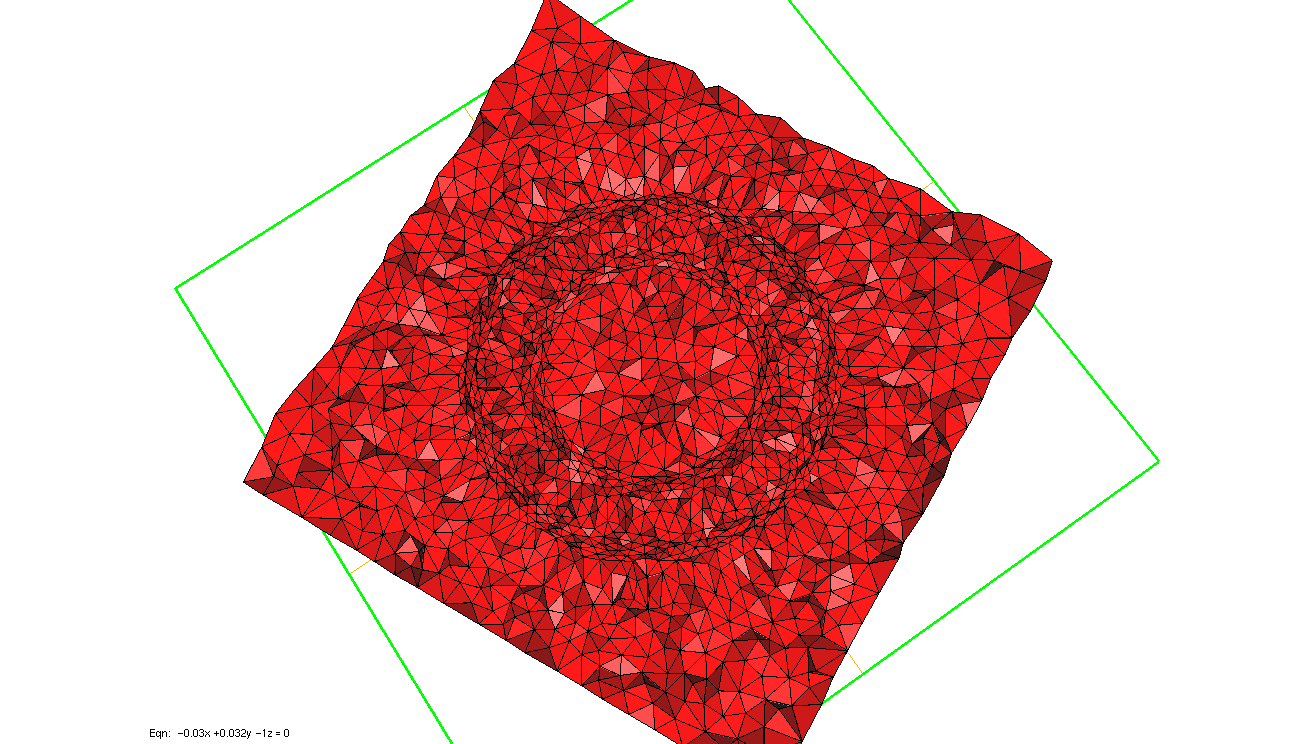
\includegraphics[clip=true, trim=5cm 0 2cm 0, scale=.2]{Bordeaux/figures/3D/torusAdapt1.png}
		\captionof{subfigure}{Maillage adapté (8 itérations)}
	\end{minipage}
	\captionof{figure}{Adaptation du maillage au tore (environ 25000 noeuds) \label{fig:adaptTorus}}
\endgroup

\begingroup
	\begin{minipage}[t]{.5\linewidth}
		\centering
		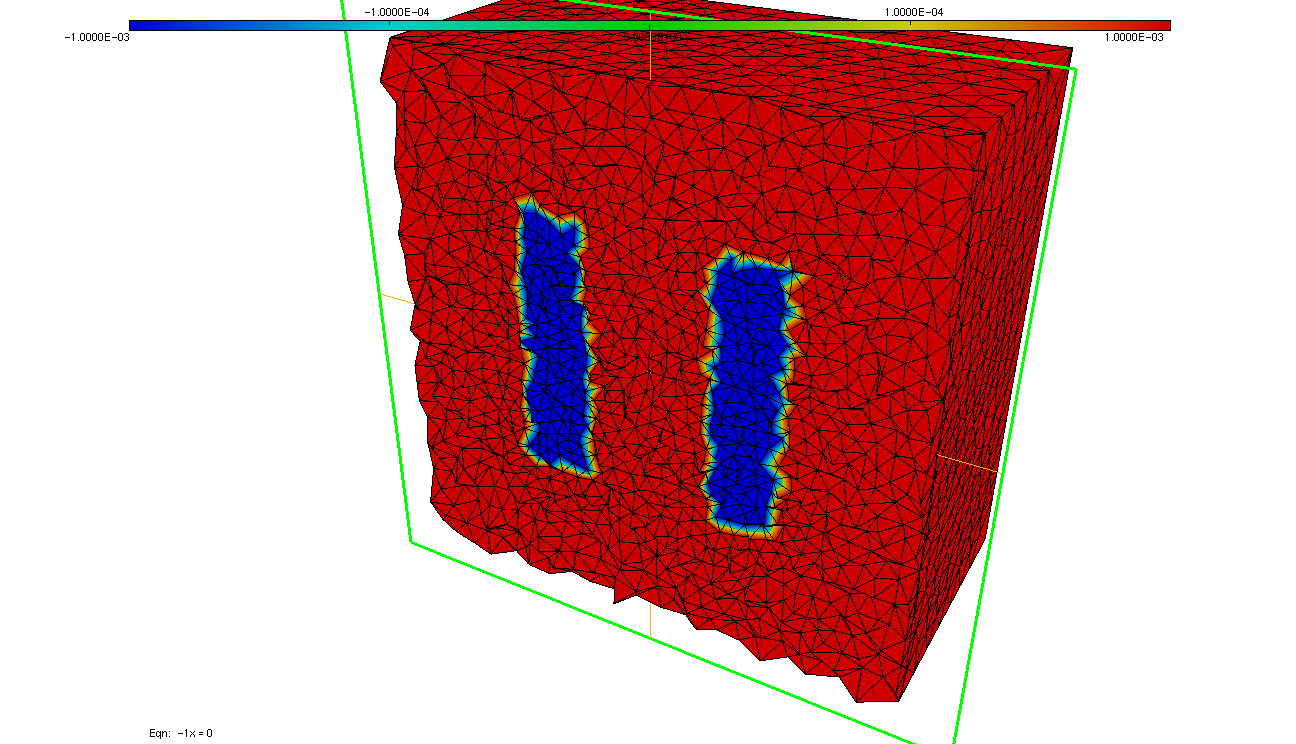
\includegraphics[clip=true, trim=5cm 0 2cm 0, scale=.2]{Bordeaux/figures/3D/holeDomLS1.png}
		\captionof{subfigure}{Fonction Level Set}
	\end{minipage}
	\begin{minipage}[t]{.5\linewidth}
		\centering
		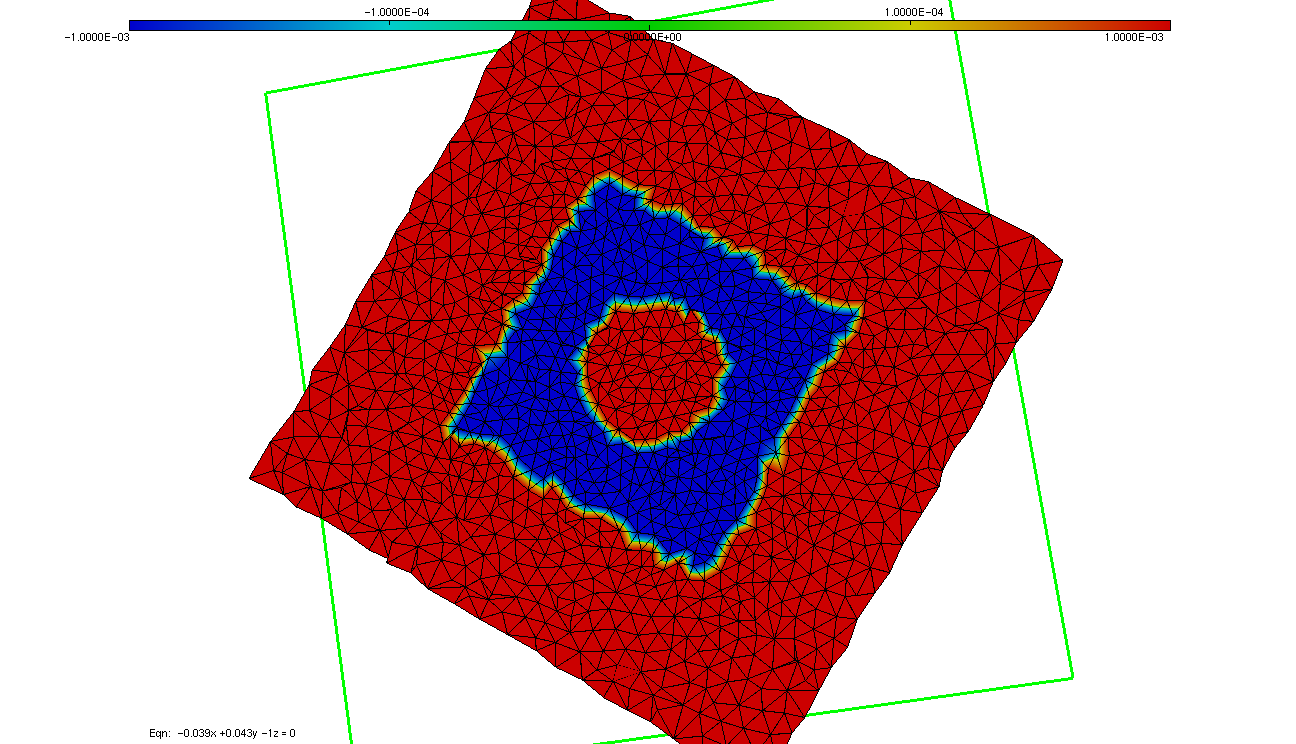
\includegraphics[clip=true, trim=5cm 0 2cm 0, scale=.2]{Bordeaux/figures/3D/holeDomLS2.png}
		\captionof{subfigure}{Fonction Level Set}
	\end{minipage}
	\begin{minipage}[t]{.5\linewidth}
		\centering
		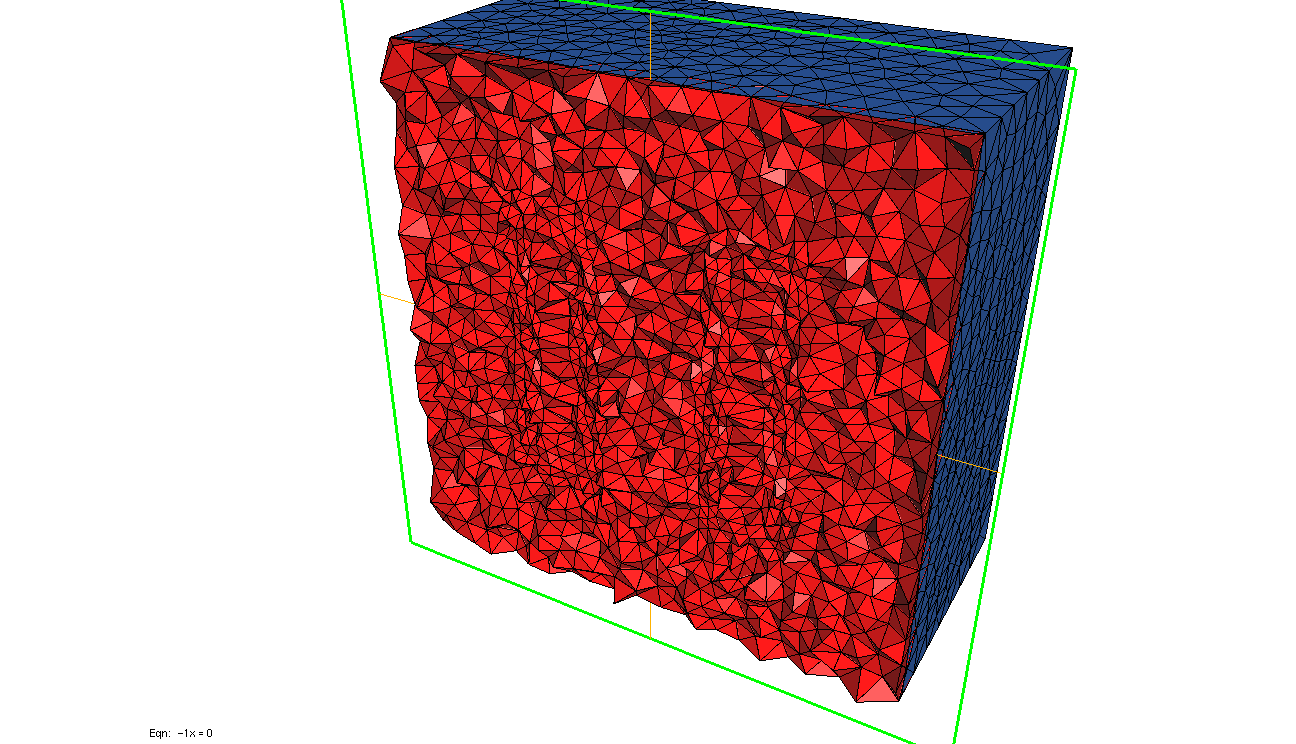
\includegraphics[clip=true, trim=5cm 0 2cm 0, scale=.2]{Bordeaux/figures/3D/holeAdapt1.png}
		\captionof{subfigure}{Maillage adapté (5 itérations)}
	\end{minipage}
	\begin{minipage}[t]{.5\linewidth}
		\centering
		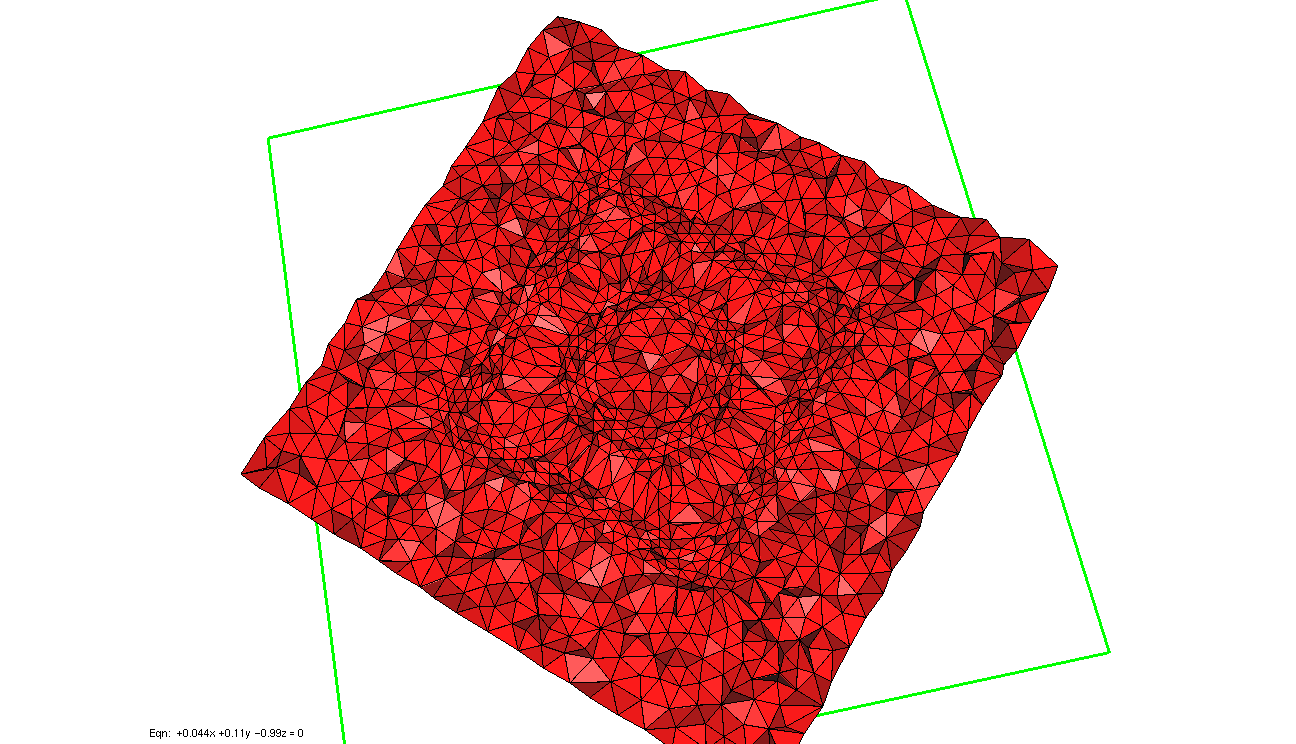
\includegraphics[clip=true, trim=5cm 0 2cm 0, scale=.2]{Bordeaux/figures/3D/holeAdapt2.png}
		\captionof{subfigure}{Maillage adapté (5 itérations)}
	\end{minipage}
	\captionof{figure}{Adaptation du maillage à une boîte avec un trou (environ 34000 noeuds) \label{fig:adaptHole}}
\endgroup
 \section{Application à l'adaptation physique}
\label{sec:adapPhysique}

\indent De la même façon que l'adaptation Level Set, l'adaptation physique (\emph{i.e.}, à une variable physique calculée sur le maillage, comme le champs de vitesse de l'écoulement) peut être faite avec les deux formulations de \(\omega\). Pour la première, basée sur la variation de la fonction, on n'a pas de remarques supplémentaires à faire : au contraire de la fonction Level Set, qui est toujours lisse, les variables physiques dans les problèmes de mécanique de fluides qui nous intéressent présentent en général des discontinuités, ayant ainsi des fortes gradients et hessiens qui permettent une bonne adaptation. Alors, il ne faut pas construire une autre fonction à adapter. 

\indent Ainsi, on détaille seulement le deuxième calcul de \(\omega\) :

\subsection{Calcul des tailles désirées}

\indent Le calcul des tailles présenté dans la suite s'inspire dans \cite{cecile_these} et \cite{frey_alauzet}, et s'est basée sur la notion de métrique : pour chaque noued \(i\) du maillage, on définit une matrice \(\met_i \ 2 \times 2\) (dans le cas bidimensionnel) qui minimise un estimateur de l'erreur d'interpolation de la solution sur le maillage.

\indent Étant \(\Pi_hu\) l'interpolation de \(u\) sur le maillage, cet estimateur est donné, pour chaque élément \(K\) du maillage, par

\begin{equation}
	\label{eq:erreur_interp}
	||u-\Pi_hu||_{\infty,K} \leq c_d \max_{x \in K}{\max_{\vec{e} \in E_K}{\langle \vec{e}, |H_u(\vecx)| \vec{e} \rangle}}
\end{equation}

\noindent où \(c_d = 2/9 \) est obtenu avec un développement de Taylor de \eqref{eq:erreur_interp} dans son point de maximum, et $E_K$ est l'ensemble des arêtes de $K$. On veut imposer une  limite \(\epsilon\) à cette erreur : 

\begin{equation*}
	||u-\Pi_hu||_{\infty,K} = \epsilon
\end{equation*}

\indent En définissant la métrique

\begin{equation}
	\label{eq:def_metrique}
	\met = \frac{c_d}{\epsilon}H_u(\vecx)
\end{equation}

\noindent la longueur des arêtes selon cette métrique est alors

\begin{equation*}
	l_{\met_i} = \langle \vec{e}, |\met_i| \vec{e} \rangle = 1
\end{equation*}

\noindent c'est à dire, la métrique qui assure l'erreur d'interpolation désirée est celle telle que le maillage soit unitaire \cite{cecile_these,frey_alauzet}.

\indent Étant la métrique une matrice positive définie symétrique, elle est toujours diagonalisable es ses valeurs propres \(\tilde{\lambda}_i^j, j=1,2\), sont toujours réelles. En effet, la métrique peut être représentée par une ellipse (ou un ellipsoïde, en 3D), dont les vecteurs propres donnent la direction des axes et les valeurs propres sa taille, selon la relation \(h_j =  \frac{1}{\sqrt{\tilde{\lambda}_i^j}}\) \cite{leo}. Ainsi, les caractéristiques géométriques des éléments (taille, forme et orientation) sont contenues dans la métrique, et comme on a plus d'un valeur propre, on en définit ainsi des éléments anisotropes.

\indent Néanmoins, on considère ici un cas isotrope, en ne prenant que la plus grande valeur propre de la métrique, ce qui donne la plus petite taille de chaque élément. Enfin, en établissant des seuils minimal et maximal pour la taille désirée (\(\hm\) et \(\hM\)), et en tenant compte de l'équation \eqref{eq:def_metrique}, les tailles désirées sont calculées à partir de

\begin{equation*}
	h_i = \frac{1}{\sqrt{\min\left(\max\left(\frac{c_d}{\epsilon}\lambda_i,\hM^{-2}\right),\hm^{-2}\right)}}
\end{equation*}

\noindent où \(\lambda_i = \max\limits_{j=1,2}{|\lambda_i^j}|\) est la plus grande valeur propre du hessien \(H_u(\vecx_i) \), en valeur absolue.

\indent Également au cas de l'adaptation Level Set, les tailles définies sur le maillage sont lissées avec une gradation de 10\%.

\indent La figure \ref{fig:metPhys} présente un exemple de métrique calculée à partir d'une variable physique .

\indent

\begingroup
	\begin{minipage}[t]{.5\linewidth}
		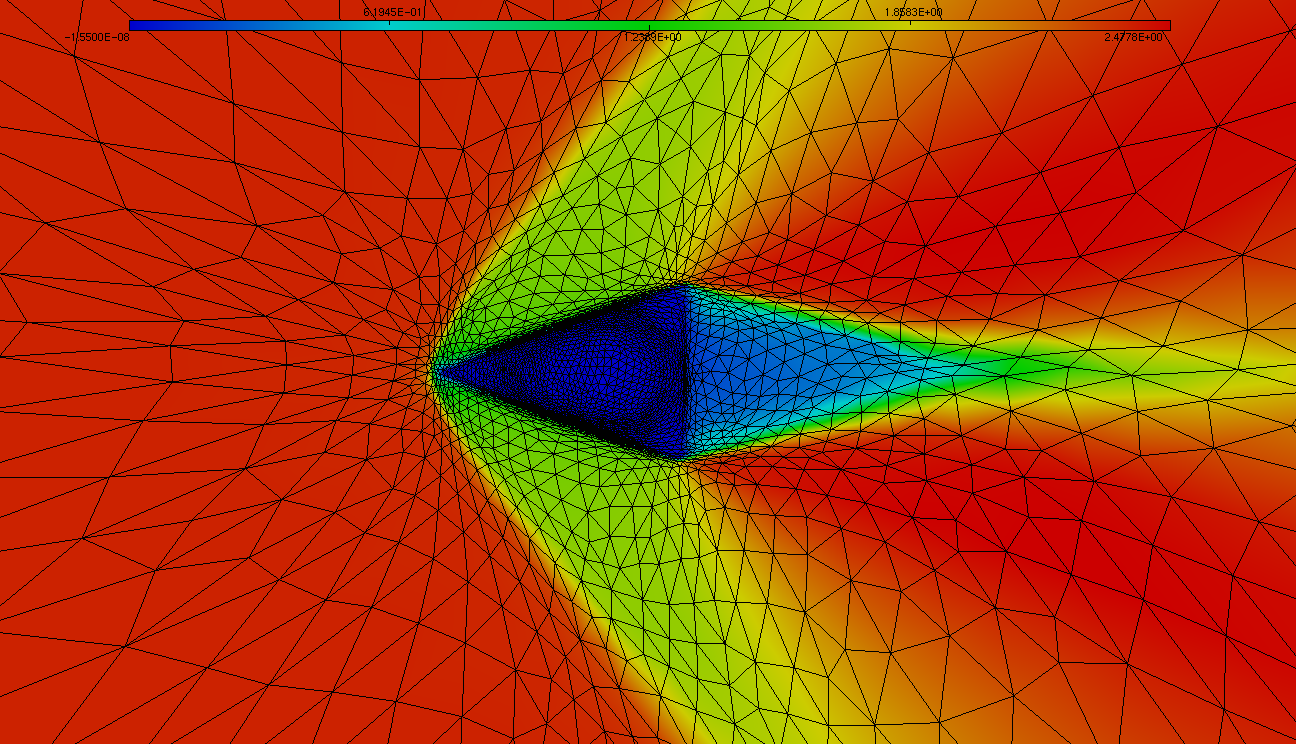
\includegraphics[scale=.15]{Bordeaux/figures/AdapPhysique/u.png}
		\captionof{subfigure}{Composant horizontale de la vitesse}
	\end{minipage}
	\hfill
	\begin{minipage}[t]{.5\linewidth}
		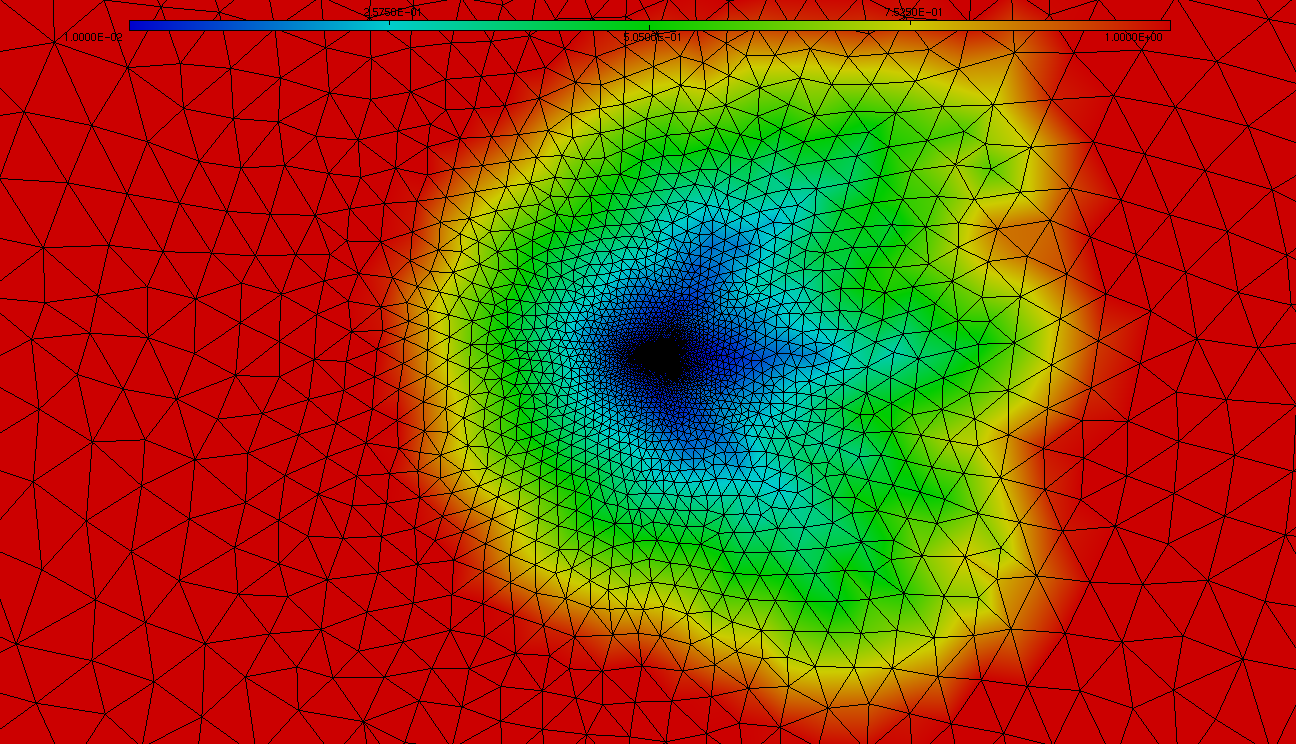
\includegraphics[scale=.15]{Bordeaux/figures/AdapPhysique/met.png}
		\captionof{subfigure}{Tailles calculées à partir de la métrique associée}
	\end{minipage}	
	\captionof{figure}{Écoulement autour d'un triangle - calcul des tailles désirées à partir d'une variable physique \label{fig:metPhys}}
\endgroup

\indent

\indent Aussi comme dans le cas de l'adaptation à des fonctions Level Set, on a plutôt utilisé dans l'adaptation physique le calcul des tailles désirées pour déterminer le mouvement des points du maillage. Les raisons sont les mêmes que celles présentées précédemment : du point de vue de l'utilisateur final, cette procédure, qui demande la définition des seuils pour la taille désirée, a un sens physique intuitif, étant ainsi plus accessible.

\subsection{Couplage entre adaptation Level Set et adaptation physique}

\indent L'objectif principal de l'ensemble du travail réalisée dans ce projet est l'application du modèle et de la bibliothèque développés à la résolution de problèmes de la mécanique de fluides, afin d'améliorer la précision des résultats. Ainsi, un bon maillage serait adapté au même temps à la surface de l'objet dans le domaine et au profil de la variable physique calculée (la vitesse, par exemple), et par conséquent les deux types de adaptation présentées ci-dessus doivent être considérées.

\indent Pour coupler les deux adaptations, on intersecte ses respectives métriques: en notant \(h_i^{LS}\) et \(h_i^{phys}\) la taille calculée pour le noeud \(i\) à partir des métriques, respectivement, de la fonction Level Set et de la variable physique (avant le lissage), on choisit le taille

\begin{equation*}
	h_i = \min(h_i^{LS},h_i^{phys})
\end{equation*}

\indent Ensuite, on applique le même lissage avec une gradation de 10\%.

\indent Pour le couplage des deux adaptations, on propose la procédure itérative suivante :  

\begin{enumerate}
	\item Calcul de la métrique associée à la fonction Level Set;
	\item Adaptation du maillage à cette métrique;
	\item \label{item:resolution} Résolution du problème physique sur le maillage adapté;
	\item Calcul de la métrique associée à la variable physique et intersection avec la métrique de la fonction Level Set;
	\item Adaptation du maillage à cette métrique, en partant du dernier maillage obtenu, mais toujours avec le même maillage de référence (le maillage de départ, non adapté);
	\item Retour au pas \ref{item:resolution}.
\end{enumerate}

\subsection{Résultats}

\indent La procédure décrite ci-dessus a été utilisé dans la résolution d'un flot supersonique 2D autour d'un triangle, avec une méthode de distribution de résidus appliquée aux équations de Navier Stokes pénalisées. Ce cas test est présenté et résolu dans \cite{leo}, dont les paramètres de l'écoulement sont les mêmes utilisés ici.

\indent Étant le modèle pénalisé, le triangle n'est pas discrétisée dans le domaine, ce qui signifie qu'il y a des mailles à son intérieur. En effet, le terme de pénalisation est appliqué exactement aux noeuds à l'intérieur de l'objet, identifiés par la signe de la fonction Level Set. Ainsi, la première adaptation de notre procédure (adaptation à la ligne de niveau 0 de la fonction Level Set) est de grande importance pour la représentation de la surface et la résolution précise des équations dans ses voisinages.

\indent La solution physique utilisée pour les adaptations suivantes est la composante horizontale de la vitesse. 

\indent Les tests ont été réalisées avec l'objectif de vérifier l'évolution de la qualité du résultat dans chaque itération de la procédure. Cette vérification a été faite de façon qualitative et quantitative. Pour la première, on a regardé par exemple la régularité du profil de la vitesse et de ses lignes de niveau et la résolution autour des coins du triangle. Pour la deuxième, on a adopté le même critère utilisé par \cite{leo}, en calculant l'angle entre le choc et l'axe \(y=0\), en utilisant un point du choc proche à cet axe, et identifiée par la proximité des lignes de niveau de la vitesse. La résolution analytique du problème fournit un angle \(\beta=53.33^o\), qu'on a utilisé pour la comparaison.

\indent Le résultat présenté dans les figures \ref{fig:adapPhysDoms} à \ref{fig:adapPhysPlotB} a été fait sur un domaine circulaire, de rayon vingt fois plus grand que la taille du triangle, afin de représenter un domaine infini, qui minimise l'influence des bords. Afin d'éviter un nombre trop grand de points, mais encore avec un bon raffinement dans les régions les plus proches des bords pour bien capturer le choc, les tailles des éléments ont été définies en fonction de la distance au centre du domaine, augmentant linéairement entre 0.002 et 1. Le résultat est un maillage avec 12664 noeuds et 25200 éléments.

\indent

\begingroup
	\begin{minipage}[t]{.5\linewidth}
		\centering
		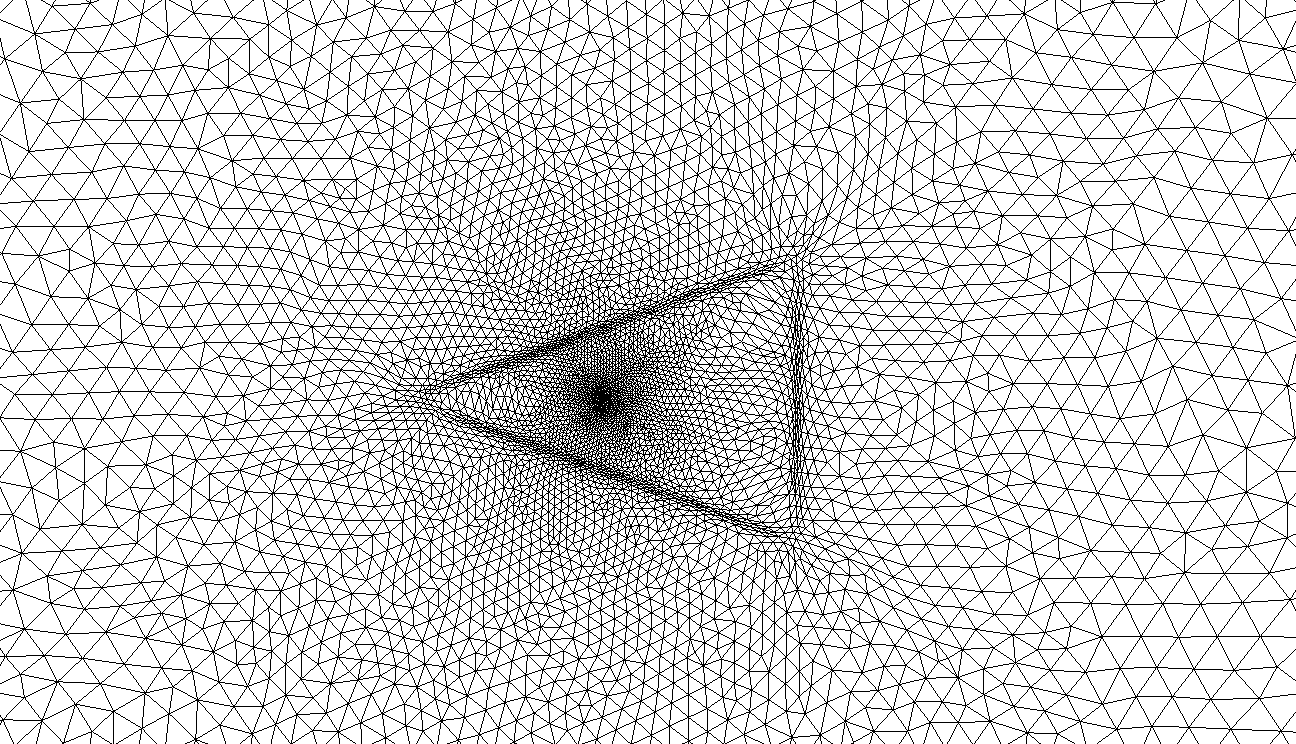
\includegraphics[scale=.15]{Bordeaux/figures/AdapPhysique/dom4bI0.png}
		\captionof{subfigure}{Première adaptation}
	\end{minipage}
	\hfill
	\begin{minipage}[t]{.5\linewidth}
		\centering
		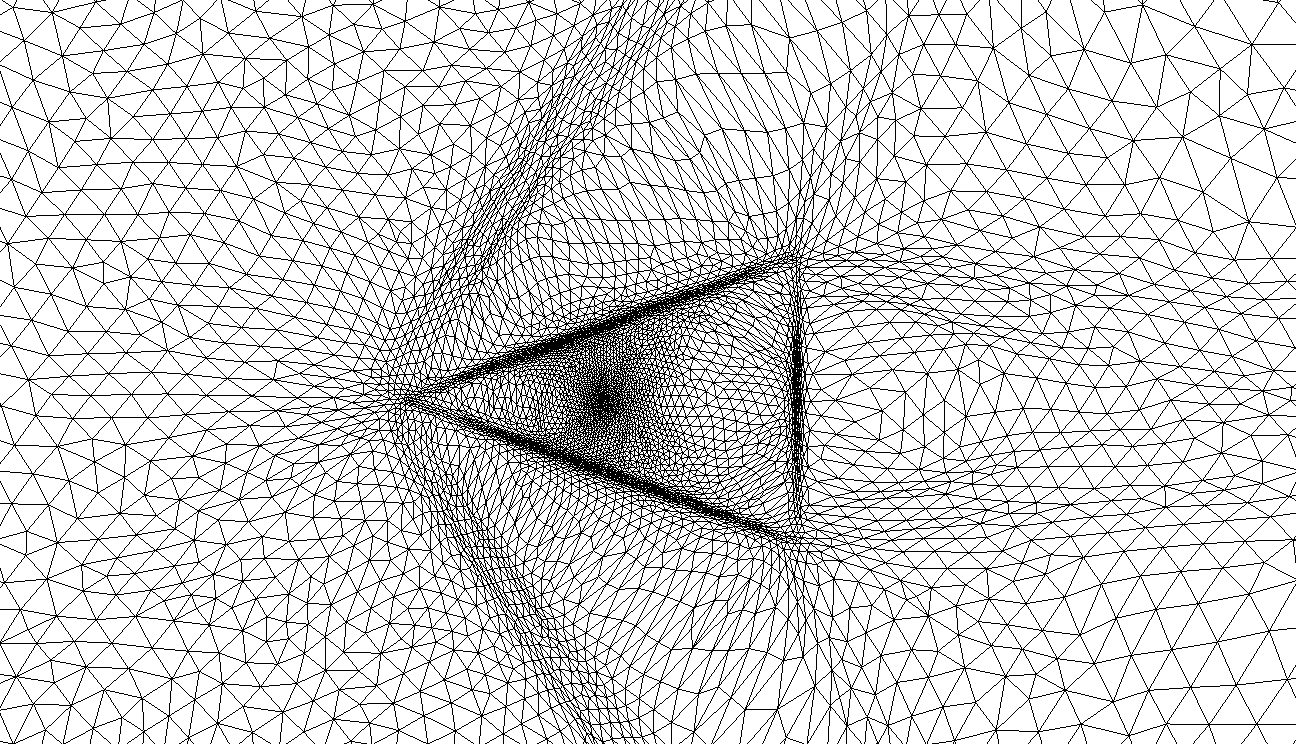
\includegraphics[scale=.15]{Bordeaux/figures/AdapPhysique/dom4bI1.png}
		\captionof{subfigure}{Deuxième adaptation}
	\end{minipage}
	\begin{minipage}[t]{1.\linewidth}
		\centering
		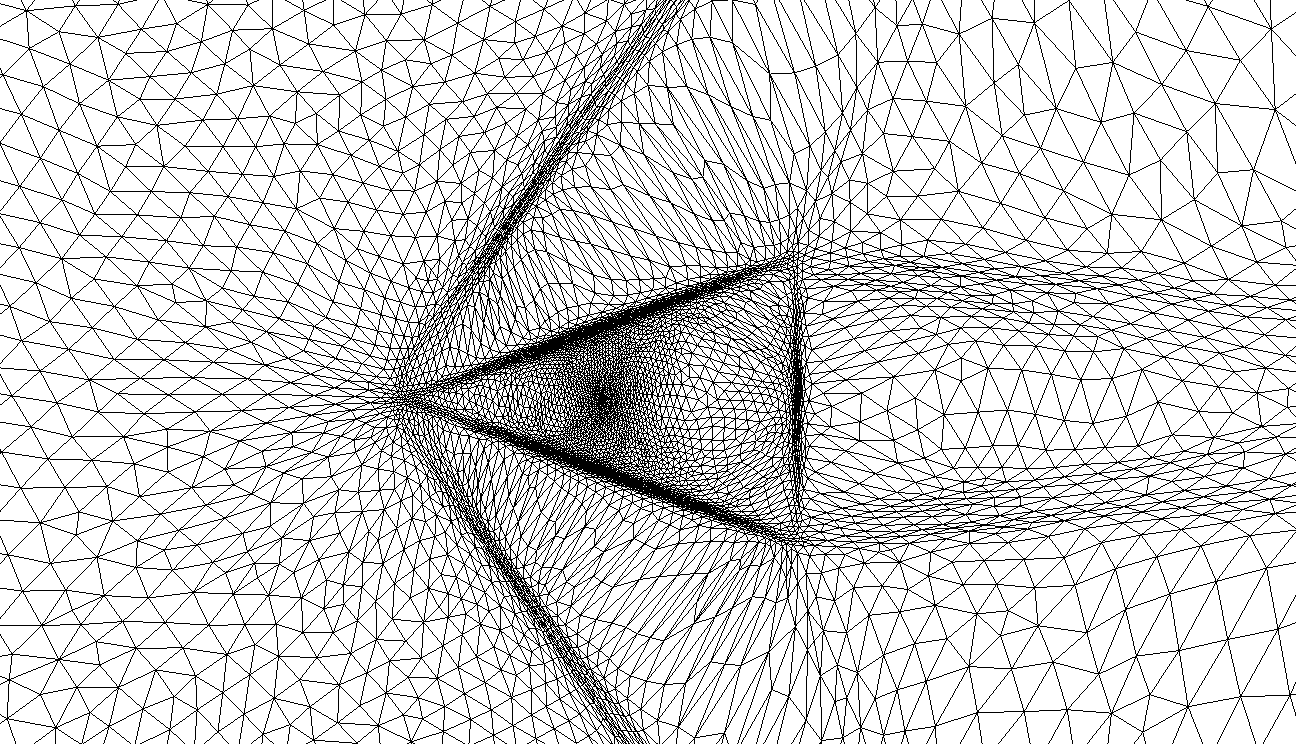
\includegraphics[scale=.15]{Bordeaux/figures/AdapPhysique/dom4bI2.png}
		\captionof{subfigure}{Troisième adaptation}
	\end{minipage}
	\captionof{figure}{Séquence de maillages adaptés obtenus \label{fig:adapPhysDoms}}
\endgroup

\newpage

\begingroup
	\begin{minipage}[t]{.5\linewidth}
		\centering
		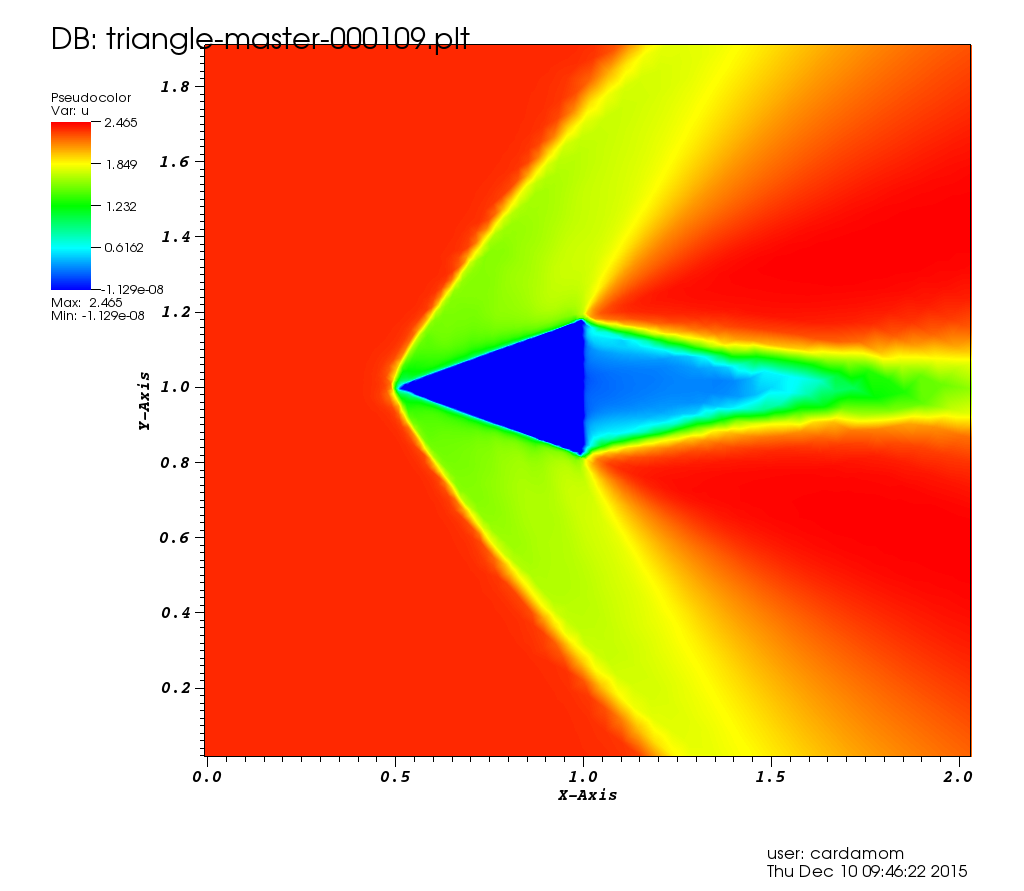
\includegraphics[scale=.2]{Bordeaux/figures/AdapPhysique/Plot4bI0A.png}
		\captionof{subfigure}{Première résolution}
	\end{minipage}
	\hfill
	\begin{minipage}[t]{.5\linewidth}
		\centering
		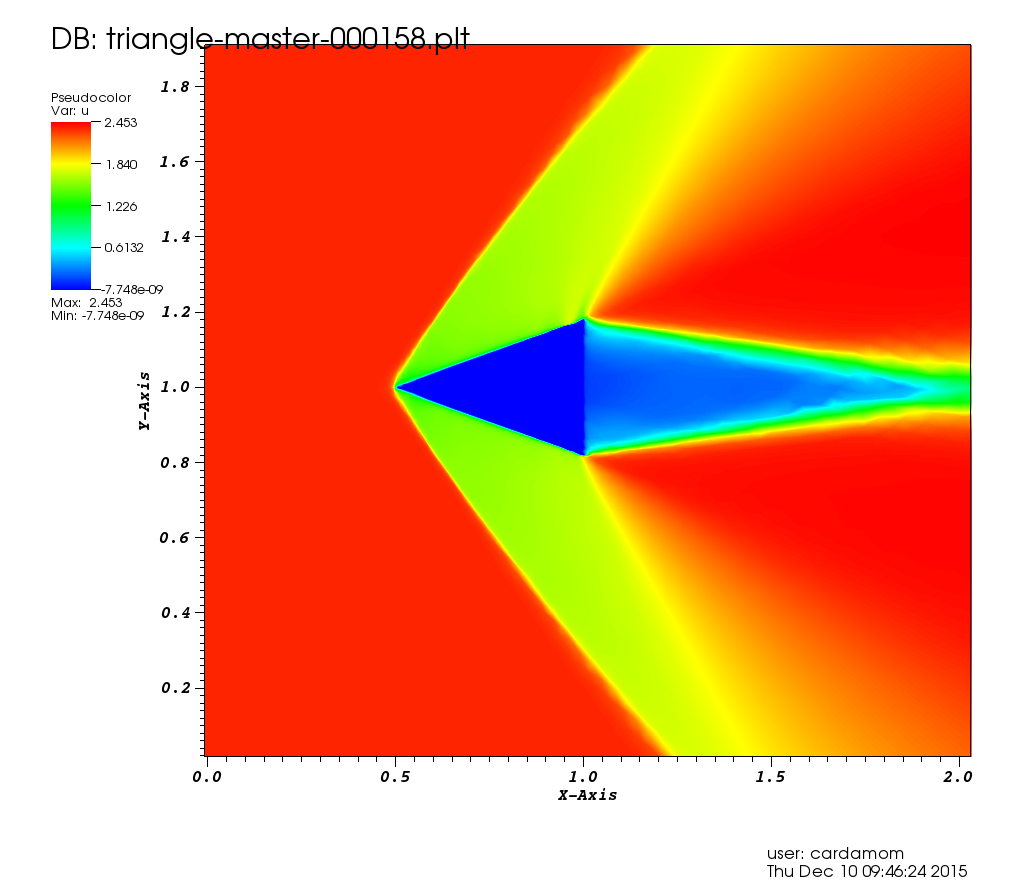
\includegraphics[scale=.2]{Bordeaux/figures/AdapPhysique/Plot4bI1A.png}
		\captionof{subfigure}{Deuxième résolution}
	\end{minipage}
	\begin{minipage}[t]{1.\linewidth}
		\centering
		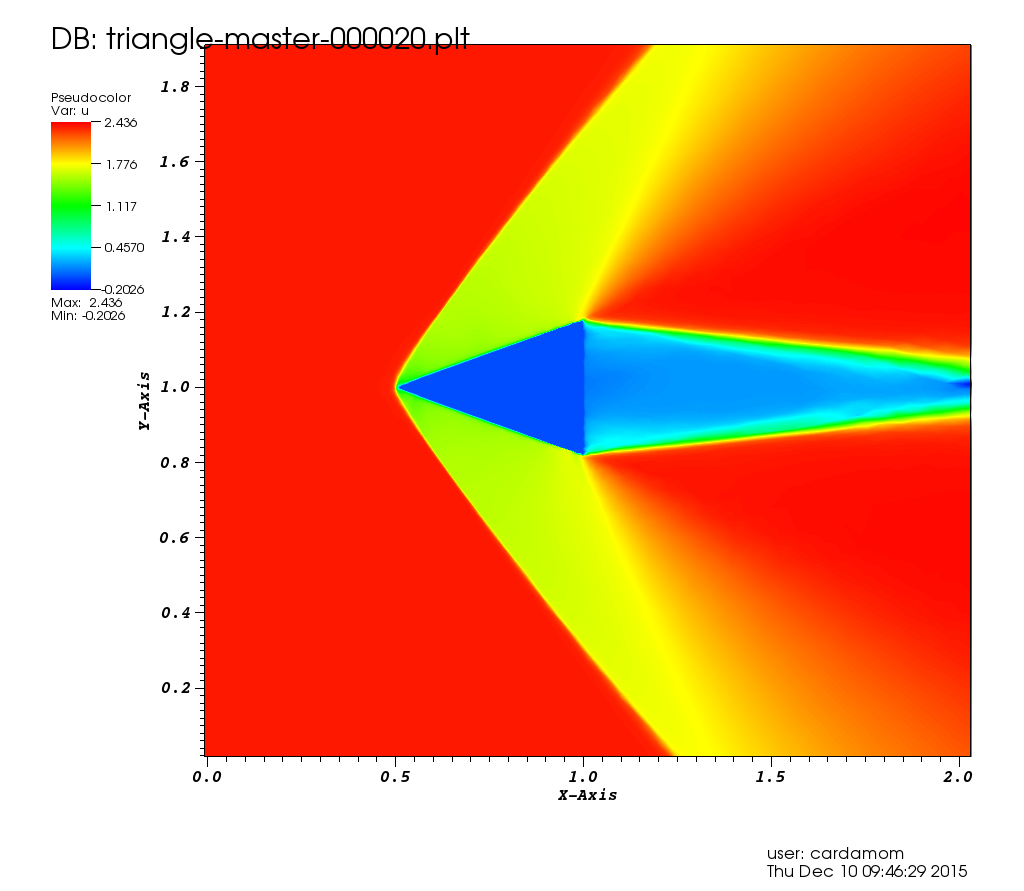
\includegraphics[scale=.2]{Bordeaux/figures/AdapPhysique/Plot4bI2A.png}
		\captionof{subfigure}{Troisième résolution}
	\end{minipage}
	\captionof{figure}{Composante horizontale de la vitesse \label{fig:adapPhysPlotA}}
\endgroup

\newpage

\begingroup
	\begin{minipage}[t]{.5\linewidth}
		\centering
		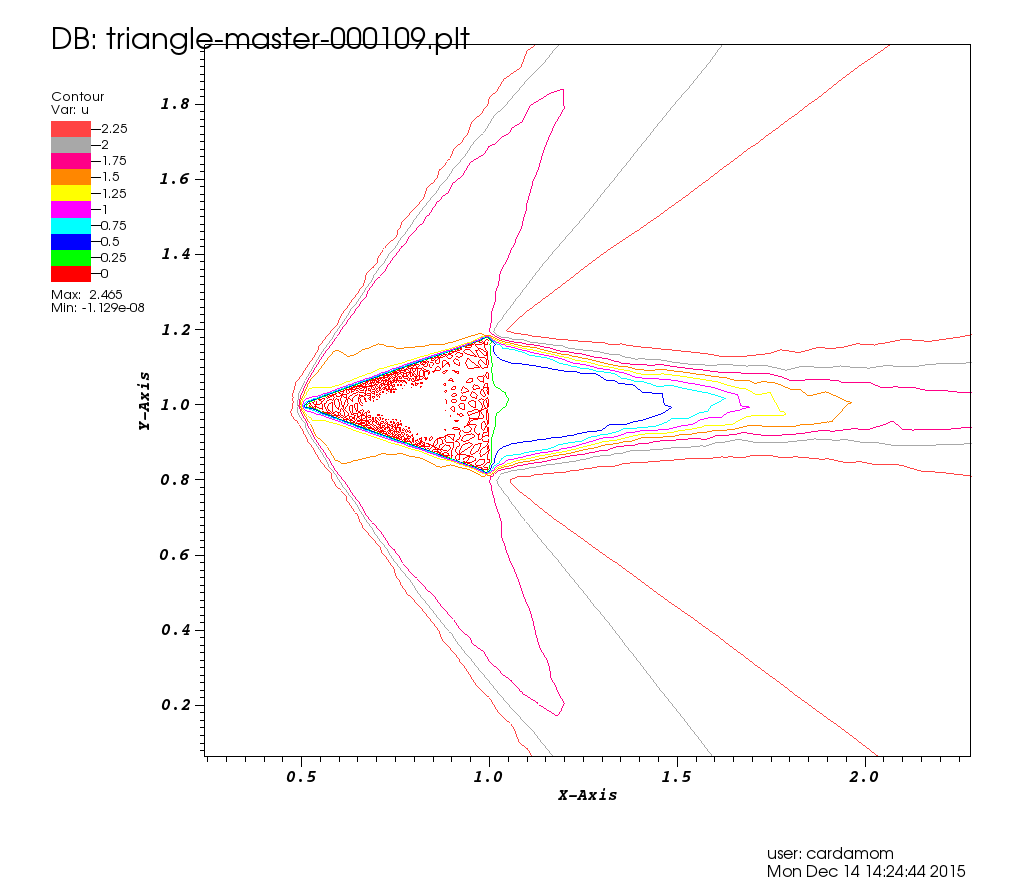
\includegraphics[scale=.2]{Bordeaux/figures/AdapPhysique/Contour4bI0.png}
		\captionof{subfigure}{Première résolution}
	\end{minipage}
	\hfill
	\begin{minipage}[t]{.5\linewidth}
		\centering
		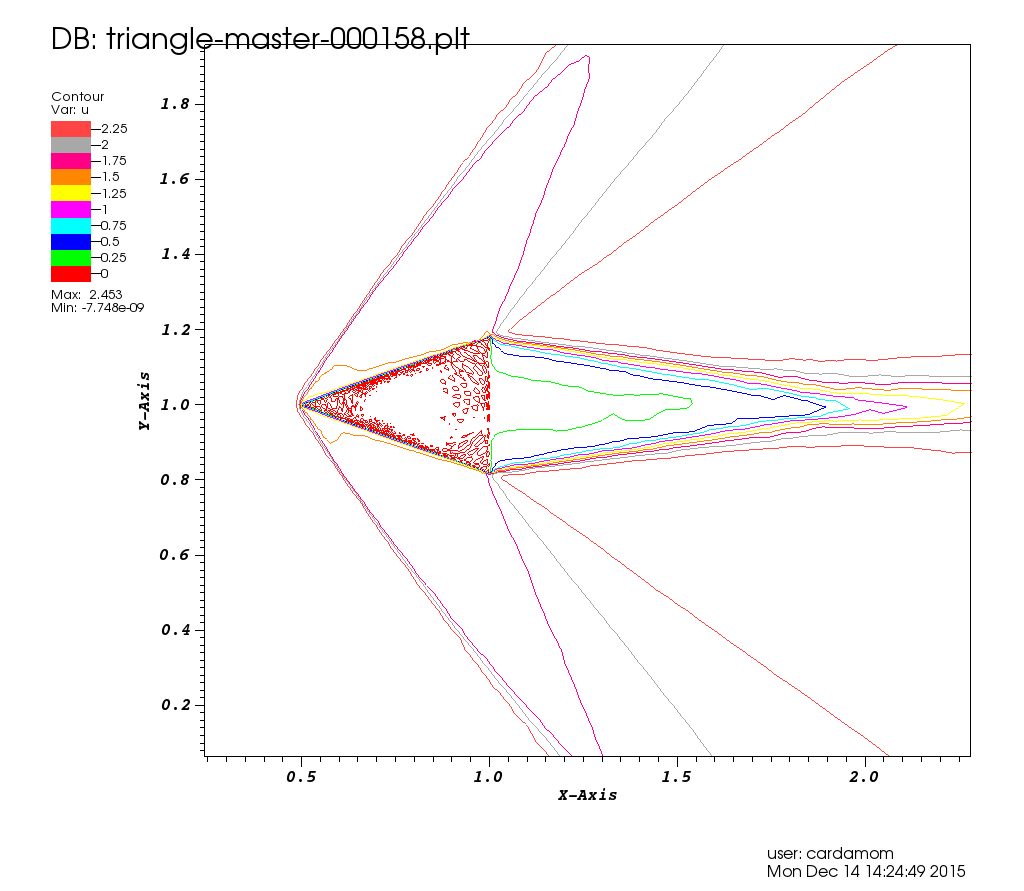
\includegraphics[scale=.2]{Bordeaux/figures/AdapPhysique/Contour4bI1.png}
		\captionof{subfigure}{Deuxième résolution}
	\end{minipage}
	\begin{minipage}[t]{1.\linewidth}
		\centering
		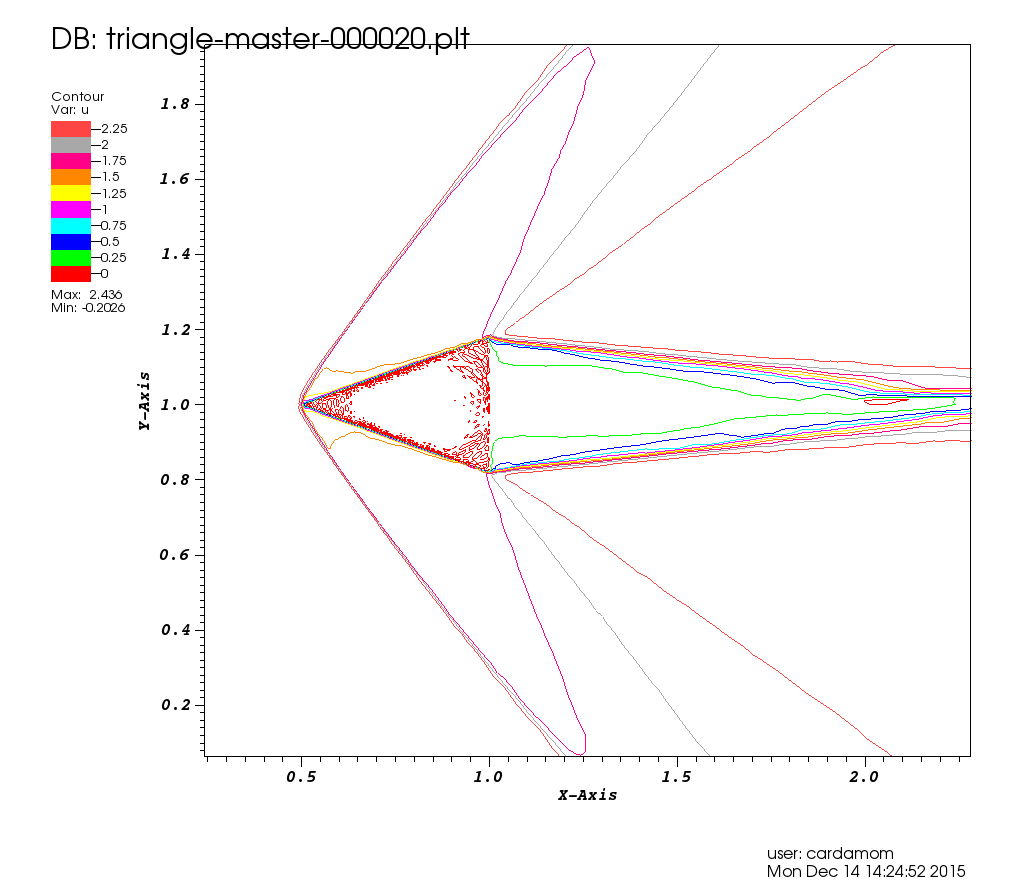
\includegraphics[scale=.2]{Bordeaux/figures/AdapPhysique/Contour4bI2.png}
		\captionof{subfigure}{Troisième résolution}
	\end{minipage}
	\captionof{figure}{Lignes de niveau de la composante horizontale de la vitesse \label{fig:adapPhysContour}}
\endgroup

\newpage

\begingroup
	\begin{minipage}[t]{.5\linewidth}
		\centering
		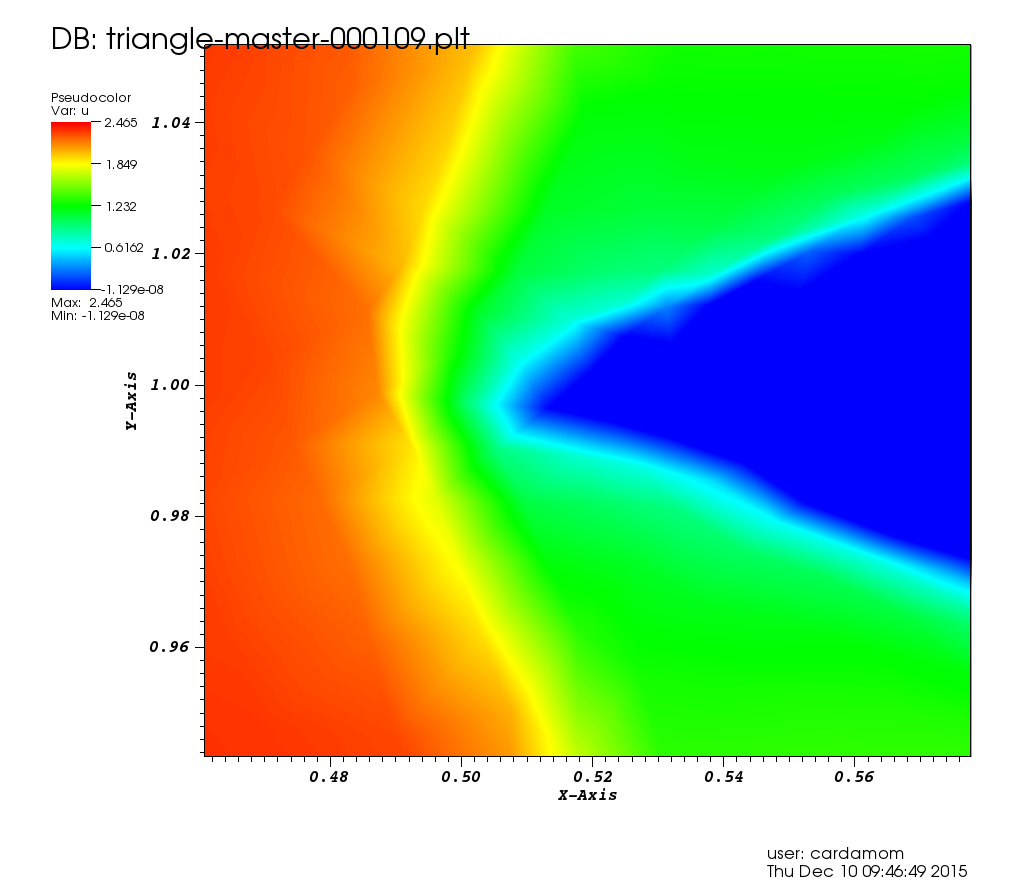
\includegraphics[scale=.2]{Bordeaux/figures/AdapPhysique/Plot4bI0B.png}
		\captionof{subfigure}{Première résolution}
	\end{minipage}
	\begin{minipage}[t]{.5\linewidth}
		\centering
		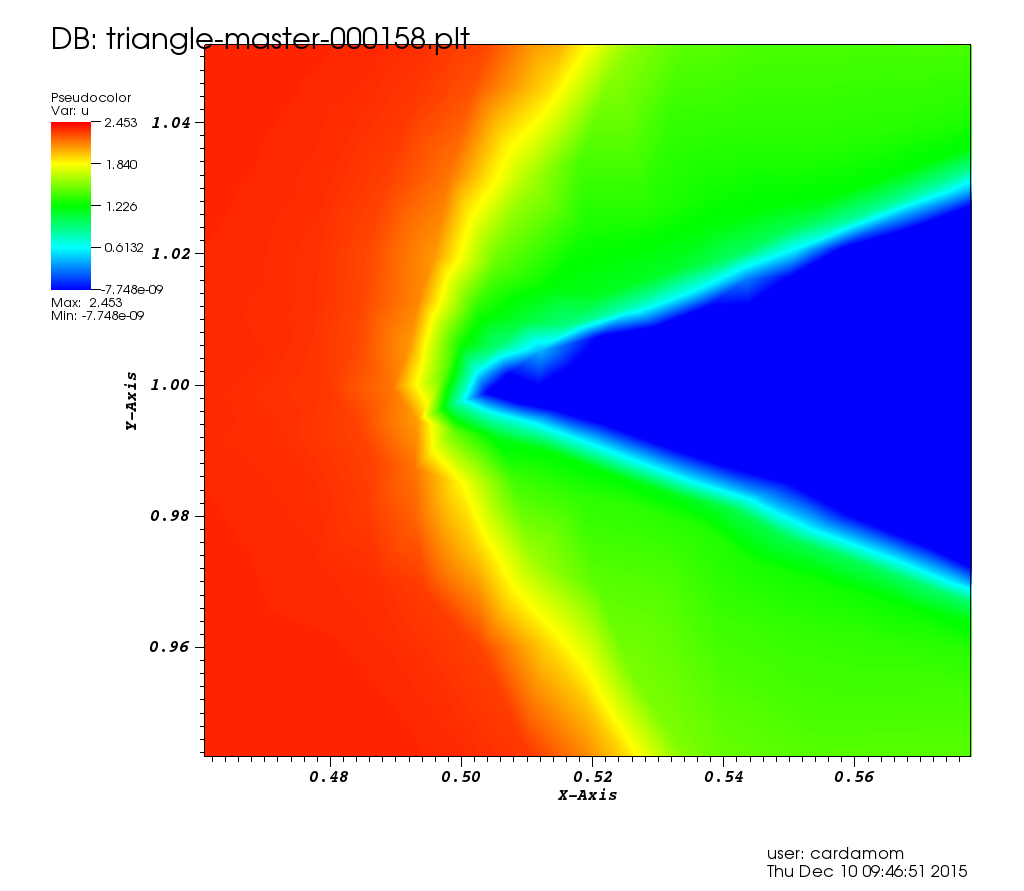
\includegraphics[scale=.2]{Bordeaux/figures/AdapPhysique/Plot4bI1B.png}
		\captionof{subfigure}{Deuxième résolution}
	\end{minipage}
	\begin{minipage}[t]{1.\linewidth}
		\centering
		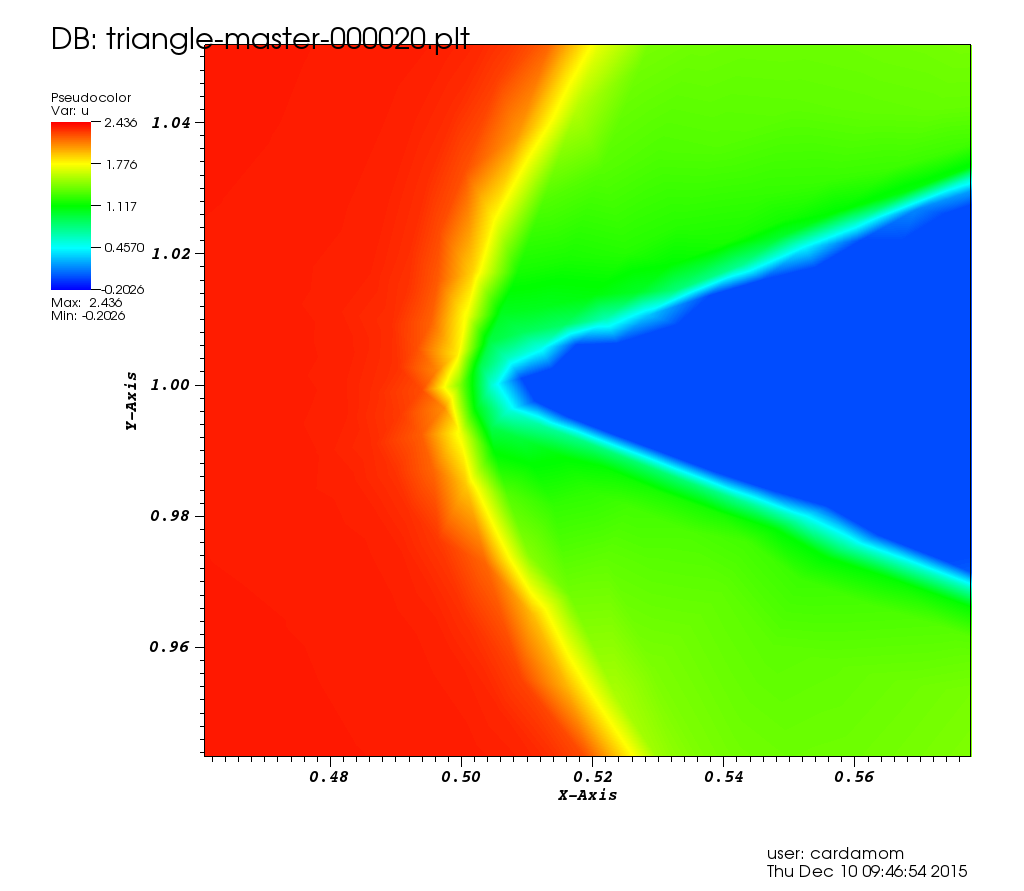
\includegraphics[scale=.2]{Bordeaux/figures/AdapPhysique/Plot4bI2B.png}
		\captionof{subfigure}{Troisième résolution}
	\end{minipage}
	\captionof{figure}{Détail - Composante horizontale de la vitesse \label{fig:adapPhysPlotB}}
\endgroup

\indent

\indent L'angle \(\beta\) a évolué selon les valeurs présentées dans le tableau \ref{tab:beta}

\begin{table}[!ht]
	\centering
	\begin{tabular}{c|c}
		Résolution & \(\beta\) \\
		\hline
		1 & \(55.68^\circ\) \\
		2 & \(53.92^\circ\) \\
		3 & \(53.01^\circ\) \\
	\end{tabular}
	\caption{Angle entre le choc et l'axe \(y=0\) \label{tab:beta}}
\end{table}

\indent Ces résultats montrent que la procédure proposée permet en effet d'améliorer la résolution du problème physique : à chaque itération, le champ de vitesse calculée devient mieux définie, avec des lignes de niveau plus régulières, et l'angle entre le choc et l'axe \(y=0\) s'approche de la valeur analytique. Néanmoins, quelques difficultés sont encore présentes dans las tests réalisées, notamment la génération de maillages permettant un calcul stable (considérant les fortes discontinuités qui caractérisent ce cas test) et le fait que, comme montre la figure \ref{fig:adapPhysPlotB}, le choc n'est pas attaché au triangle, au contraire du résultat théorique, ce qui s'explique par les limitations du raffinement du maillage.
 
\section{Adaptation à un cas non stationnaire}
\label{sec:nonstat}

\indent Les résultats présentés dans les sections précédentes se référent à des cas stationnaires, avec les surfaces fixes, mais une situation qu'on veut considérer aussi  est celle où les objets bougent. Dans ce cas, il faut à chaque pas de temps actualiser la fonction Level Set et adapter le maillage autour de la nouvelle position de la surface. La procédure adoptée est la suivante : 

\begin{enumerate}
	\item Pour tout noeud du maillage, calculer la fonction Level Set par rapport à la position actuelle de l'objet, et la fonction \(u\) à adapter (equation \eqref{eq:atan});
	\item Adapter le maillage à la fonction \(u\);
	\item Faire bouger la surface de l'objet (indépendamment de la position des noeuds)
\end{enumerate}

\indent L'objectif de cette procédure est de faire chaque adaptation à partir du dernier maillage adapté, au lieu de partir du maillage non adapté à chaque pas du mouvement. Ainsi, on peut éviter de garder en mémoire toute la structure du maillage de référence et du maillage adapté. Il faut pourtant garder au moins les aires et les vecteurs normaux du maillage, parce que, en raison du modèle adopté, toutes les adaptations doivent utiliser le même maillage de référence.

\indent Les figures \ref{fig:circleLSAdv} et \ref{fig:nacaLSAdv} présentent deux exemples de cette procédure, le premier pour l'advection d'un cercle et le deuxième pour l'oscillation de l'aile Naca. Les mouvements on été discrétisées en 20 pas de temps, et chaque itération a été réalisée avec 20 ou 30 itérations, respectivement.

\indent On peut observer qu'on obtient à chaque pas de temps une bonne adaptation à la position actuelle de la fonction Level Set, mais que les positions précédentes ne sont pas complètement ``désadaptées", même que son trace soit faible. En effet, les tests montrent que le passage d'une adaptation à la prochaine se fait de deux manières (en dépendant de la position des points adaptés pour la position précédente) : soit par le mouvement des points d'une région adaptée à l'autre (ce qui est possible quand le point est relativement proche de la nouvelle position de l'objet), soit par le ``dérafinement" d'une région (ce qui est le cas des points en amont du mouvement de l'objet). On a observé que le deuxième cas est plus lente que le premier, et ainsi on aurait besoin d'un plus grand nombre d'itérations. Néanmoins, pour justifier l'application de cette procédure, il faut trouver un équilibre entre le temps d'exécution et la qualité des résultats.

\indent

\begingroup
	\begin{minipage}[t]{.5\linewidth}
		\centering
		 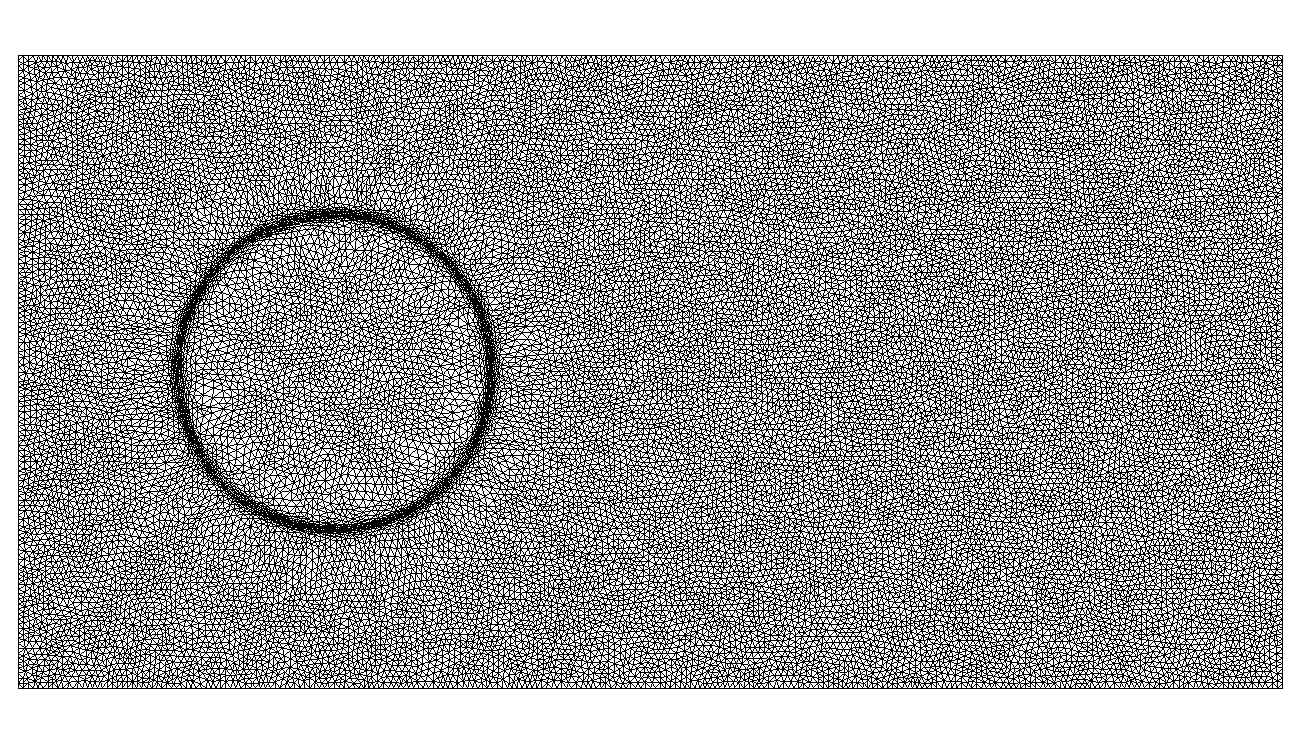
\includegraphics[scale=.15]{Bordeaux/figures/LSAdvection/CircleAdvNew0.png}
		 \captionof{subfigure}{Pas n. 0}
	\end{minipage}
	\begin{minipage}[t]{.5\linewidth}
		\centering
		 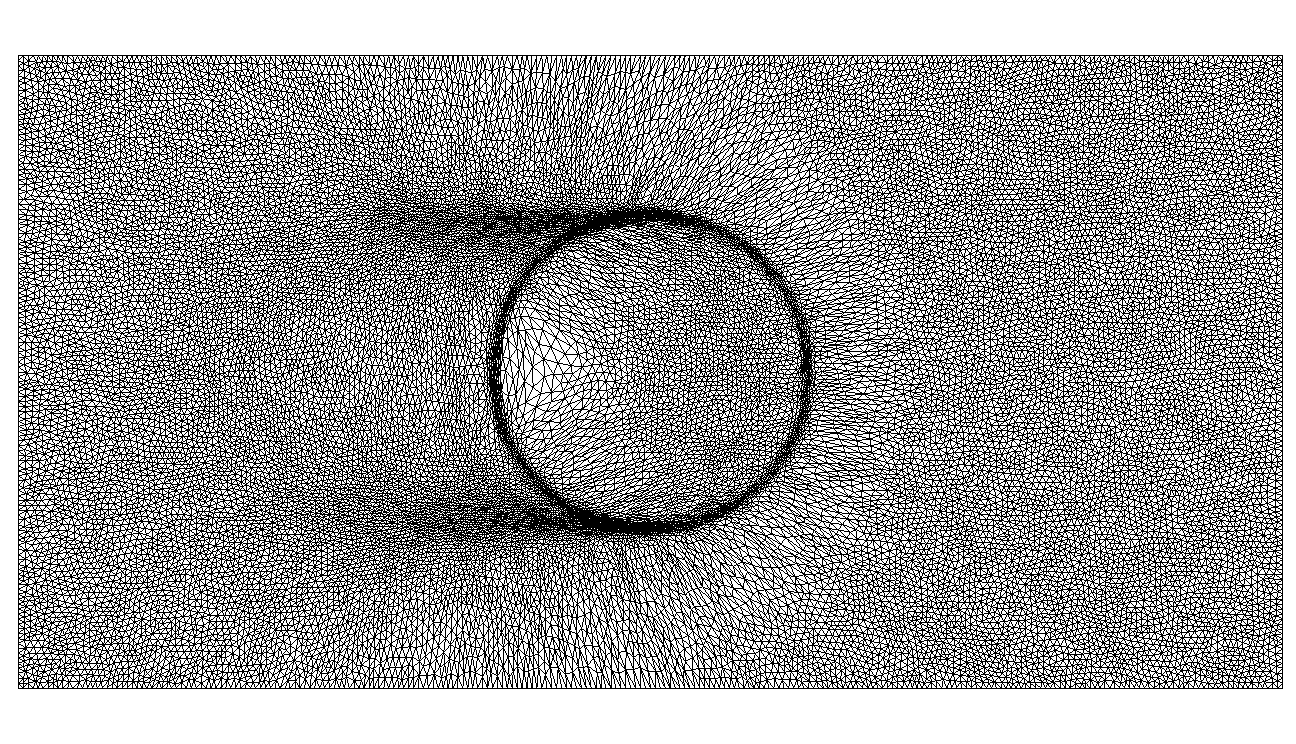
\includegraphics[scale=.15]{Bordeaux/figures/LSAdvection/CircleAdvNew10.png}
		 \captionof{subfigure}{Pas n. 10}
	\end{minipage}
	\begin{minipage}[t]{1.\linewidth}
		\centering
		 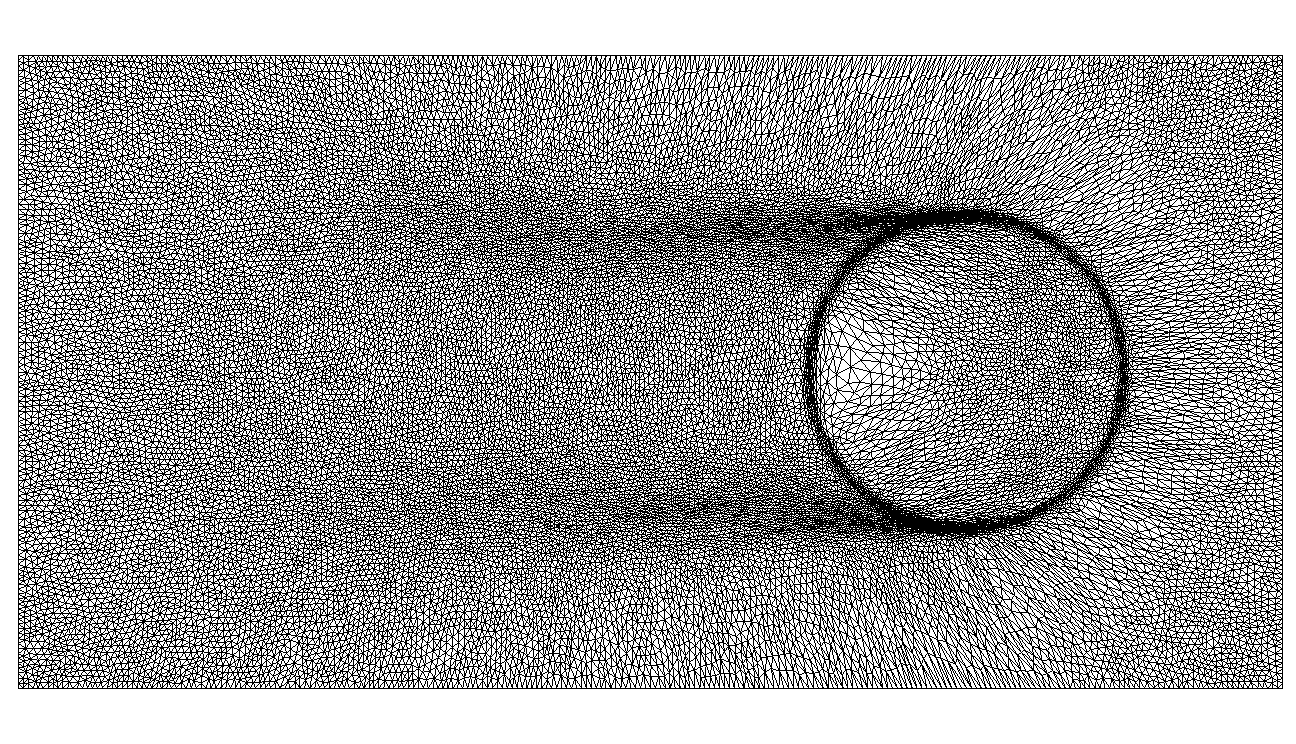
\includegraphics[scale=.15]{Bordeaux/figures/LSAdvection/CircleAdvNew20.png}
		 \captionof{subfigure}{Pas n. 20}
	\end{minipage}
	\captionof{figure}{Advection d'un cercle \label{fig:circleLSAdv}}
\endgroup

\indent

\indent

\begingroup
	\begin{minipage}[t]{.5\linewidth}
		\centering
		 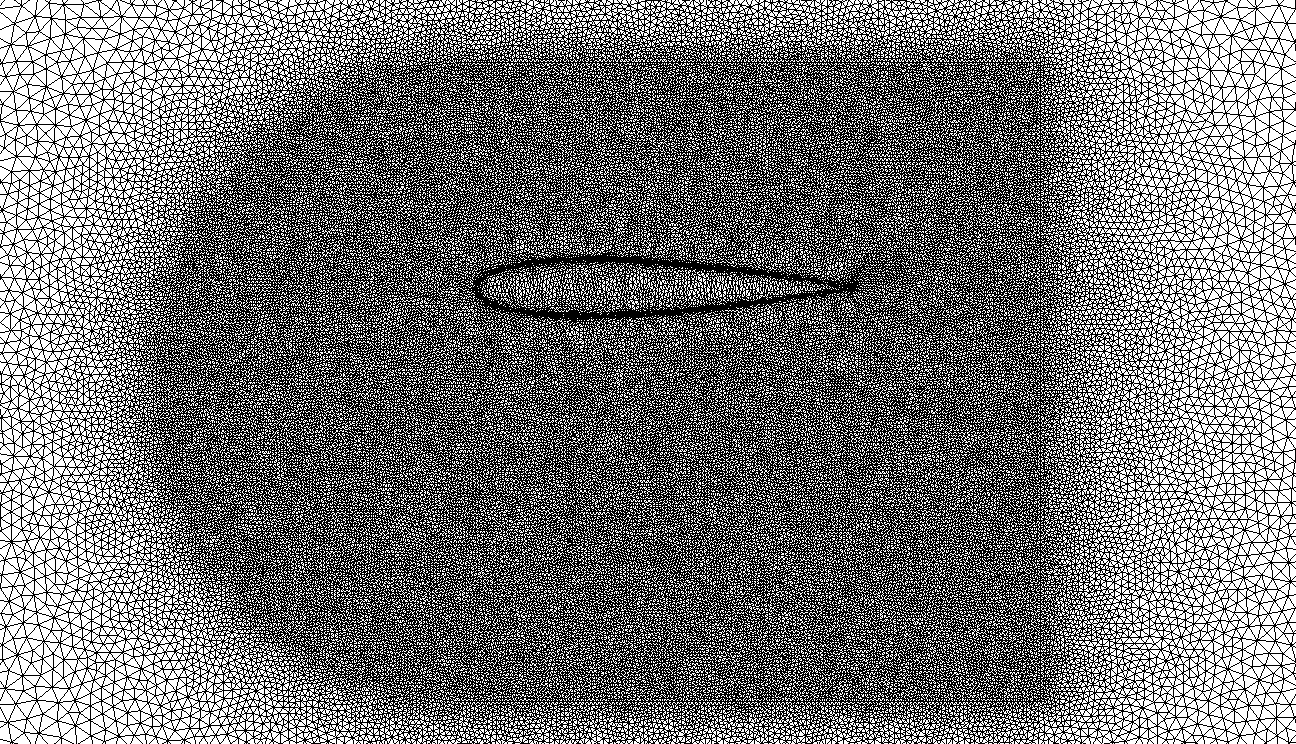
\includegraphics[scale=.15]{Bordeaux/figures/LSAdvection/NacaAdvNew0.png}
		 \captionof{subfigure}{Pas n. 0}
	\end{minipage}
	\begin{minipage}[t]{.5\linewidth}
		\centering
		 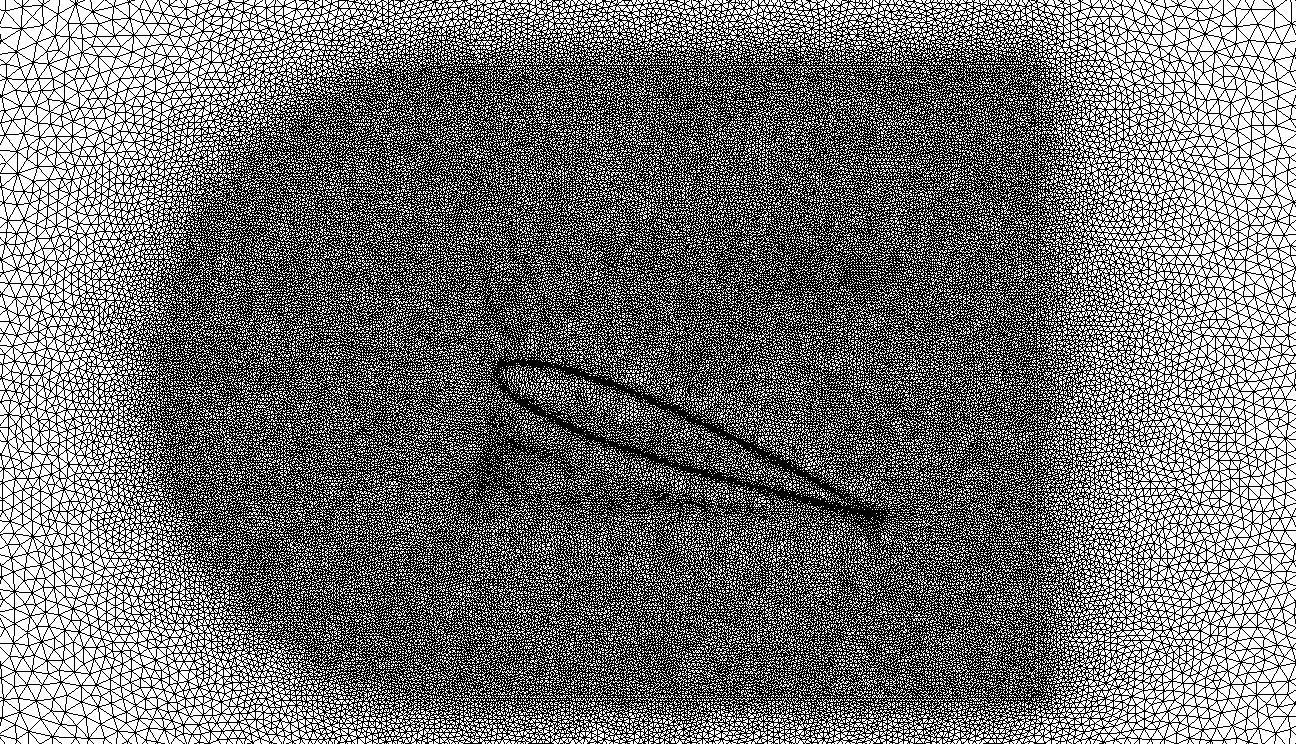
\includegraphics[scale=.15]{Bordeaux/figures/LSAdvection/NacaAdvNew10.png}
		 \captionof{subfigure}{Pas n. 10}
	\end{minipage}
	\begin{minipage}[t]{1.\linewidth}
		\centering
		 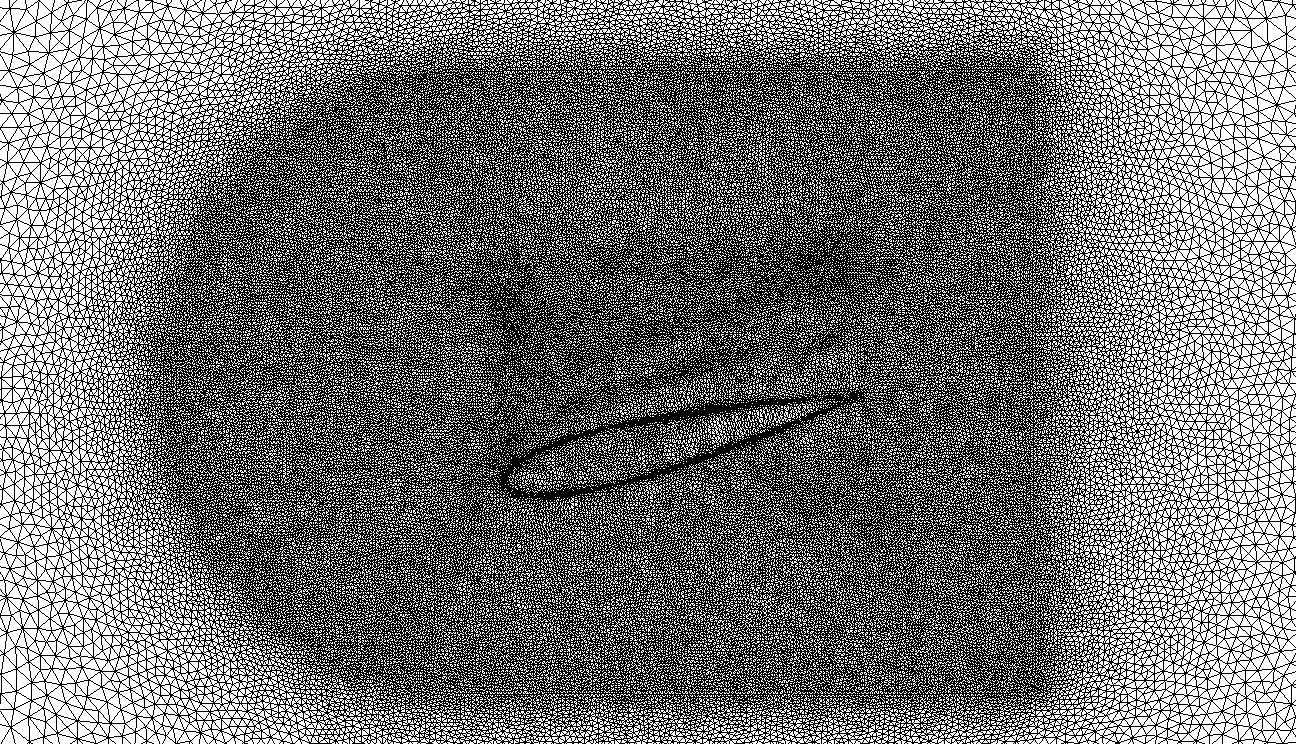
\includegraphics[scale=.15]{Bordeaux/figures/LSAdvection/NacaAdvNew20.png}
		 \captionof{subfigure}{Pas n. 20}
	\end{minipage}
	\captionof{figure}{Naca oscillant \label{fig:nacaLSAdv}}
\endgroup



%\indent L'approche qu'on a d'abord essayé, envisageant une économie de l'espace mémoire utilisé pour l'exécution du programme, était de faire l'adaptation, à chaque pas de temps, à partir du dernier maillage calculé. Néanmoins, les tests ont présenté plusieurs problèmes qui se montrent incontournables avec le modèle d'adaptation qu'on utilise, notamment : 
%
%\begin{itemize}
%	\item Le modèle ne provoque pas un "dé-raffinement" des éléments. Ainsi, dans le résultat final, on peut observer le trace de la marche de l'objet sur le maillage (figure \ref{fig:optim_bad});
%	\item Les éléments raffinés dans un certain pas de temps n'arrivent pas à bouger jusqu'à la nouvelle position, soit en raison de la très fréquente relaxation (principalement quand on discrétise le mouvement de la surface avec un petit pas de temps, car les adaptations successives sont faites presque sur le même endroit), soit parce qu'il sont très éloignés de la nouvelle position (principalement quand le pas de temps est trop grand).
%\end{itemize}
%
%	\begin{figure} [!ht]
%	  \begin{subfigure}{.5\linewidth}
%	    \centering
%	    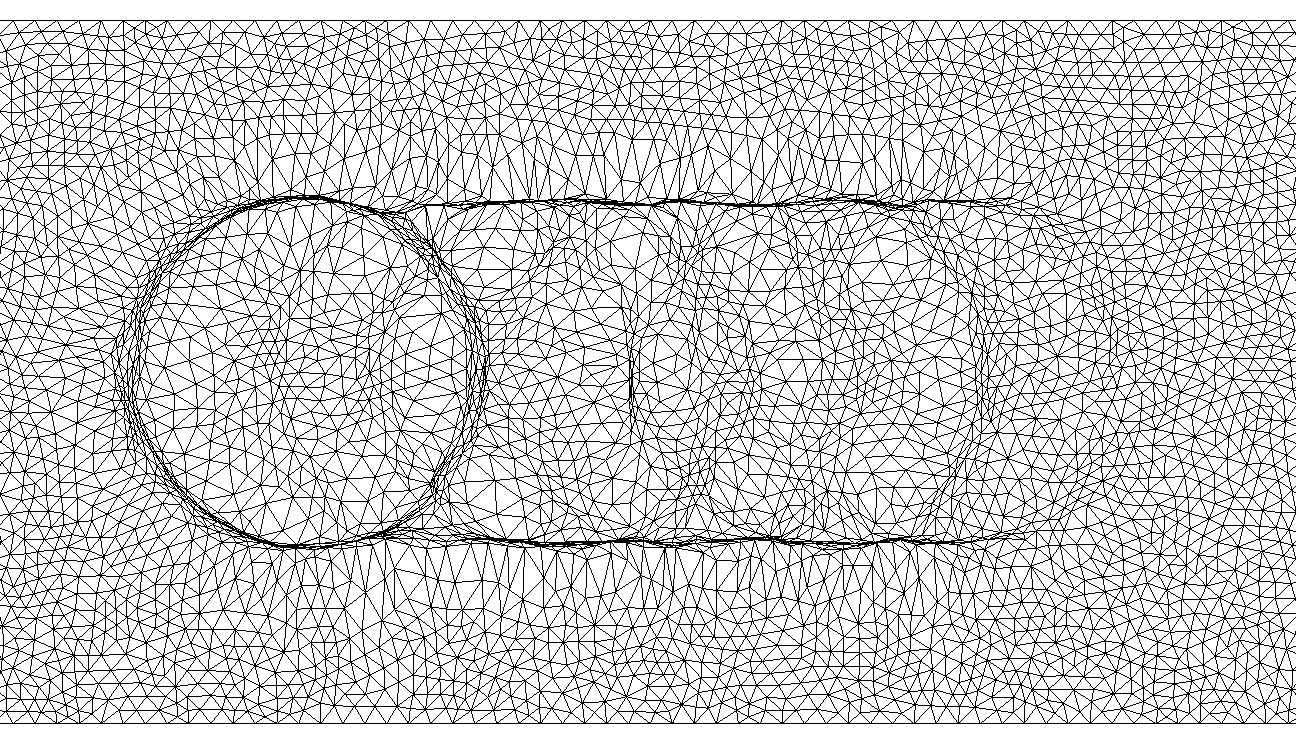
\includegraphics[scale=.12]{figures/optim_bad_circle.png}
%	  \end{subfigure} 
%	  \begin{subfigure}{.5\linewidth}
%	    \centering
%	    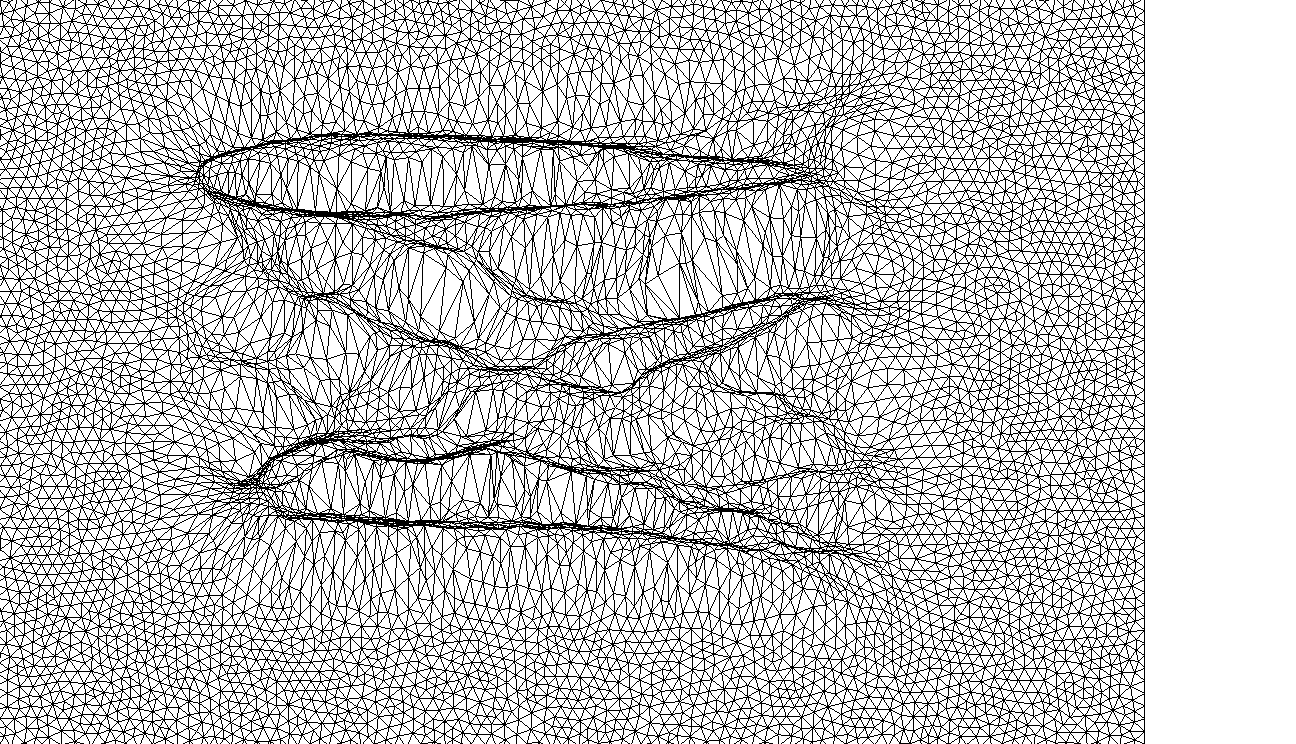
\includegraphics[scale=.12]{figures/optim_bad_naca.png}
%	  \end{subfigure}
%	  \caption{Maillages finaux des adaptions partant du maillage initial à chaque pas du mouvement de la surface \label{fig:optim_bad}}
%	\end{figure}
%
%\indent L'unique solution trouvée, ainsi, est de faire chaque adaptation en partant toujours du maillage initial. On obtient ainsi des très bons résultats, comme montrent les figures \ref{fig:optim_good_1} et \ref{fig:optim_good_2}, car les adaptations sont indépendantes, mais pour cela il faut garder le maillage initial en mémoire.
%
%	\begin{figure} [!ht]
%	  \begin{subfigure}{.5\linewidth}
%	    \centering
%	    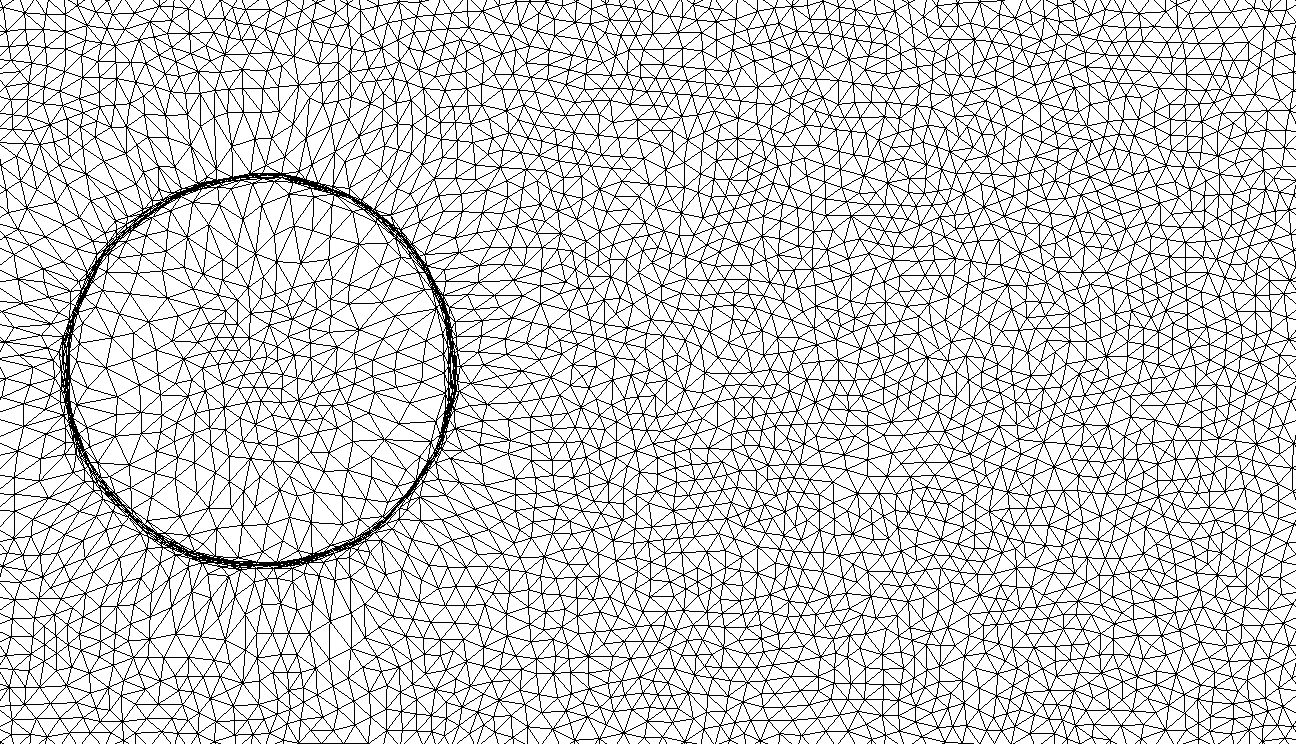
\includegraphics[scale=.12]{figures/optim_good_circle0.png}
%	  \end{subfigure} 
%	  \begin{subfigure}{.5\linewidth}
%	    \centering
%	    \includegraphics[scale=.12]{figures/optim_good_circle1.png}
%	  \end{subfigure}
%	  \begin{subfigure}{.5\linewidth}
%	    \centering
%	    \includegraphics[scale=.12]{figures/optim_good_circle2.png}
%	  \end{subfigure}
%	  \begin{subfigure}{.5\linewidth}
%	    \centering
%	    \includegraphics[scale=.12]{figures/optim_good_circle3.png}
%	  \end{subfigure} 
%	  \caption{Adaptation à un cercle advecté \label{fig:optim_good_1}}
%	\end{figure}
%	
%	\begin{figure} [!ht]
%	  \begin{subfigure}{.5\linewidth}
%	    \centering
%	    \includegraphics[scale=.12]{figures/optim_good_naca0.png}
%	  \end{subfigure} 
%	  \begin{subfigure}{.5\linewidth}
%	    \centering
%	    \includegraphics[scale=.12]{figures/optim_good_naca1.png}
%	  \end{subfigure}
%	  \caption{Adaptation au Naca oscillant \label{fig:optim_good_2}}
%	\end{figure}


\part{Meric / Inria Chile - Méthodes de Décomposition de Domaine}
\section{Introduction}

\indent Le travail réalisée dans le deuxième stage de mon année de césure s'insère dans le contexte et les objectives de Meric : la recherche scientifique multidisciplinaire liée à la production d'énergie Marine au Chili. Plus spécifiquement, je faisait partie de l'équipe responsable pour la ligne d'investigation appelé ``Modélisation avancée pour l'énergie marine'', dont le principal objectif sont le ``couplage de modèles de petites résolutions spectrales a des grandes résolutions dans le domaine du espace-temps'' et ``la modélisation de grande résolution spatiale et temporale proche de la côte''\footnote{http://www.meric.cl/que-hacemos/}.

\indent Les sujets étudiés dans ce stage constituent une introduction à la recherche envisageant ces objectifs et peuvent être divisés en deux branches principales: la première consiste dans l'étude, implémentation numérique et simulation de modèles de propagation d'ondes d'eau; le deuxième, plus directement lié à la ligne de recherche de Meric, envisage l'étude, développement et application numérique de méthodes de décomposition de domaine (DDMs) pour la résolution de tels modèles.

\indent Concernant le premier point, on a étudié plusieurs modèles qui prennent en compte les effets non linéaires et dispersives dans la propagation des ondes. Cet étude s'est focalisé notamment sur l'équation de KdV et l'équation de Serre. En considérant les objectifs de la recherche développé par l'équipe, l'étude de différentes modèles mathématiques a une grande importance : premièrement, chacun d'eux est dérivée à partir d'hypothèses différents, et, ainsi, ses domaines de validité physique sont différents. Des critères comme les caractéristiques de l'onde (amplitude et longueur), la profondeur de l'eau et le fond océanique guident le choix d'un ou autre modèle. Dans le contexte de la production de l'énergie marine, par exemple, la distance à la côte est très importante, et le choix du bon modèle est essentielle pour que les variables d'intérêt, comme la vitesse et l'amplitude des ondes, peuvent être calculées de manière fiable.

\indent Par ailleurs, en raison des différentes complexités de chaque modèle, les approches nécessaires pour son étude dans le contexte des méthodes de décomposition de domaine sont aussi différents. Dans ce stage, cet étude concernant l'équation de KdV a été bien avancé (entraînent même l'élaboration du papier scientifique qu'on a envoyé pour son publication); dans les dernières semaines du stage on a débuté l'étude de la résolution des équations de Serre avec des DDMs, mais encore sans des résultats pour présenter dans ce rapport.

\indent Les DDMs consistent en diviser un domaine cumputationnel en plusieurs subdomaines et résoudre un problème en chacun d'eux. Pour que la solution du problème décomposé soit la même que la solution du problème calculé dans le monodomaine, il est essentiel qu'on défini des conditions appropriés sur l'interface entre les subdomaines.

\indent Ainsi, dans la deuxième ligne de notre travail, on a d'abord fait un étude des conditions aux limites transparentes (TBCs) pour l'équation de KdV, en tenant compte que ces types de conditions aux bords jouent un rôle essentiel dans les méthodes de décomposition de domaine. Afin d'introduire ce sujet, on a suivi au début un approche plus simple, en optimisant des conditions aux bords classiques que fournissaient des conditions les plus proches des TBCs pour l'équation de KdV.

\indent Après, on s'est concentré dans l'étude des TBCs exactes pour l'équation de KdV linéarisée, en se basant sur l'es études développés par \cite{zheng2008} et \cite{besse2015}. Étant non locaux en temps, ces TBCs exactes ne peuvent pas être implémentées en pratique; alors notre but était de les proposer des approximation simples, qu'on a ensuite appliqué à une méthode de décomposition de domaine.

\indent À ce moment, il est nécessaire de clarifier et délimiter nos objectifs et les différences par rapport aux objectifs de \cite{zheng2008} et \cite{besse2015}. Pour cela, on fait une brève description des sources d'erreur et incertitudes liées aux simulations numériques de modèles physiques.

\indent De façon générale, ces erreurs peuvent être classifiés en des erreurs de modélisation conceptuelle et des erreurs numériques \cite{roache1997}. Dans le premier groupe, il y a les assomptions de modélisation conceptuelle (pour le phénomène physique et les conditions aux bords) et les incertitudes dans la géométrie, les donnés initiales, les donnés aux bords et les paramètres qui jouent un rôle dans le modèle \cite{roache1997,balagurusamy2008}. Dans ce qui concerne les erreurs numériques, on peut citer ceux liés à la finitude do domaine computationnel, les erreurs temporales et les erreurs spatiales dues à la discrétisation des équations\cite{karniadakis1995,roache1997} et d'autres possibles sources d'erreur liées à la méthode numérique, comme dans des procès itératives (comme est le cas de la DDM implémentée ici).

\indent L'erreur totale de simulation numérique est une somme des contributions de chacune de ces sources. Ainsi, la connaissance et quantification d'eux sont essentielles pour améliorer la description numérique du procès physique et, dans ce contexte, l'étude séparé de chaque contribution a une grande importance.

\indent Parmi les erreurs mentionnées ci-dessus, \cite{zheng2008} et \cite{besse2015} cherchaient à minimiser celui lié à la finitude du domaine computationnel. En fait, en tronquant le domaine avec l'introduction de bords artificielles, il faut utiliser des conditions aux bords additionnelles, qui doivent être choisies proprement afin d'assurer la stabilité et la précision du problème aux valeurs initiales et aux bords tronqué \cite{zheng2008}. Même en utilisant des approches différents, les deux auteurs envisageaient à construire des conditions aux limites absorbantes (ABCs), qui simulent l'absorption d'une onde sortant du domaine computationnel, ou des TBCs, qui assurent que la solution approximé dans le domaine computationnel coïncide avec la solution de tout le domaine.

\indent Ainsi, notre travail ne doit pas utiliser la même solution de référence que celle utilisée par \cite{zheng2008} et \cite{besse2015} : pour valider leurs approches, ils comparent ces solutions approximées avec la solution exacte dans tout le domaine. En revanche, notre solution de référence sera la solution approximée calculée dans le monodomaine computationnel. En suivant le principe d'étudier séparément chaque type d'erreur numérique, on ne cherche pas à minimiser l'erreur due à l'introduction de bordes externes au domaine computationnel, mais seulement l'erreur due 'a l'introduction d'une interface entre les subdomaines.



\section{L'équation de KdV}
\label{sec:KdV}
%%% Corrigé mais à revoir analyse d'echelle

\subsection{Le modèle}

\indent Le premier modèle de propagation des ondes étudié et implémenté dans ce projet est l'équation de Korteweg-de Bries (KdV) , qui prend en compte les effets non linéaires et dispersifs et est une bonne approximation pour des ondes de petite amplitude et grande longueur. \cite{BBM1971}

 \indent Plusieurs formes de cette équation peuvent être trouvées dans la littérature, variant notamment dans les coefficients d'échelle pour chacun des processus physiques présents dans l'équation (non linéarité et dispersion). On considère la formulation présentée par \cite{BBM1971}, écrite en termes de variables sans dimensions mais non échelonnées : 

\begin{equation}
	\label{eq:KdVequation}
    u_t + u_x + (u^2)_x + u_{xxx} = 0
\end{equation}

\subsection{Discrétisation}

\indent Le problème qu'on veut résoudre, avec une condition initiale $\Phi$ et des conditions aux bords appropriées, est

\begin{equation*}
\begin{cases}
    u_t + u_x + (u^2)_x + u_{xxx} = 0 \ , \ \ x \in [x_{min},x_{max}], \ \ t \in [0, t_{max}] \\
    u(x,0) = \Phi(x) \\
    \text{+ conditions aux limites}
\end{cases}
\end{equation*}

\indent Dans un premier temps, pour valider l'implémentation du modèle, sans influence des bords, on considère des conditions aux bords périodiques, ou des conditions de Dirichlet et/ou de Neumann homogènes mais suffisamment éloignées de l'onde (c'est-à-dire, du support de la solution).

\indent La résolution numérique du problème est faite avec un schéma de \emph{splitting}, en séparant les termes d'advection et de dispersion. Alors, en définissant les opérateurs

\begin{equation*}
	T_a(u) = u_t + u_x + (u^2)_x, \qquad
	T_d(u) = u_t + u_{xxx}
\end{equation*}

 \noindent on résout, dans chaque pas de temps $[t_n,t_{n+1}]$ :
 
\begin{equation*}
\begin{cases}
   T_a(v) = 0 \ \ ,\ t \in [t_n,t_{n+1}], \  v^n = u^n \\
   T_d(w) = 0 \ \ , \ t \in [t_n,t_{n+1}], \  w^n = v^{n+1} \\
    u^{n+1} = w^{n+1}
\end{cases}
\end{equation*}

\indent Les schémas numériques utilisés dans chacun de ces pas son décrits ci-dessous.

\subsubsection{Premier pas du \emph{splitting} - advection}
\label{sec:KdVSplitted1}

\indent Le premier pas du schéma de \emph{splitting} pour l'équation de KdV est une loi de conservation hyperbolique, qui peut être écrite en termes d'une fonction de flot $f$ :

\begin{equation}
  \label{eq:conservationLaw}
	v_t + f(v)_x = 0,  \qquad f(v) = v + v^2
\end{equation}

\indent Cette équation est résolue avec une méthode de volumes finis, où les cellules $[x_{i-1/2}, x_{i+1/2}]$ sont centrées dans les points discrets $x_i$ et avec des valeurs moyennes de $u$ égales à la solution dans ces points. La dérivée spatiale dans \eqref{eq:conservationLaw} est discrétisée avec une méthode de Runge-Kutta d'ordre 4 :

\begin{equation*}
\begin{gathered}
k_1 = - f(v_i^n)_x, \qquad
k_2 = - f\left(v_i^n + k_1\frac{\Delta t }{2}\right)_x \\
k_3 = - f\left(v_i^n + k_2\frac{\Delta t }{2}\right)_x, \qquad
k_4 = - f(v_i^n + k_3 \Delta t)_x \\
v_i^{n+1} = v_i^n + \frac{\Delta t}{6}(k_1 + 2k_2 + 2k_3 + k_4)
\end{gathered}
\end{equation*}

\noindent et la dérivée spatiale est approximée en termes du flot dans les interfaces des cellules :

\begin{equation*}
f(v_i^n)_x = \frac{f\left(v_{i+1/2}^n\right) - f\left(v_{i-1/2}^n\right)}{\Delta x}
\end{equation*}

\indent Alors, il faut calculer las valeurs de $u$ dans chaque interface. Cela est fait en résolvant le problème de Riemann suivant :

\begin{equation*}
\begin{cases}
v_t + f(v)_x = 0 \\
v(x,0) = v^- \ , \ x < 0 \\
v(x,0) = v^+ \ , \ x > 0
\end{cases}
\end{equation*}

\noindent où l'interface se trouve dans $x=0$ et $v^-$ et $v^+$ sont les solutions dans les cellules voisines.

\indent La fonction de flot $f$ est uniformément convexe (car il existe une constante $\theta > 0$ telle que $2 \equiv f'' \geq \theta$); alors, le problème de Riemann a une unique solution faible admissible  \cite{conservationLaws2002} :

\begin{itemize}
\item  If $v^- > v^+$  (choc) : 
\begin{equation*}
v(x,t) = 
\begin{cases}
v^- \ ,\ \   f(v^-) > f(v^+) \\
v^+ \ ,\ \ f(v^-) < f(v^+)
\end{cases}
\end{equation*}

\item If $v^+ > v^-$  (onde de raréfaction) :
\begin{equation*}
v(x,t) = 
\begin{cases}
v^- \ ,\ \ f'(v^-) > 0 \\
\left(f'\right)^{-1}(v) \ ,\ \ f'(v^-) < 0 < f'(v^+) \\
v^+ \ ,\ \ f'(v^+) < 0 
\end{cases}
\end{equation*}
\end{itemize}


\subsubsection{Deuxième pas du \emph{splitting} - dispersion}

\indent Deux schémas sont proposés pour la résolution du deuxième pas de l'équation de KdV :

\begin{equation}
	\label{eq:dispersion}
	w_t + w_{xxx} = 0
\end{equation}

\noindent en fonction des conditions aux bords (périodiques ou non).

\paragraph{Le cas périodique}

\indent Les dérivées spatiales et la linéarité de l'équation \eqref{eq:dispersion} nous motivent à mettre en oeuvre une méthode spectrale de Fourier, ce qui est possible avec des conditions aux bords périodiques. En fait, la méthode est assez simple :

\indent Soit $\hat{w}(k,t_n)$  les coefficients de Fourier de $w(x,t_n)$. La transformée de Fourier de l'équation \eqref{eq:dispersion} fournit

\begin{equation*}
	\hat{w}_t(k,t) - ik^3\hat{w}(k,t) = 0
\end{equation*}

\indent C'est une EDO dans $t$, dont la solution est

\begin{equation*}
\hat{w}(k,t) = e^{ik^3(t-t_n)}\hat{w}(k,t_n)
\end{equation*}

\indent Finalement, la transformée inverse de Fourier utilisant les coefficients $\hat{w}(k,t_{n+1})$ donne $w(x,t_{n+1})$.

\paragraph{Le cas non périodique}

\indent Dans ce cas, on discrétise l'équation \eqref{eq:dispersion} avec un schéma de différences finies implicite de quatrième ordre pour la troisième dérivée spatiale, sauf dans les points les plus proches des bords, pour lesquels un schéma décentré  d'ordre 1 est utilisé :

\begin{equation*}
\begin{gathered}
	\frac{u_i^{n+1} - u_i^n}{\Delta t} + \frac{\frac{1}{8}u_{i-3}^{n+1} - u_{i-2}^{n+1}  + \frac{13}{8}u_{i-1}^{n+1} - \frac{13}{8}u_{i+1}^{n+1} + u_{i+2}^{n+1} - \frac{1}{8}u_{i+3}^{n+1}}{\Delta x^3} = 0, \qquad i = 3,...,N-3 \\
	\frac{u_i^{n+1} - u_i^n}{\Delta t}  + \frac{-u_{i}^{n+1} + 3u_{i+1}^{n+1}  -3 u_{i+2}^{n+1} + u_{i+3}^{n+1} }{\Delta x^3} = 0, \qquad i = 0,1,2 \\
	\frac{u_i^{n+1} - u_i^n}{\Delta t}  + \frac{u_{i}^{n+1} - 3u_{i-1}^{n+1}  + 3 u_{i-2}^{n+1} - u_{i-3}^{n+1} }{\Delta x^3} = 0, \qquad i = N-2,N-1,N 
\end{gathered} 
\end{equation*}

\indent Cette discrétisation ramène à la résolution d'un système linéaire, pour lequel on fait les modifications appropriées pour prendre en compte les conditions aux bords.

%\subsubsection{Choix de la taille de maille}
%
%\indent On a implémenté les méthodes décrites ci-dessus avec un pas de temps variable, choisi en se basant sur le premier pas du schéma de \emph{splitting}. Dans la forme non conservative, l'équation \eqref{eq:conservationLaw} peut être écrite comme
%
%\begin{equation*}
%v_t +  (1+2v)v_x = 0
%\end{equation*}
%
%\noindent ce qui s'agit d'un problème d'advection avec une vitesse $1+2v$.
%
%\indent Les pas spatial et temporal doivent vérifier la condition CFL :
%
%\begin{equation*}
%(1+2v)\frac{\Delta t}{\Delta x} \leq 1
%\end{equation*}
%
%\noindent pour éviter des comportements non physiques (e.g. création de masse). Alors, dans chaque pas de temps, on choisit, pour un $\epsilon$ petit :
%
%\begin{equation*}
%\Delta t = \frac{\Delta x}{1+2\max\limits_{x}|v|} - \epsilon
%\end{equation*}

\subsection{Analyse d'échelle}

\indent En envisageant la simulation correcte des phénomènes physiques qui jouent un rôle dans l'équation de KdV, la solution initiale doit satisfaire les hypothèses faites lors de la dérivation du modèle. Ayant cet objectif en tête, on présente dans les paragraphes suivants une analyse d'échelle suivant les arguments présentés par \cite{BBM1971}. Cette analyse nous permettra d'étudier la validité physique du modèle et de dériver un critère pour sélectionner les conditions initiales pour quelques exemples de simulations numériques.

\indent On veut écrire l'équation de KdV sous la forme suivante (sans dimension et échelonnée), selon la description de \cite{BBM1971} :

\begin{equation}
\label{eq:scaledKdV}
U_T + U_X + \frac{\epsilon}{2} (U^2)_X + \epsilon\alpha^2U_{XXX} = 0
\end{equation}

\noindent et la lier aux paramètres du modèle d'ondes de surface sous la forme dimensionnelle \cite{Khorsand2014}

\begin{equation}
\label{eq:physiqueKdV}
    u^*_{t^*} + c_0u^*_{x^*} + \frac{3}{4}\frac{c_0}{h_0}({u^*}^2)_{x^*} + \frac{1}{6}c_0h_0^2u^*_{x^*x^*x^*} = 0 
\end{equation}

\noindent où $\cdot^*$ indique les variables physiques, $h_0$ la profondeur de l'eau non perturbée dans le cas d'un fond plat, et $c_0 = \sqrt{gh_0}$ la vitesse d'onde longue.

%\subsubsection{Caractérisation de la non linéarité}
%
%\indent D'après \cite{BBM1971}, la non linéarité est caractérisée par un paramètre $\epsilon$ tel que les caractéristiques sont écrites dans la forme
%
%$$ \frac{1}{c_0} \frac{dx^*}{dt^*} = 1+ bu^*$$
%
%\noindent alors on peut choisir un $\epsilon \ll 1$ tel que  $bu=\epsilon U$, avec $u$ d'ordre 1. Pour le cas particulier d'ondes d'eau, ceci peut être représenté par
%
%$$ \frac{1}{c_0} \frac{dx}{dt} = 1 + \frac{3}{2h_0}u$$
%
%\noindent alors 
%
%\begin{equation}
%\label{eq:analysisb}
%b = \frac{3}{2h_0}
%\end{equation} 
%
%\indent Ce paramètre sera utilisé dans les arguments suivants.
%
%\subsubsection{Caractérisation de la dispersion}


\indent D'après \cite{BBM1971}, la non linéarité est caractérisée par un paramètre $\epsilon \ll 1$ tel que les caractéristiques sont écrites dans la forme

$$ \frac{1}{c_0} \frac{dx^*}{dt^*} = 1+ bu^*$$

\noindent et $bu^*=\epsilon U$, avec $u$ d'ordre 1. 


\indent La caractérisation de la dispersion, à son tour, vient de la dérivation de l'équation de KdV. D'après \cite{BBM1971}, si la propagation de l'onde suit une loi de la forme

$$ u^*_{t^*} + u^*u^*_{x^*}+(\mathcal{L} u^*)_{x^*} = 0$$

\noindent avec $\mathcal{L}$ tel que $$ \widehat{\mathcal{L}u^*} = \frac{c(k)}{c_0} \widehat{u^*}(k,t)$$ où $\hat \cdot$ dénote la transformée de Fourier et  $c(k)$ la célérité  de phase, alors, pour $\kappa$ suffisamment petit, la vitesse d'onde

\begin{equation}
\label{eq:expansionc}
c(\kappa) = c_0 + c_0 \sum_{n=1}^{\infty}A_n\epsilon^n\kappa^{2n}
\end{equation}

\noindent peut être approximée par  $c(\kappa) = c_0(1-\kappa^2)$, ce qui motive les remplacements $ X=\sqrt{\epsilon}x^*$, $T =c_0 \sqrt{\epsilon} t^*$, et $u^* = \frac{\epsilon}{ b} U$ pour obtenir l'équation équivalente   

%, ce qui est équivalent à

%$$ \mathcal{L} u = \mathcal{F}^{-1}\left(\frac{c(k)}{c_0}\right) * u$$ 

%\noindent où $\mathcal{F}^{-1}$ es l'opérateur de la transformée inverse de Fourier,


\begin{equation}
\label{eq:scaledEquation}
 U_T + \epsilon U U_x+(\mathcal{L}_{\epsilon} U)_{X} = 0
 \end{equation}

\noindent avec $\mathcal{L}_\epsilon$ tel que 

\begin{equation}
\label{eq:operatorL}
\widehat{\mathcal{L}_\epsilon U} = \frac{c(\epsilon^{1/2} K)}{c_0} \hat{U}(K,T)
\end{equation}

\noindent où $K=\sqrt{\epsilon} k$. Après le remplacement de l'expansion \eqref{eq:expansionc} dans \eqref{eq:operatorL}, on obtient

\begin{align}
  \label{eq:expansionLe}
    \mathcal{L}_\epsilon U &=U +\sum_{n=1}^\infty (-1)^n A_n \epsilon^n \partial_X^{2n} U    
\end{align}

\noindent et si les termes pour $n\geq2$ sont négligeables (ce qui est le cas pour $\epsilon \ll 1 $) et si on suppose que toutes les dérivées de $U$ sont du même ordre de magnitude, alors on obtient

\begin{equation*}
    \mathcal{L}_\epsilon U = U + A_n \epsilon \frac{\partial^2 U}{\partial x^2} = U - \alpha^2 \epsilon \frac{\partial^2 U}{\partial x^2}
\end{equation*}

\noindent avec $\alpha^2 = - A_n$. En remplaçant dans l'équation échelonnée \eqref{eq:scaledEquation}, on obtient

$$U_T + U_X + \frac{\epsilon}{2} (U^2)_X + \epsilon\alpha^2U_{XXX} = 0$$

\indent L'application du même échelonnement $ X=\sqrt{\epsilon}x^*$, $T =c_0 \sqrt{\epsilon} t^*$, et $u^* = \frac{\epsilon}{ b} U$ à l'équation physique \eqref{eq:physiqueKdV} fournit $$U_T + U_X + \frac{3\epsilon}{4h_0b} (U^2)_X + \frac{h_0^2\epsilon}{6}U_{XXX} = 0$$ 

\noindent d'où, en comparant avec  \eqref{eq:scaledKdV}, on conclue que 

\begin{equation}
\label{eq:analysisb}
b = \frac{3}{2h_0}, \qquad \alpha^2 = \frac{h_0^2}{6}
\end{equation} 


\subsection{Le critère pour choisir une solution initiale appropriée}

\indent En se basant sur l'analyse d'échelle faite ci-dessus, on va proposer un critère pour choisir des conditions initiales (i.e., la longueur et l'amplitude de l'onde initiale) pour lesquelles l'équation de KdV est physiquement valide. 

\subsubsection{Choix de la longueur d'onde}

\indent Une condition suffisante pour que les termes d'ordre supérieur à 1 dans l'expansion en série de potences de $\mathcal{L}_\epsilon$  (équation \ref{eq:expansionLe}) soient négligeables et que ces termes soient aussi négligeables pour $c(k)$ (dans l'équation \ref{eq:expansionc}), étant donné que toutes les dérivées de $U$ aient ordre de magnitude 1 (une assomption faite par \cite{BBM1971}).

\indent  D'après \cite{BBM1971}, l'expression suivante est applicable à des ondes de surface :

$$c(\kappa) = c_0 \left(\frac{tanh(\kappa h_0)}{\kappa h_0}\right) = c_0 \left(1 - \frac{1}{6}(\kappa h_0)^2 + \frac{19}{360}(\kappa h_0)^2 + ... \right) $$

\noindent d'où on conclue qu'il faut choisir $\kappa h_0 \ll 1$ pour que les dérivées d'ordre $n>1$ soient négligeables.

\indent En notant la longueur d'onde par $\lambda$, et en choisissant une constante $B$ telle que $\kappa h_0  =  B \ll 1$, on a que $$h_0 = \frac{B\lambda}{2\pi}$$ et, de la relation $\alpha^2 = \frac{h_0^2}{6}$, on obtient $\alpha^2 = \frac{B^2\lambda^2}{6(2\pi)^2}$.

\subsubsection{Choix de l'amplitude de l'onde}

\indent Du changement de variables $bu^* = \epsilon U$, avec $U$ d'ordre de magnitude 1, et en considérant $b = \frac{3}{2h_0}$ (expression \ref{eq:analysisb}), la variable physique est écrite comme $u^* = \frac{2}{3}h_0\epsilon U, \ (\epsilon > 0)$. Alors

\begin{equation*}
A = \frac{2}{3}\epsilon h_0
\end{equation*}

\noindent est l'amplitude de l'onde. La détermination de l'amplitude est faite en considérant $\epsilon \ll 1$. 

\subsubsection{Résumé}

\indent Alors, le critère proposé ici pour construire la condition initiale pour l'équation de KdV est 

\begin{enumerate}
\item Adopter une profondeur $h_0$ (\emph{e.g.} à partir des données disponibles);
\item Choisir une amplitude d'onde $A = \frac{2}{3}h_0\epsilon$, alors la restriction $\epsilon \ll 1$ ramène à $\frac{A}{h_0} = \frac{2}{3}\epsilon \ll 1$.
\item Choisir une longueur d'onde $\lambda$ telle que $\kappa h_0 = \frac{2\pi}{\lambda}h_0 = B \ll 1$, ce qui ramène à $\frac{h_0}{\lambda} = \frac{B}{2\pi} \ll 1$
\item L'effet de dispersion sur la non linéarité peut être mesuré par le quotient des respectifs coefficients, $\frac{\epsilon \alpha^2}{\epsilon} = \alpha^2$.
\end{enumerate}

\indent D'un autre point de vue, on peut définir une onde d'amplitude  $A$ et longueur $\lambda$ et déterminer l'intervalle de profondeurs dans lequel cette condition initiale est valide, pour une précision $(\epsilon,B)$ donnée :

\begin{equation} 
\label{eq:hvalid}
h_0^{valid} = \left[ \frac{3A}{2\epsilon}, \frac{B\lambda}{2\pi}\right]
\end{equation}

\noindent ce qui est consistant avec le fait que le modèle de KdV est valide pour des ondes de petite amplitude et grande longueur \cite{BBM1971}.

\subsection{Tests numériques}

\indent On présente ci-dessous deux exemples pour tester la résolution numérique proposée pour l'équation de KdV. On n'a pas trouvé dans la littérature la solution analytique pour l'équation sous la forme \eqref{eq:KdVequation}, mais il y a des résultats qui permettent d'analyser le comportement de l'équation. Nos exemples sont inspirés de ceux présentés dans \cite{conservationLaws2002}: les solutions initiales sont des gaussiennes (la solution est non périodique, mais suffisamment lointaine des bords afin d'éviter son influence) avec des différentes amplitudes et longueurs (la longueur d'onde est adoptée comme étant l'écart standard). L'idée est de vérifier l'influence de ces caractéristiques sur les effets non linéaires et dispersifs, et aussi de vérifier le rang de profondeur d'eau dans lequel la propagation de chaque solution peut être modélisée par l'équation de KdV (selon l'expression \ref{eq:hvalid}). Les deux tests ont été faits en considérant $B = 0.1$ et $\epsilon = 0.001$.

\indent Les solutions initiales utilisées sont

\begin{enumerate}
	\item \textbf{Onde courte (figure \ref{fig:KdVcriteriaShort})} % Criteria 6
		\begin{itemize}
			\item $\lambda = 1$
			\item $ A = 10^{-5}$
			\item $ h_0^{valid} = [0.15, 0.16] $
		\end{itemize}
	\item \textbf{Onde longue (figure \ref{fig:KdVcriteriaLong})} % Criteria 5
		\begin{itemize}
			\item $\lambda = 250000$
			\item $ A = 0.1$
			\item $ h_0^{valid} = [150, 3979] $
		\end{itemize}
\end{enumerate}

\indent La figure \ref{fig:KdVcriteria} présente les solutions sur quelques instants de simulation :

\begingroup
\addtocounter{figure}{1}
\begin{minipage}[t]{\linewidth}
\begingroup
\begin{minipage}[t]{.45\linewidth}
		\includegraphics[scale=.45]{figures/criteria6.png}
		\captionof{subfigure}{Onde gaussienne courte \label{fig:KdVcriteriaShort}}
	\end{minipage}
\endgroup
	\hfill
\begingroup
	\begin{minipage}[t]{.5\linewidth}
		\includegraphics[scale=.45]{figures/criteria5.png}
		\captionof{subfigure}{Onde gaussienne longue		\label{fig:KdVcriteriaLong}}
	\end{minipage}
	\addtocounter{figure}{-1}
	\captionof{figure}{Simulations avec l'équation de KdV  	\label{fig:KdVcriteria}}
\endgroup
\end{minipage}
\endgroup

\paragraph{Conclusions partielles :}


\begin{itemize}
 \item Les resultats obtenus sont cohérents avec les observations et exemples faits par \cite{conservationLaws2002}, qui affirme que les effets dispersifs sont plus fortes dans des ondes plus courtes; pour des ondes plus longues, les effets non linéaires sont plus évidents.
 \item Le rang de validité de l'équation de KdV est très petit dans le cas de l'onde courte, et beaucoup plus grand dans le cas de l'onde large, ce qui est cohérent avec la validité du modèle de KdV pour les ondes de petite amplitude et grande longueur. Cela peut être observé dans la définition de $h_0^{valid}$ (équation \eqref{eq:hvalid}) : en réduisant $A$ et augmentant $\lambda$, la taille du rang de validité augmente.
 \item Néanmoins, on n'a pas validé une des conclusions qu'on a faites lors de la dérivation du critère proposé. On a affirmé que l'importance relative des effets dispersives et non linéaires peut être mesurée par $\alpha^2 = \frac{h_0^2}{6}$ , mais, dans les exemples testés, si on adopte $h_0$ comme étant la médiane de $ h_0^{valid} $, l'onde courte (qui est très dispersive) a un $\alpha^2$ plus petit que l'onde large.
\end{itemize} 

\input{FRSerre}
\section{Première étude des conditions aux limites transparentes}
\label{sec:TBC}

\subsection{Introduction et quelques exemples de motivation}

\indent Le contenu présenté dans cette section est une introduction à la deuxième ligne de recherche proposée dans ce stage, concernant l'étude des conditions aux limites transparentes (en anglais, \emph{transparent boundary conditions} - TBCs) afin de les appliquer à des méthodes de décomposition de domaine (en anglais, \emph{domain decomposition methods} - DDMs) . Cette étude a été développée sur l'équation de KdV, parce que c'était, parmi les modèles étudiés et implémentés jusqu'au moment où on a commencé cette partie du projet, celui pour lequel on a obtenu la meilleure et plus fiable implémentation numérique. En plus, la linéarisation de l'équation de KdV est plus évidente que pour les équations de Serre - en fait, l'étude des TBCs pour des équations linéaires est beaucoup plus développée que pour les non linéaires.

\indent Les TBCs sons construites de façon que la solution calculée dans le domaine computationnel fini $\Omega$ coïncide avec la solution du problème dans tout l'espace, restreinte à $\Omega$. En général, ces conditions aux bords son non locales en temps, alors elles doivent être approximées pour permettre une implémentation numérique efficiente \cite{Xavieretal2008}.

\indent Pour le problème

\begin{equation*}
\begin{cases}
\mathcal{A}(u) = f \ \ \text{dans} \ \ \Omega\\
u = 0 \ \ \text{sur} \ \ \partial\Omega\\
\end{cases}
\end{equation*}

\noindent où $\mathcal{A}$ est un opérateur différentiel partiel, les TBCs exactes dans $\Gamma \subset \partial\Omega$ (par example, dans une DDM, $\Gamma$ est l'interface entre deux subdomaines) sont données par \cite{Japhet2003}

\begin{equation}
\label{eq:exactTBC}
B(u) = \frac{\partial}{\partial n}u + D2N(u) = 0
\end{equation}

\noindent où $\partial n$ est le vecteur normal sortant à $\Omega$ sur $\Gamma$ , et l'opérateur D2N (\emph{Dirichlet to Neumann}) est défini par

$$\left. D2N \text{: } \alpha(x) \mapsto \frac{\partial}{\partial n^c}v \right\rvert_{\Gamma}$$

\noindent avec $\alpha$ défini sur $\Gamma$ et $\partial n^c$ étant le vecteur normal sortant au complémentaire de $\Omega$, dénoté $\Omega^c$. $v$ est solution du problème suivant, résolu dans $\Omega^c$ : 

\begin{equation*}
\begin{cases}
\mathcal{A}(v) = f \ \ \text{fans} \ \ \Omega^c\\
v = 0 \ \ \text{sur} \ \ \partial \Omega^c \backslash \Gamma \\
v = \alpha \ \ \text{sur} \ \ \Gamma
\end{cases}
\end{equation*}

\indent Ainsi, on peut interpréter l'opérateur D2N comme une imposition de continuité de la dérivée de la solution dans la direction normale à l'interface. Par ailleurs, comme son nom l'indique, cet opérateur construit une dérivée (une condition de Neumann) à partir de la solution dans $\Omega^c$ (une condition de Dirichlet).

\indent Présentons d'abord un exemple simple, dont la solution et la TBC analytiques sont connues. On va considérer le problème 1D suivant :

\begin{equation*}
\begin{cases}
-u''(x) = 1 \ \ in \ \ \Omega = [0,2]\\
u(0) = 0 \\
u(2) = 0
\end{cases}
\end{equation*}

\noindent dont la solution est

$$u(x) = -\frac{x^2}{2} + x$$

\noindent et, en considérant la partition de $\Omega$ en $\Omega_1 = [0,1]$ et $\Omega_2 = [1,2]$, on va considérer le problème

\begin{equation*}
\begin{cases}
-u_1''(x) = 1 \ \ in \ \ \Omega_1\\
u_1(0) = 0 \\
\mathcal{B}(u_1) = 0 \ \ at \ \ \Gamma=\{1\}
\end{cases}
\end{equation*}

\noindent où la TBC $\mathcal{B}(u)$ est telle que $u|_{\Omega_1} = u_1$.

\indent La fonction $v$, pour la détermination de l'opérateur D2N, est solution de

\begin{equation*}
\begin{cases}
-v''(x) = 1 \ \ in \ \ \Omega_2\\
v(2) = 0 \\
v(1) = \alpha \ \ at \ \ \Gamma=\{1\}
\end{cases}
\end{equation*}

\noindent alors

$$v(x) = -\frac{x^2}{2} + \left(\frac{3}{2} - \alpha \right) + 2\alpha -1$$

\noindent et

$$\left. \frac{\partial}{\partial x}v \right\rvert_{x=1} = \frac{1}{2} - \alpha$$

\indent Finalement, la TBC, dans la forme \eqref{eq:exactTBC}, s'écrit

$$B(u_1) = \frac{\partial}{\partial x}u_1 + D2N(u_1) = \frac{\partial}{\partial x}u_1+ \frac{1}{2} - u_1$$

\indent Le problème a été résolu en utilisant une méthode de différences finies, avec des approximations centrées de seconde ordre pour la dérivée spatiale, dans deux grilles différentes. La figure \ref{fig:TBClaplace} montre que la TBC construite fournit effectivement une solution convergente à la solution de référence restreinte à $\Omega$.

\begin{center}
	\includegraphics[scale=.5]{figures/TBClaplace.png}
	\captionof{figure}{Solutions pour l'équation de Laplace avec TBC \label{fig:TBClaplace}}
\end{center}

\indent Si l'on retourne aux modèles de propagation des ondes, on rappelle que, dans les premières simulations avec la méthode de \emph{splitting} adoptée pour la résolution de l'équation de KdV, on n'a pas appliqué rigoureusement les conditions aux bords. En fait, notre objectif principal était la validation de la méthode; alors, en imposant des conditions périodiques ou des conditions de Dirichlet ou Neumann homogènes, on a analysé l'évolution de la solution seulement avant son arrivée aux bords.

\indent Avant de commencer l'étude des TBCs pour l'équation de KdV, on va présenter deux exemples de motivation à ce travail. Le premier exemple montre très clairement l'influence de conditions aux bords inappropriées sur la solution. On a résolu deux fois le même problème, avec la même solution initiale, conditions aux bords et discrétisations spatiales et temporelles :

\begin{equation*}
    \begin{cases}
    u_t + u_x + (u^2)_x + u_{xxx} = 0 \ , \ \ x \in \Omega=[a,b] \ \ t \in [0, t_{max}] \\
    u(x,0) = \Phi(x) \\
    u(a,t) = 0 \\
    u(b,t) = 0 \\
    u_x(b,t) = 0  \\ 
    \end{cases}
\end{equation*}

\indent La seule différence entre les deux problèmes est la taille de leurs domaines: ils ont été choisis de façon que l'onde arrive aux bords (dans le temps de simulation) dans le première problème, mais pas dans le deuxième. La figure \ref{fig:motivational1} montre comment la différence entre les deux solutions augmente avec le temps, en partant du bord et se propageant pour tout le domaine:

\indent

\begingroup
	\noindent
	\begin{minipage}[t]{.3\linewidth}
		\includegraphics[scale=.3]{figures/motivational1A.png}	
	\end{minipage}
	\hfill
	\begin{minipage}[t]{.3\linewidth}
		\includegraphics[scale=.3]{figures/motivational1B.png}	
	\end{minipage}
	\hfill
	\begin{minipage}[t]{.3\linewidth}
		\includegraphics[scale=.3]{figures/motivational1C.png}	
	\end{minipage}
	\captionof{figure}{Premier exemple de motivation : comparaison entre les solutions dans un petit domaine (en bleu) et un large domaine (en vert) \label{fig:motivational1}}
\endgroup

\indent

\indent Alors, on cherche des conditions aux bords qui puissent bien simuler les TBCs, c'est-à-dire, de façon que la solution calculée dans $\Omega$ soit la même que la solution de tout le domaine restreinte à $\Omega$. Par conséquent, on veut des bords qui n'ont pas d'influence sur la solution, lui permettant de simplement "sortir" du domaine.

\indent L'exemple suivant montre une deuxième motivation pour ce travail. On veut résoudre le problème 

\begin{equation*}
    (P_1) \begin{cases}
    u_t + u_x + (u^2)_x + u_{xxx} = 0 \ , \ \ x \in \Omega_1 = [0,L], \ \ t \in [0, t_{max}] \\
    u(x,0) = \Phi(x) \\
    u(0,t) = 0 \\
    u_x(0,t) = 0 \\
    u(L,t) = g(t)  \\ 
    \end{cases}
\end{equation*}

\indent On cherche une fonction  $g(t)$ pour simuler le TBC. Pour atteindre cet objectif, on va d'abord résoudre le problème

\begin{equation*}
    (P_2) \begin{cases}
    u_t + u_x + (u^2)_x + u_{xxx} = 0 \ , \ \ x \in \Omega_2 = [0,2L], \ \ t \in [0, t_{max}] \\
    u(x,0) = \Phi(x) \\
    u(0,t) = 0 \\
    u_x(0,t) = 0 \\
    u(2L,t) = 0  \\ 
    \end{cases}
\end{equation*}

\noindent (\emph{i.e.}, la même équation résolue dans un domaine plus grand) et on impose $g(t) = u_2(L,t)$ pour tout $t$, où $u_2$ est la solution de $(P_2)$. Afin d'obtenir des résultats plus précis, les deux calculs sont réalisés avec les mêmes pas de temps et taille du maillage.

\indent Supposons qu'il y a une unique solution $u_1$ pour $(P_1)$. On peut facilement voir que $u_2|_{\Omega_1}$ est également solution de $(P_1)$. Alors, $u_1 = u_2|_{\Omega_1}$. Ce fait justifie pourquoi notre procédure marche correctement comme une TBC, en fournissant la solution "exacte", comme le montre la figure \ref{fig:motivation2}  (détail sur la région proche du bord droit).

\indent 

\begingroup
\noindent
	\begin{minipage}{.45\linewidth}
		\includegraphics[scale=.4]{figures/motivational2A.png}	
	\end{minipage}
	\hfill
	\begin{minipage}{.45\linewidth}
		\includegraphics[scale=.4]{figures/motivational2B.png}	
	\end{minipage}
	\captionof{figure}{Deuxième exemple de motivation : solution avec une condition de Dirichlet "exacte" sur le bord à droite \label{fig:motivation2}}
\endgroup

\subsection{Optimisation de conditions aux limites de Robin pour simuler des TBCs}

\indent La procédure présentée dans le dernier exemple ne peut pas être appliquée en pratique. En fait, calculer la solution dans un domaine plus grand et l'utiliser comme solution exacte pour construire les conditions aux bords n'est qu'une "triche". Alors, on veut plutôt déterminer des approximations pour les TBCs sans avoir une solution de référence. Dans cette étude introductive, ces conditions approximées sont des conditions de Robin, en utilisant la valeur de la solution et de ses dérivées au bord.

\subsubsection{Conditions aux limites de Robin jusqu'à la dérivée première}

\indent Dans une approche initiale, l'équation de KdV a été résolue dans le domaine $[-L,L]$ avec les conditions aux bords suivants (imposées dans la résolution du deuxième pas de la méthode de \emph{splitting}):

\begin{equation*}
\begin{cases}
    u(-L) = 0 \\
    u_x(-L) = 0 \\
    \alpha u(L) + \beta u_x(L) = 0,  \ \ \alpha,\beta > 0
\end{cases}
\end{equation*}

\indent La troisième condition aux bords consiste à des conditions de Robin, avec des paramètres $\alpha$ et $\beta$ (ou, de façon équivalente, le paramètre  $\beta/\alpha$) qu'on a optimisés afin de simuler une TBC sur le bord à droite. Dans un premier temps, on a considéré des conditions de Robin contenant jusqu'à la première dérivée de la solution.

\indent Afin de trouver les coefficients optimaux, on a testé plusieurs paires $(1,\beta/\alpha)$ (y compris les limites $\beta/\alpha \rightarrow 0$ et $\beta/\alpha \rightarrow \infty$, correspondant respectivement aux conditions de Dirichlet et de Neumann) et computé l'erreur par rapport à la solution de référence $u_{ref}$, calculée dans le domaine $[-2L,2L]$. On a défini deux erreurs pour chaque pas de temps $t_n$ :

\begin{equation*}
e_1^n = \sqrt{\sum_{i=0}^N{\left( u^n_i - (u_{ref})^n_i\right)^2}} \qquad
e_2^n =  u^n_N - (u_{ref})^n_N
\end{equation*}

\indent $e_2^n$ est calculé pour montrer que la plus grande partie de l'erreur $e_1^n$ de tout le domaine est due aux bords.
 
\indent Les figures \ref{fig:robin1} à \ref{fig:robinErrorsExample} montrent la solution sur quelques instants et l'évolution de $e_1$ et $e_2$ pour certaines valeurs de $\beta/\alpha$. La figure \ref{fig:robinErrorsAll} compare $e_2$  pour d'autres valeurs, y compris le cas de pure Dirichlet  (avec $\alpha = 1, \beta = 0$, alors $log(\beta/\alpha) = -\infty$) et pure Neumann (avec $\alpha = 0, \beta = 1$, alors $log(\beta/\alpha) = \infty$).

\indent

\begingroup
	\noindent
	\begin{minipage}{.45\linewidth}
		\includegraphics[scale=.5]{figures/robin1A.png}	
	\end{minipage}
	\hfill
	\begin{minipage}{.45\linewidth}
		\includegraphics[scale=.5]{figures/robin1B.png}	
	\end{minipage}
	\captionof{figure}{Solution de référence et solution approximée pour  $\beta/\alpha = 1$ \label{fig:robin1}}
\endgroup

\indent

\indent

\begingroup
\noindent
	\begin{minipage}{.45\textwidth} 
		\includegraphics[scale=.5]{figures/robin10A.png}	
	\end{minipage}
	\hfill
	\begin{minipage}{.45\linewidth}
		\includegraphics[scale=.5]{figures/robin10B.png}	
	\end{minipage}
	\captionof{figure}{Solution de référence et solution approximée pour  $\beta/\alpha = 10$ \label{fig:robin10}}
\endgroup

\indent

\indent

\begingroup
\noindent 
	\begin{minipage}{.45\textwidth} 
		\includegraphics[scale=.5]{figures/robin100A.png}	
	\end{minipage}
	\hfill
	\begin{minipage}{.45\linewidth}
		\includegraphics[scale=.5]{figures/robin100B.png}	
	\end{minipage}
	\captionof{figure}{Solution de référence et solution approximée pour  $\beta/\alpha = 100$ \label{fig:robin100}}
\endgroup

\indent

\indent

\begingroup
\noindent
	\begin{minipage}{.3\textwidth} 
		\includegraphics[scale=.3]{figures/robin1Error.png}	
		\captionof{subfigure}{$\beta/\alpha = 1$}
	\end{minipage}
	\hfill
	\begin{minipage}{.3\textwidth} 
		\includegraphics[scale=.3]{figures/robin10Error.png}	
		\captionof{subfigure}{$\beta/\alpha = 10$}
	\end{minipage}
	\hfill
	\begin{minipage}{.3\textwidth}
		\includegraphics[scale=.3]{figures/robin100Error.png}	
		\captionof{subfigure}{$\beta/\alpha = 100$}
	\end{minipage}
	\captionof{figure}{Erreurs entre la solution approximée et la solution de référence \label{fig:robinErrorsExample}}
\endgroup

\begingroup
\begin{center}
		\includegraphics[scale=.6]{figures/robinErrors1.png}
	     \captionof{figure}{Erreur $||e_1| = \sum_{n=0}^{n_{max}}(e^n_1)^2$ entre la solution approximée et la solution de référence pour plusieurs valeurs de $\beta/\alpha$, avec des conditions aux limites de Robin jusqu'à la dérivée première \label{fig:robinErrorsAll}}
\end{center}
\endgroup

\indent Les résultats présentés dans les figures \ref{fig:robin1} jusqu'à \ref{fig:robinErrorsAll} montrent que des conditions aux bords avec un caractère de Neumann plus fort produisent de meilleures approximations pour la TBC, en comparaison à des conditions plus proches du pure Dirichlet. En fait, imposer la solution nulle aux bords est une condition trop forte, et la condition de Neumann peut capturer de façon plus satisfaisante la lisseté de la solution. Les résultats pour le pure Neumann et pour le Neumann avec un petit terme strictement positif de Dirichlet sont très proches, comme présenté dans le tableau \ref{tab:robinErrorsZoom} pour une étude plus fine autour des meilleures valeurs de $\beta/\alpha$.

\begingroup
\begin{center}
		\begin{tabular}{c|c}
			$log(\beta/\alpha)$ & Error ($\times 10^{-6}$) \\
			\hline
			2.5 & 8.93\\
			3.0 & 8.87\\
			3.5 & 8.95\\
			4.0 & 8.98\\
			4.5 & 8.99\\
			5.0 & 8.99\\
			$\infty$ & 8.99	
		\end{tabular}
		\captionof{table}{Erreur $||e_1|| = \sum_{n=0}^{n_{max}}(e^n_1)^2$ pour quelques valeurs de $\beta/\alpha$ autour des meilleurs résultats \label{tab:robinErrorsZoom}}
\end{center}
\endgroup

\subsubsection{Conditions aux limites de Robin jusqu'à la dérivée seconde}

\indent On a répété les tests décrits ci-dessus, mais en remplaçant les conditions au bord droit par $\alpha u(L) + \beta u_x(L) + \gamma u_{xx}(L) = 0,  \ \ \alpha,\beta, \gamma > 0$.

\indent Les valeurs de $\alpha$ et $\beta$ sont fixées et égales à celles qui ont donné l'erreur minimale dans les simulations précédentes ($(\alpha,\beta) = (1,1000)$). On montre directement le graphe contenant les erreurs pour des plusieurs valeurs de $\gamma/\beta$ (figure \ref{fig:robinErrorsAll2}). De façon similaire aux conclusions faites ci-dessus, on a observé une meilleure approximation de la TBC pour des valeurs plus fortes de $\gamma/\beta$ (l'erreur étant presque constante à partir d'un certain seuil, comme le montre le tableau \ref{tab:robinErrors2Zoom}). En fait, même l'erreur la plus grande dans la figure \ref{fig:robinErrorsAll2} ($||e_1||(\gamma/\beta = 0.01) = 8.78 \times 10^{-6}$) est plus petite que le meilleur cas présenté dans le tableau \ref{tab:robinErrorsZoom}.

\begingroup
\begin{center}
		\includegraphics[scale=.6]{figures/robinErrors2.png}
	     \captionof{figure}{Erreur $||e_1| = \sum_{n=0}^{n_{max}}(e^n_1)^2$ entre la solution approximée et la solution de réference pour plusieurs valeurs de $\gamma/\beta$, avec des conditions aux limits de Robin jusqu'à la dérivée seconde  \label{fig:robinErrorsAll2}}
\end{center}
\endgroup

\begingroup
\begin{center}
		\begin{tabular}{c|c}
			$log(\gamma/\beta)$ & Error ($\times 10^{-6}$) \\
			\hline
			2.0 & 1.157665\\
			2.5 & 1.157382\\
			3.0 & 1.157280\\
			3.5 & 1.157247\\
			4.0 & 1.157236\\
			4.5 & 1.157233\\
			$\infty$ & 1.157231	
		\end{tabular}
		\captionof{table}{Error $||e_1| = \sum_{n=0}^{n_{max}}(e^n_1)^2$ for some values of $\gamma/beta$ around the best ones \label{tab:robinErrors2Zoom}}
\end{center}
\endgroup

\subsubsection{Conclusion partielle} 

\indent Pour résumer cette étude initiale des conditions transparentes, on a cherché à les approximer par des conditions aux bords de Robin, écrites en fonction de coefficients ajustables afin d'attribuer différentes importances à chacun des termes (correspondant à la solution et à ses dérivées). L'idée était de tester plusieurs combinaisons de ces coefficients afin de les optimiser (au sens de minimiser l'erreur entre la solution calculée dans $[-L,L]$ et la solution de référence, calculée dans $[-2L,2L]$). Comme on l'a décrit ci-dessus, les conditions de Robin qui prennent en compte la continuité de la solution testée (i.e., avec des coefficients plus grands pour les termes des dérivées) ont produit de meilleurs résultats. Alors, la TBC basée sur la première dérivée a été plus efficiente que celle basée seulement sur la solution; et la TBC basée sur la deuxième dérivée a été encore meilleure. Finalement, on a observé que l'amélioration de la solution est négligeable au-dessus d'une certaine relation entre les coefficients.

















\section{Application des TBCs approximées à une méthode de décomposition de domaine}
\label{sec:DDM}

\indent L'approximation des conditions aux limites transparentes (TBCs) utilisant un polynôme constant a été appliquée dans une méthode de décomposition de domaine (\emph{Domain Decomposition Method} - DDM). Dans cette section, on décrit d'abord la DDM implémentée, et ensuite on décrit l'incorporation des TBCs et les tests réalisés.

\subsection{Les méthodes de Schwarz}

\indent La description suivante s’appuie sur \cite{Japhet2003}. Les méthodes de décomposition de domaine, comme indique son nom, permettent de décomposer un domaine $\Omega$ en plusieurs subdomaines $\Omega_i$ (superposés ou non) et de résoudre le problème dans chacun d'eux. Ainsi, il faut trouver des fonctions qui satisfassent la PDE dans chacun des subdomaines et qui soient égales dans les interfaces.

\indent La première DDM développée a été la méthode de Schwarz \cite{Japhet2003,Gander2008}, qui consiste en une méthode itérative : dans le cas d'un problème d'évolution, la solution $u_i^{n,\infty}$, dans chaque pas de temps $t_n$ et chaque subdomaine $\Omega_i$, est calculée comme étant la convergence de la solution obtenue dans chaque itération, $u_i^{n,k}, \ \ k\geq 0$. On peut nommer deux types de méthodes de Schwarz, en fonction de la manière avec laquelle les conditions aux interfaces sont construites pour calculer $u_i^{n,k}$.

\indent Dans la méthode de Schwarz additive (\emph{Additive Schwarz Method - ASM}), les conditions aux interfaces sont toujours calculées en utilisant la solution $u_j^{n,k-1}, \ \ j \neq i$ de la dernière itération. Ainsi, dans l'interface entre les domaines $\Omega_i$ et $\Omega_j$, les conditions à l'interface pour le problème dans $\Omega_i$ s'écrit comme

$$\mathcal{B}_i(u_i^{n,k+1}) = \mathcal{B}_i(u_j^{n,k})$$

\noindent où $\mathcal{B}_i$ est l'opérateur de la TBC dans $\Omega_i$.

\indent En revanche, la méthode de Schwarz multiplicative (\emph{Multiplicative Schwarz Method - MSM}) utilise toujours l'information la plus récente pour le calcul des conditions aux interfaces. Ainsi, dans le cas d'une DDM avec deux subdomaines, les TBCs s'écriraient (par exemple) sous la forme

$$\mathcal{B}_1(u_1^{n,k+1}) = \mathcal{B}_1(u_2^{n,k}) \qquad \mathcal{B}_2(u_2^{n,k+1}) = \mathcal{B}_2(u_1^{n,k+1})$$

\noindent pour la résolution du problème dans $\Omega_1$ et $\Omega_2$, respectivement. En fait, la MSM a été la forme originale proposée par Schwarz (avec une condition du type Dirichlet, $\mathcal{B}_i(u) = u$)  \cite{Japhet2003,Lions1990}. L'ASM est une modification proposée par \cite{Lions1988}, et qui présente comme principale avantage (notamment quand le nombre de subdomaines augmente) le fait d'être un algorithme naturellement parallèle (et qui peut ainsi être implémenté en utilisant la computation parallèle) \cite{Lions1988}.

\indent Dans ce stage, on n'a travaillé qu'avec l'ASM. Par ailleurs, on a toujours considéré une DDM décomposant $\Omega \subset \mathcal{R}$ dans deux subdomaines $\Omega_1$ et $\Omega_2$, non superposants (sauf par un point en commun). La description faite dans ce rapport considère toujours ces hypothèses, mais elle serait équivalente dans le cas de DDMs plus générales.

\indent Lors de l'implémentation d'une méthode de Schwarz, il faut définir des opérateurs $\mathcal{B}_i$ appropriés, de façon à ce que :

\begin{itemize}
   	\item Il y a une unique solution $\Omega_i$ dans chaque subdomaine $\Omega_i$.
	\item La solution $u_i$ dans chaque subdomaine $\Omega_i$ converge vers $u|_{\Omega_1}$, i.e, la solution $u$ du monodomaine $\Omega$ restreinte à $\Omega_i$.
\end{itemize}

\indent Par ailleurs, on veut une convergence rapide de la méthode.

\indent Selon \cite{Japhet2003}, l'ASM optimale est celle qui utilise les TBCs exactes \eqref{eq:exactTBC} comme conditions aux interfaces : dans ce cas, la méthode converge dans deux itérations, et aucune autre ASM ne peut converger plus rapidement. Néanmoins, comme discuté avant dans ce rapport, la dérivation analytique et l'implémentation numérique des TBCs exactes sont, en général, impraticables, en raison de son caractère non local en temps. Ainsi, on propose ici l'implémentation des nos TBCs approximées \eqref{eq:appTBCP0} dans la DDM.

\subsection{ASM avec des TBCs approximées pour l'équation de dispersion}

\indent La résolution de l'équation de dispersion avec la méthode de Schwarz additive, en utilisant les approximations des TBCs construites à partir d'un polynôme constant, s'écrit comme

\begin{equation}
    \label{eq:problemDDM1}
    \begin{cases}
        (u_1^{n,k+1})_t + (u_1^{n,k+1})_{xxx} = 0 , \ \ x \in \Omega_1, \ \ t \geq 0\\
        u_1^{n,0} = u_1^{n-1,\infty} , \ \ x \in \Omega_1 \\
        \Upsilon_1^{c_L}(u_1^{n+1,k+1},-L) = 0, \\ 
        \Theta_2^{c_R}(u_1^{n+1,k+1},0) = \Theta_2^{c_R}(u_2^{n+1,k},0) , \\
        \Theta_3^{c_R}(u_1^{n+1,k+1},0) = \Theta_3^{c_R}(u_2^{n+1,k},0)
     \end{cases}
\end{equation}

\begin{equation}
    \label{eq:problemDDM2}
    \begin{cases}
        (u_2^{n,k+1})_t + (u_2^{n,k+1})_{xxx} = 0 , \ \ x \in \Omega_2, \ \ t \geq 0\\
        u_2^{n,0} = u_2^{n-1,\infty} , \ \ x \in \Omega_2 \\
        \Theta_1^{c_L}(u_2^{n+1,k+1},0) = \Theta_1^{c_L}(u_1^{n+1,k},0) \\
        \Upsilon_2^{c_R}(u_2^{n+1,k+1},L) = 0 \\
        \Upsilon_3^{c_R}(u_2^{n+1,k+1},L) = 0
     \end{cases}
\end{equation}

\noindent où $ \Upsilon_i, \ \ i=1,2,3$,  sont les conditions aux limites sur les bords extérieurs (i.e., définies sur $\partial \Omega_i \backslash \Gamma$, où $\Gamma = \Omega_1 \cap \Omega_2$). Ces conditions externes sont indépendantes des conditions à l'interface. On a considéré ici $\Upsilon_1 = \Theta_1^{1.0}$, $\Upsilon_2 = \Theta_2^{0.0}$ and $\Upsilon_3 = \Theta_3^{0.0}$, ce qui donne 

\begin{equation}
\label{eq:externalBCsDDM}
\begin{gathered}
	\Upsilon_1(u,x) = u - u_x + u_{xx} \\
	\Upsilon_2(u,x) = 0 \\
	\Upsilon_3(u,x) = 0
\end{gathered}
\end{equation}

\indent Ce choix a été fait en se basant sur son implémentation simple et sur les bons résultats fournis par les coefficients $c_L = 1.0$ et $c_R = 0.0$ lors de l'approximation de la solution analytique dans $\Omega$ (comme montre le tableau \ref{tab:firstTestsP0}). Néanmoins, cela n'a pas de véritable importance dans l'étude qu'on propose ici, parce qu'on compare les résultats de la DDM avec une solution numérique de référence calculée  dans le monodomaine. La seule exigence pour que cette étude soit cohérente est que les conditions aux limites externes pour le calcul de $u^{ref}$ soient les mêmes $\Upsilon_i, \ \ i=1,2,3$, utilisées dans la DDM.

\indent Ainsi, la solution de référence utilisée dans cette étude est la solution au problème

\begin{equation}
	\label{eq:problemMonodomain}
	\begin{cases}
	u_t + u_{xxx} = 0, \ \ x \in \Omega, \ \ t \in [t_0, t_0+\Delta t] \\
	u(t_0,x) = u^{exact}(t_0,x) , \ \ x \in \Omega \\ 
	\Upsilon_1(u,-L) = 0, \ \ t \in [t_0, t_0+\Delta t] \\
	\Upsilon_2(u,L) = 0, \ \ t \in [t_0, t_0+\Delta t] \\
	\Upsilon_3(u,L) = 0, \ \ t \in [t_0, t_0+\Delta t]
	\end{cases}
\end{equation}


\paragraph{Remarques sur la notation}

\indent Toujours en considérant les objectifs de ce travail, on remarque qu'on compare les solutions calculées seulement dans un pas de temps. Cela est nécessaire pour que l'erreur due à la DDM soit étudiée séparément (sans influence, par exemple, de l'erreur accumulée au long des pas de temps, due à la discrétisation temporelle).

\indent Par conséquent, on peut alléger la notation. À partir d'ici jusqu'à la fin de ce rapport, on note par $u_j^i$ la solution de la DDM, où $i$ indique le subdomaine $\Omega_i$ (ou, dans le cas de la solution de référence, $i=ref$, et dans la convergence de la méthode, $i=*$) et $j$ indique la position spatiale discrète. Dans les cas où le processus itératif doit être considéré, on ajoute le superindice $k$ pour indiquer l'itération.

\indent En ce qui concerne la discrétisation spatiale, le monodomaine $\Omega$ est divisé en $2N+1$ points distribués de façon homogène, numérotés de $0$ jusqu'à $2N$. Dans les descriptions suivantes, on considère toujours que les deux subdomaines $\Omega_1$ et $\Omega_2$ ont le même nombre de points, respectivement  $x_0,...,x_N$ et $x_N,...,x_{2N}$. Le point à l'interface, $x_N$, est commun aux deux subdomaines, ayant des solutions différentes dans chacun d'eux : $u_N^1$ et $u_N^2$. Évidemment, on espère que, à convergence, $u_N^1 = u_N^2 = u_N^*$.


\subsection{Discrétisation du problème et erreur dans la solution convergée}

\indent Lors de l'application des TBCs approximées dans une ASM, on doit assurer que la solution convergée $u^*$ satisfait la même équation discrète que la solution $u^{ref}$ du problème dans le monodomaine. Dans les paragraphes suivants, on montre que cette propriété n'est pas vérifiée par la méthode  \eqref{eq:problemDDM1} - \eqref{eq:problemDDM2} proposée ici, et, en se basant sur cette démonstration, on propose des corrections pour ce problème.

\indent Pour les points intérieurs de chacun des domaines, on utilise une discrétisation spatiale de second ordre pour l'équation \eqref{eq:DKdV} :

\begin{equation}
    \label{eq:FDdiscretization}
    \frac{u_j^i - \alpha_j^i}{\Delta t} + \frac{-\frac{1}{2}u_{j-2}^i + u_{j-1}^i - u_{j+1}^i + \frac{1}{2}u_{j+2}^i }{\Delta x ^3} = 0
\end{equation}

\noindent ce qui est valable pour $j=2,...,N-2$ dans le cas $i=1$; pour $j=N+2,...,2N-2$ dans le cas $i=2$; et pour $j=2,...,2N-2$ dans le cas $i=ref$. Dans \eqref{eq:FDdiscretization}, $\alpha_j^i$ est une donnée (par exemple, la solution convergée du pas de temps précédent).

\indent Pour les points proches aux bords, on utilise une discrétisation décentrée ou les TBCs appropriées. En fait, en considérant qu'une TBC est écrite pour le bord à gauche et deux pour le bord à droite, on doit imposer une discrétisation décentrée seulement pour le deuxième point le plus proche du bord à gauche. Par exemple, pour le point $x_1$ : 

\begin{equation*}
    \frac{u_{1}^2 - \alpha_{1}^2}{\Delta t} + \frac{-\frac{5}{2}u_{1}^2 + 9u_{2}^2 - 12 u_{3}^2 + 7\frac{1}{2}u_{4}^2 -\frac{3}{2}u_{5}^2}{\Delta x ^3} = 0
\end{equation*}

\noindent et de façon similaire pour les autres points proches des bords (\emph{e.g.} le point $N+2$ dans $\Omega_2$).

\indent Pour résoudre le problème dans $\Omega_1$, deux IBCs sont imposées (correspondant respectivement à $\Theta_2$ et $\Theta_3$) dans les équations discrètes des points $x_{N-1}$ et $x_N$ : 

\begin{equation}
	\begin{aligned}
    \label{eq:TBCsIterOmega1A}
    && 				&\Theta_2^{c_R}(u_N^1) = \Theta_2^{c_R}(u_N^2) \implies \\ 
    && \implies & u_N^1 - c_R^2 \frac{u_N^1 - 2u_{N-1}^1 + u_{N-2}^1}{\Delta x^2} = u_N^2 - c_R^2 \frac{u_N^2 - 2u_{N+1}^2 + u_{N+2}^2}{\Delta x^2} 
    \end{aligned}
\end{equation}

\begin{equation}
	\begin{aligned}
    \label{eq:TBCsIterOmega1B}
    && 			   & \Theta_3^{c_R}(u_N^1) = \Theta_3^{c_R}(u_N^2) \implies \\
    && \implies & \frac{u_N^1 - u_{N-1}^1}{\Delta x} + c_R \frac{u_N^1 - 2u_{N-1}^1 + u_{N-2}^1}{\Delta x^2} = \frac{u_{N+1}^2 - u_{N}^2}{\Delta x} + c_R \frac{u_N^2 - 2u_{N+1}^2 + u_{N+2}^2}{\Delta x^2}
    \end{aligned}
\end{equation}

\indent En revanche, pour résoudre le problème dans $\Omega_2$, seule une condition à l'interface est utilisée (correspondant à $\Theta_1$), étant imposée pour le point $x_N$ : 

\begin{equation}
	\begin{aligned}
    \label{eq:TBCsIterOmega2}
    && 				&\Theta_1^{c_L}(u_N^2) = \Theta_1^{c_L}(u_N^1) \implies \\ 
    && \implies & u_N^2 - c_L \frac{u_{N+1}^2 - u_{N}^2}{\Delta x} + c_L^2 \frac{u_N^2 - 2u_{N+1}^2 + u_{N+2}^2}{\Delta x^2}  =\\
    && 				& u_N^1 - c_L \frac{u_{N}^1 - u_{N-1}^1}{\Delta x} + c_L^2 \frac{u_N^1 - 2u_{N-1}^1 + u_{N-2}^1}{\Delta x^2}
    \end{aligned}
\end{equation}

\indent À convergence, les expressions \eqref{eq:TBCsIterOmega1A} jusqu'à \eqref{eq:TBCsIterOmega2} donnent respectivement 


\begin{equation*}
    \label{eq:TBCsCVOmega1A}
\begin{aligned}
   \bullet \qquad && 			    &u_N^* - c_R^2 \frac{u_N^* - 2u_{N-1}^* + u_{N-2}^*}{\Delta x^2} = u_N^* - c_R^2 \frac{u_N^* - 2u_{N+1}^* + u_{N+2}^*}{\Delta x^2} \implies  \\
    && \implies & 2c_R^2 \frac{-\frac{1}{2}u_{N-2}^* + u_{N-1}^* - u_{N+1}^* + \frac{1}{2}u_{N+2}^* }{\Delta x^2} = 0
    \end{aligned}
    \end{equation*}
    
\begin{equation*}
    \label{eq:TBCsCVOmega1B}
\begin{aligned}
    \bullet \qquad &&             &\frac{u_N^* - u_{N-1}^*}{\Delta x} + c_R \frac{u_N^* - 2u_{N-1}^* + u_{N-2}^*}{\Delta x^2} = \\
    && 			   &\frac{u_{N+1}^* - u_{N}^*}{\Delta x} + c_R \frac{u_N^* - 2u_{N+1}^* + u_{N+2}^*}{\Delta x^2} \implies \\
    && \implies & -\frac{u_{N-1}^* - 2 u_{N}^* + u_{N+1}^*}{\Delta x} - 2c_R\frac{-\frac{1}{2}u_{N-2}^* + u_{N-1}^* - u_{N+1}^* + \frac{1}{2}u_{N+2}^* }{\Delta x^2} = 0 
\end{aligned}
\end{equation*}

\begin{equation*}
    \label{eq:TBCsCVOmega2}
\begin{aligned}
   \bullet \qquad && 					&	 u_N^* -  c_L\frac{u_{N+1}^* - u_{N}^*}{\Delta x} + c_L^2 \frac{u_{N}^* - 2u_{N+1}^* + u_{N+2}^*}{\Delta x^2} =  \\
   && 					& u_N^* -  c_L\frac{u_{N}^* - u_{N-1}^*}{\Delta x} + c_L^2 \frac{u_{N}^* - 2u_{N-1}^* + u_{N-2}^*}{\Delta x^2} \implies \\
	&&  \implies	    & -c_L\frac{u_{N-1}^* - 2 u_{N}^* + u_{N+1}^*}{\Delta x} + 2c_L^2\frac{-\frac{1}{2}u_{N-2}^* + u_{N-1}^* - u_{N+1}^* + \frac{1}{2}u_{N+2}^* }{\Delta x^2} = 0 
\end{aligned}
\end{equation*}

\indent Alors, on peut observer que la solution convergée de la DDM ne satisfait pas la même équation discrète que la solution de référence dans les points $x_{N-1}, x_N \in \Omega_1$, et dans $x_N\in \Omega_2$. Dans tous les autres points les équations satisfaites sont identiques, à l'exception du point $x_{N-1} \in \Omega_2$, comme détaillé dans la remarque suivante :

\paragraph{Remarque : modification de la solution de référence :}

\indent Même si la DDM fournissait une solution compatible avec celle du problème dans le monodomaine (ce qu'on assure avec des corrections proposées dans la suite de ce rapport), la solution de la DDM ne convergerait pas exactement vers $u^{ref}$, pour une raison qui ne dépend pas de l'expression des IBCs, mais du fait qu'on écrit deux IBCs pour le bord à gauche et une pour le droit. Comme on utilise une discrétisation centrée (expression \ref{eq:FDdiscretization}) pour la troisième dérivative dans l'espace (ce qui demande un stencil de deux points de chaque côté du point au milieu), il faut écrire une discrétisation décentrée pour le point $x_{N+1}$  lors de la résolution du problème dans $\Omega_2$ (et cette discrétisation n'est pas remplacée par une IBC). Ainsi, ce point ne satisfait pas la même équation discrète que dans le problème de référence. Afin d'éviter cette incompatibilité et de nous permettre de bien étudier le comportement de la DDM, on va modifier la discrétisation du point  $x_{N+1}$ dans le problème du monodomaine, en utilisant la même discrétisation décentrée de second ordre :

\begin{equation*}
    \label{eq:uncenteredFDdiscretizationN}
    \frac{u_{N+1}^2 - \alpha_{N+1}^2}{\Delta t} + \frac{-\frac{5}{2}u_{N+1}^2 + 9u_{N+2}^2 - 12 u_{N+3}^2 + 7\frac{1}{2}u_{N+4}^2 -\frac{3}{2}u_{N+1}^2}{\Delta x ^3} = 0
\end{equation*}

\indent Cette remarque étant faite, la figure \ref{fig:discretizations} résume les discrétisations imposées pour chaque point dans les problèmes du monodomaine et de la DDM, selon la description faite ci-dessus :

\indent

\begingroup
\tikzstyle{label} =[above,font=\tiny]
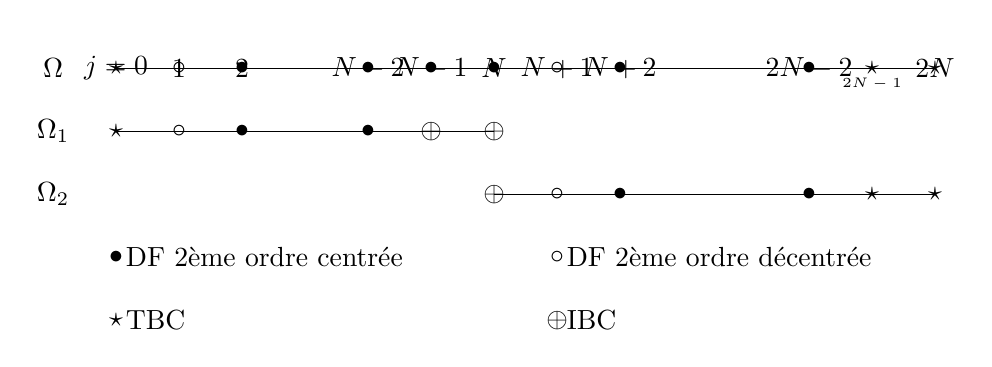
\begin{tikzpicture}[scale = .8]
	\coordinate (Alabel) at (-1,3);
	\coordinate (Aa) at (0,3);
	\coordinate (Ab) at (1,3);
	\coordinate (Ac) at (2,3);
	\coordinate (Ad) at (4,3);	
	\coordinate (Ae) at (5,3);	
	\coordinate (Af) at (6,3);	
	\coordinate (Ag) at (7,3);	
	\coordinate (Ah) at (8,3);	
	\coordinate (Ai) at (11,3);
	\coordinate (Aj) at (12,3);
	\coordinate (Ak) at (13,3);
	
	\draw (Aa) -- (Ak);
	\draw (Alabel) node {$\Omega$}; 
	\draw (Aa) node[label] {$j=0$};
	\draw (Ab) node[label] {$1$};
	\draw (Ac) node[label] {$2$};
	\draw (Ad) node[label] {$N-2$};
	\draw (Ae) node[label] {$N-1$};
	\draw (Af) node[label] {$N$};
	\draw (Ag) node[label] {$N+1$};
	\draw (Ah) node[label] {$N+2$};
	\draw (Ai) node[label] {$2N-2$};
	\draw (Aj) node[below,font=\tiny] {$2N-1$};
	\draw (Ak) node[label] {$2N$};
		
	\draw (Aa) node {$\star$};
	\draw (Ab) node {$\circ$};
	\draw (Aj) node {$\star$};
	\draw (Ak) node {$\star$};
	
	\draw (Ac) node{$\bullet$};
	\draw (Ad) node {$\bullet$};
	\draw (Ae) node {$\bullet$};
	\draw (Af) node{$\bullet$};	
	\draw (Ag) node{$\circ$};
	\draw (Ah) node {$\bullet$};
	\draw (Ai) node {$\bullet$};


	\coordinate (Blabel) at (-1,2);	
	\coordinate (Ba) at (0,2);
	\coordinate (Bb) at (1,2);
	\coordinate (Bc) at (2,2);
	\coordinate (Bd) at (4,2);	
	\coordinate (Be) at (5,2);	
	\coordinate (Bf) at (6,2);	

	\draw (Ba) -- (Bf); 
	
	\draw (Blabel) node {$\Omega_1$}; 
	\draw (Ba) node {$\star$};
	\draw (Bb) node {$\circ$};
	
	\draw (Bc) node {$\bullet$};
	\draw (Bd) node {$\bullet$};
	
	\draw (Be) node {$\oplus$};
	\draw (Bf) node {$\oplus$};	
	
	\coordinate (Clabel) at (-1,1);	
	\coordinate (Cf) at (6,1);	
	\coordinate (Cg) at (7,1);	
	\coordinate (Ch) at (8,1);	
	\coordinate (Ci) at (11,1);
	\coordinate (Cj) at (12,1);
	\coordinate (Ck) at (13,1);
		
	\draw (Cf) -- (Ck); 
	\draw (Clabel) node {$\Omega_2$}; 
	\draw (Cf) node{$\oplus$};
	\draw (Cg) node{$\circ$};
	\draw (Ch) node{$\bullet$};	
	\draw (Ci) node{$\bullet$};	
	\draw (Cj) node {$\star$};
	\draw (Ck) node{$\star$};
	
	%% Legend
	\draw (0,0) node {$\bullet$} node[right] {DF 2ème ordre centrée};
	\draw (7,0) node {$\circ$} node[right] {DF 2ème ordre décentrée};
	\draw (0,-1) node {$\star$} node[right] {TBC};
    \draw (7,-1) node {$\oplus$} node[right] {IBC};
	
\end{tikzpicture}
\captionof{figure}{Schéma indiquant la discrétisation spatiale imposée pour chaque point du monodomaine et des subdomaines de la DDM \label{fig:discretizations}}
\endgroup


\subsubsection{Vérification numérique de l'erreur due aux TBCs approximées}

\indent Le problème \eqref{eq:problemDDM1} - \eqref{eq:problemDDM2} a été résolu jusqu'à convergence avec cinq discrétisations spatiales uniformes différentes, au long d'un pas de temps (dans l'intervale $[0,\Delta t]$). Dans chaque cas, la solution de référence $u^{ref}$ était la solution au problème du monodomaine \eqref{eq:problemMonodomain}, résolu avec la même taille de maille. Deux erreurs ont été calculées :

\begin{equation*}
	e^{N,*} = |u^{ref}_N - u^{*}_N|
\end{equation*}

\begin{equation}
	\label{eq:errorDDM}
	e^{\Omega,*} = ||u^{ref}_N - u^{*}_N||_2 = \sqrt{\Delta x \left[ \sum_{j=0}^N{(u^{ref}_j - u^{1,\infty}_j)^2 } + \sum_{j=N}^{2N}{(u^{ref}_j - u^{2,\infty}_j)^2 } \right] }
\end{equation}

\noindent correspondant respectivement à l'erreur sur l'interface et à l'erreur dans tout le domaine.

\indent On s'intéresse au comportement de ces erreurs en fonction de la taille de maille. Comme le montre la figure \ref{fig:orderVerification}, on vérifie que la DDM proposée par nous, utilisant les TBCs approximées \eqref{eq:appTBCP0}, produit une erreur d'ordre $\mathcal{O}(\Delta x)$  :

\begingroup
\begin{center}
	\includegraphics[scale=.5]{figures/convergenceVerificationCorrectN.png}
	\captionof{figure}{Vérification numérique de l'ordre de convergence de l'erreur due à la DDM \label{fig:orderVerification}}
\end{center}
\endgroup

\subsubsection{Corrections pour les TBCs approximées}

\indent On propose des modifications pour les TBCs utilisées dans l'ASM afin d'annuler ces erreurs :

\begin{equation}
	\label{eq:TBCs_corriges}
    \begin{gathered}
        \Theta_1^{c_L}(u_2^{n+1,k+1}) + \theta_1 = \Theta_1^{c_L}(u_1^{n+1,k}) + \theta_1' \\
        \Theta_2^{c_R}(u_1^{n+1,k+1}) + \theta_2 = \Theta_2^{c_R}(u_2^{n+1,k}) + \theta_2' \\
        \Theta_3^{c_R}(u_1^{n+1,k+1}) + \theta_3 = \Theta_3^{c_R}(u_2^{n+1,k}) + \theta_3'
    \end{gathered}
\end{equation}

\noindent avec $\theta_i, \theta_i'$  donnés par 

\begin{gather*}
    \theta_1 = \Delta x c_L \frac{u_{N+1}^2 - 2u_{N}^2 + u_{N-1}^1}{\Delta x^2} + c_L^2\frac{\Delta x}{\Delta t} \left( u_{N}^2 - \alpha_{N}^2 \right)\\
    \theta_1' = - c_L^2\frac{\Delta x}{\Delta t} \left( u_{N}^1 - \alpha_{N}^1 \right)
\end{gather*}

\begin{equation*}
\begin{gathered}
    \theta_2 = \frac{\Delta x}{\Delta t} c_R^2 (u_N^1 - \alpha_N^1) \\
    \theta_2' = -\frac{\Delta x}{\Delta t} c_R^2 (u_N^2 - \alpha_N^2)
\end{gathered}
\end{equation*}

\begin{equation*}
\begin{gathered}
    \theta_3 = 2\frac{\Delta x}{\Delta t} \left[-\Delta x(u_{N-1}^1 - \alpha_{N-1}^1) - c_R (u_N^1 - \alpha_N^1) \right] + \Delta x \frac{u_{N-3}^1 - 2u_{N-2}^1 + u_{N-1}^1}{\Delta x^2} \\
    \theta_3' = 0
\end{gathered}
\end{equation*}

\indent On peut facilement vérifier que, à convergence, les TBCs corrigées \eqref{eq:TBCs_corriges} ramènent à l'expression \eqref{eq:FDdiscretization} écrite pour les points $x_N \in \Omega_2$, $x_N \in \Omega_1 $ et $x_{N-1} \in \Omega_1$, respectivement. 

%\indent En fait, on a, dans la convergence de la première condition à l'interface :
%
%\begin{equation*}
%\label{eq:modifiedTBC1}
%\begin{aligned}
%&& &    \Theta_1^{c_L}(u_N^*) + \theta_1 = \Theta_1^{c_L}(u_N^*) + \theta_1' \\
%&& \implies &    u_N^* - c_L \frac{u_{N+1}^* - u_N^*}{\Delta x} + c_L^2\frac{u_N^* - 2u_{N+1}^* + u_{N+2}^*}{\Delta x^2} + \\ 
%&& & \Delta x c_L \frac{u_{N+1}^* - 2u_{N}^* + u_{N-1}^*}{\Delta x^2} + c_L^2\frac{\Delta x}{\Delta t} \left( u_{N}^* - \alpha_{N}^* \right) = \\
%&& & u_N^* - c_L \frac{u_{N}^* - u_{N-1}^*}{\Delta x} + c_L^2\frac{u_N^* - 2u_{N-1}^* + u_{N-2}^*}{\Delta x^2}  - c_L^2\frac{\Delta x}{\Delta t} \left( u_{N}^* - \alpha_{N}^* \right) \\
% && \implies &    2c_L^2 \frac{-\frac{1}{2}u_{N-2}^* + u_{N-1}^* - u_{N+1}^* + \frac{1}{2}u_{N+2}^* }{\Delta x ^2}  +             2c_L^2\frac{\Delta x}{\Delta t} \left( u_{N}^* - \alpha_{N}^* \right) = 0  \\
%&& \implies &    \frac{u_{N}^* - \alpha_{N}^*}{\Delta t} + \frac{-\frac{1}{2}u_{N-2}^* + u_{N-1}^* - u_{N+1}^* + \frac{1}{2}u_{N+2}^* }{\Delta x ^3} = 0
%\end{aligned}
%\end{equation*}
%
%\indent ce qui est identique à \eqref{eq:FDdiscretization} satisfaite dans $x_N$.
%
%\indent Pour la deuxième IBC : 
%
%\begin{equation}
%\label{eq:modifiedTBC2}
%\begin{aligned}
%&& &\Theta_2^{c_R}(u_N^*) + \theta_2 = \Theta_2^{c_R}(u_N^*) + \theta_2'  \\
%&& \implies & u_N^* - c_R^2 \frac{u_N^* - 2u_{N-1}^* + u_{N-2}^*}{\Delta x^2} + \frac{\Delta x}{\Delta t} c_R^2 (u_N^* - \alpha_N^*)  = \\ && & u_N^* - c_R^2 \frac{u_N^* - 2u_{N+1}^* + u_{N+2}^*}{\Delta x^2} -\frac{\Delta x}{\Delta t} c_R^2 (u_N^* - \alpha_N^*)  \\
%&& \implies & 2\frac{\Delta x}{\Delta t} c_R^2 (u_N^* - \alpha_N^*) + 2c_R^2 \frac{-\frac{1}{2}u_{N-2}^* + u_{N-1}^* - u_{N+1}^* + \frac{1}{2}u_{N+2}^* }{\Delta x^2} = 0   \\
%&& \implies &\frac{u_N^* - \alpha_N^*}{\Delta t} + \frac{-\frac{1}{2}u_{N-2}^* + u_{N-1}^* - u_{N+1}^* + \frac{1}{2}u_{N+2}^* }{\Delta x^3} = 0
%\end{aligned}
%\end{equation}
%
%\noindent ce qui correspond également à \eqref{eq:FDdiscretization} satisfait dans $x_N$.
%
%\indent Finalement, pour la troisième IBC, on utilise \eqref{eq:modifiedTBC2} dans \eqref{eq:TBCsIterOmega1B} pour obtenir
%
%\begin{equation*}
%-\frac{u_{N-1}^* - 2 u_{N}^* + u_{N+1}^*}{\Delta x} + 2c_R\Delta x\frac{u_N^* - \alpha_N^*}{\Delta t} = 0 
%\end{equation*}
%
%\indent Ainsi
%
%\begingroup
%\begin{align*}
%\label{eq:modifiedTBC3}
%&&  &\Theta_3^{c_R}(u_N^*) + \theta_3 = \Theta_3^{c_R}(u_N^*) + \theta_3'    \\
%&& \implies & \frac{u_N^* - u_{N-1}^*}{\Delta x} + c_R \frac{u_N^* - 2u_{N-1}^* + u_{N-2}^*}{\Delta x^2} + 2\frac{\Delta x}{\Delta t}  \left[-\Delta x(u_{N-1}^* - \alpha_{N-1}^*) - c_R (u_N^* - \alpha_N^*) \right] + \\
%&&   & 			\frac{u_{N-3}^* - 2u_{N-2}^* + u_{N-1}^*}{\Delta x}  =  \frac{u_{N+1}^* - u_{N}^*}{\Delta x} + c_R \frac{u_N^* - 2u_{N+1}^* + u_{N+2}^*}{\Delta x^2} \\
%&&  \implies &  -\frac{u_{N-1}^* - 2 u_{N}^* + u_{N+1}^*}{\Delta x} + 2c_R\Delta_x\frac{u_N^* - \alpha_N^*}{\Delta t} + \\
%&&   & 2\frac{\Delta x}{\Delta t} \left[-\Delta x(u_{N-1}^* - \alpha_{N-1}^*) - c_R(u_N^* - \alpha_N^*) \right] + \frac{u_{N-3}^* - 2u_{N-2}^* + u_{N-1}^*}{\Delta x} = 0 \\
%&& \implies  & -2\frac{-\frac{1}{2}u_{N-3}^* + u_{N-2}^* - u_{N}^* + \frac{1}{2}u_{N+1}^* }{\Delta x} - 2\frac{\Delta x^2}{\Delta t}(u_{N-1}^* - 					\alpha_{N-1}^*) = 0 \\
%&& \implies &  \frac{u_{N-1}^* - \alpha_{N-1}^*}{\Delta t} + \frac{-\frac{1}{2}u_{N-3}^* + u_{N-2}^* - u_{N}^* + \frac{1}{2}u_{N+1}^* }{\Delta x ^3} = 0
%\end{align*}
%\endgroup
%
%\noindent ce qui est la discrétisation \eqref{eq:FDdiscretization} écrite pour le point $x_{N-1}$.

% 12/09/2016
\subsection{Optimisation des IBCs (vitesse de convergence)}

\indent Après la proposition et validation de la DDM avec des IBCs corrigées, notre neuf objectif maintenant était d'optimiser ces IBCs, afin de minimiser le nombre de itérations de l'ASM pour arriver à la convergence. Ainsi, on a fait un très large ensemble de tests, afin de trouver les coefficients $c_L$ et $c_R$ qui fournissent la convergence la plus rapide. Dans un premier temps, on a fait cette étude avec un pas temporel et un pas spatial fixés, afin d'analyser exclusivement l'influence du coefficient; ensuite, on a introduit ces deux paramètres dans l'étude.

\indent Comme on connaît une solution de référence, le critère de convergence utilisé est

\begin{equation*}
\label{eq:criteriaConvergence}
	e^{\Omega,k} \leq \epsilon
\end{equation*}

\noindent avec $\epsilon = 10^{-9}$ et  l'erreur $e^{\Omega,k}$, pour chaque itération $k$, définie comme dans \eqref{eq:errorDDM}.

\indent Afin de simplifier les tests et d'éviter des coûts de calcul trop élevés,  on a considéré, à chaque fois, $c_L = c_R = c$  dans le procès d'optimisation. Le rang des coefficients testés est $[-10.0, 20.0]$ (choisi après des tests initiaux pour identifier un intervalle approprié), avec un pas égal à  $0.1$ entre eux (ou encore plus petit, jusqu'à $0.005$, dans les régions les plus proches des coefficients optimaux, afin de raffiner la recherche). Le nombre maximal d'itérations est 100.

\indent Comme une dernière remarque, on rappelle que tous les tests ont été réalisés au long d'un seul pas de temps.

\subsubsection{Tests variant l'instant initial et la position de l'interface}

\indent On a utilisé un pas de temps $\Delta t = 20/2560 = 0.0078125$ et une taille de maille $\Delta x = 12/500 = 0.024$ fixés. Par ailleurs, on a mis en place deux ensembles de tests, nous permettant d'étudier la vitesse de convergence avec des différentes conditions initiales et différentes tailles des subdomaines :

\begin{enumerate}
	\item Tests variant l'instant initial $t_0$, avec l'interface fixée sur le centre du monodomaine $\Omega = [-6,6]$;
	\item Tests variant la position de l'interface ($x_{interface} = -L + \alpha 2L$, où  $L = 6$ et $0 < \alpha < 1$), pour un instant initial $t_0 = 0.78125$ fixé.
\end{enumerate}

\indent Dans tous les cas, la solution de référence $u^{ref}$ est la solution au problème dans le monodomaine \eqref{eq:problemMonodomain}, calculée dans $[t_0,t_0 + \Delta t]$.

\indent Les résultats obtenus sont résumés dans les figures \ref{fig:optimVarT0} et \ref{fig:optimVarInterface}, avec le nombre d'itérations pour arriver à la convergence en fonction du coefficient $c$. Par souci de clarté, les résultats pour les coefficients négatifs et positifs sont présentés dans des graphes séparés. Ils montrent des comportements très similaires pour toutes les courbes, avec deux minima for $c < 0$ et deux autres for $c > 0$, avec approximativement la même valeur dans tous les cas (environ -1.35, -0.10, 0.20 et 4.50). Les minima les plus proches de zéro sont associés à des courbes très discontinues, tandis que les deux deux minima sont associés à des courbes plus lisses (voir les détails dans les figures \ref{fig:optimVarT0NDetail}-\ref{fig:optimVarT0PDetail2} et \ref{fig:optimVarInterfaceNDetail}-\ref{fig:optimVarInterfacePDetail2}). Finalement, on remarque que, pour quelques courbes, le minimum est associé aux coefficients les plus proches de zéro, et pour les autres courbes, il est associée aux autres coefficients. Néanmoins, dans tous ces cas, les nombres optimaux d'itérations sont similaires (entre cinq et sept).

\begingroup
\noindent
\begin{minipage}[t]{.45\linewidth}
	\includegraphics[scale=.4]{figures/FinalFigures/NiterxCoefVarT0FinalVersionN.png}
	\captionof{subfigure}{Vue générale des coefficients négatifs}
\end{minipage}
\hfill
\begin{minipage}[t]{.45\linewidth}
	\includegraphics[scale=.4]{figures/FinalFigures/NiterxCoefVarT0FinalVersionP.png}
	\captionof{subfigure}{Vue générale des coefficients positifs}
\end{minipage}
\begin{minipage}[t]{.45\linewidth}
	\includegraphics[scale=.4]{figures/FinalFigures/NiterxCoefVarT0FinalVersionNDetail.png}
	\captionof{subfigure}{Détail autour d'un des coefficients optimaux négatifs  \label{fig:optimVarT0NDetail}}
\end{minipage}
\hfill
\begin{minipage}[t]{.45\linewidth}
	\includegraphics[scale=.4]{figures/FinalFigures/NiterxCoefVarT0FinalVersionNDetail2.png}
	\captionof{subfigure}{Détail autour de l'autre coefficient optimal négatif  \label{fig:optimVarT0NDetail2}}
\end{minipage}
\begin{minipage}[t]{.45\linewidth}
	\includegraphics[scale=.4]{figures/FinalFigures/NiterxCoefVarT0FinalVersionPDetail.png}
	\captionof{subfigure}{Détail autour d'un des coefficients optimaux positifs \label{fig:optimVarT0PDetail} }
\end{minipage}
\hfill
\begin{minipage}[t]{.45\linewidth}
	\includegraphics[scale=.4]{figures/FinalFigures/NiterxCoefVarT0FinalVersionPDetail2.png}
	\captionof{subfigure}{Détail autour de l'autre coefficient optimal positif   \label{fig:optimVarT0PDetail2}}
\end{minipage}
	\captionof{figure}{Nombre d'itérations jusqu'à convergence en fonction du coefficient des TBCs, pour une interface fixée et différentes valeurs de $t_0$  \label{fig:optimVarT0}}
\endgroup

\begingroup
\noindent
\begin{minipage}{.45\linewidth}
	\includegraphics[scale=.4]{figures/FinalFigures/NiterxCoefVarInterfaceFinalVersionN.png}
	\captionof{subfigure}{Vue générale des coefficients négatifs}
\end{minipage}
\hfill
\begin{minipage}{.45\linewidth}
	\includegraphics[scale=.4]{figures/FinalFigures/NiterxCoefVarInterfaceFinalVersionP.png}
	\captionof{subfigure}{Vue générale des coefficients positifs}
\end{minipage}
\begin{minipage}{.45\linewidth}
	\includegraphics[scale=.4]{figures/FinalFigures/NiterxCoefVarInterfaceFinalVersionNDetail.png}
	\captionof{subfigure}{Détail autour d'un des coefficients optimaux négatifs  \label{fig:optimVarInterfaceNDetail}}
\end{minipage}
\hfill
\begin{minipage}{.45\linewidth}
	\includegraphics[scale=.4]{figures/FinalFigures/NiterxCoefVarInterfaceFinalVersionNDetail2.png}
	\captionof{subfigure}{Détail autour de l'autre coefficient optimal négatif  \label{fig:optimVarInterfaceNDetail2}}
\end{minipage}
\begin{minipage}{.45\linewidth}
	\includegraphics[scale=.4]{figures/FinalFigures/NiterxCoefVarInterfaceFinalVersionPDetail.png}
	\captionof{subfigure}{Détail autour d'un des coefficients optimaux positifs \label{fig:optimVarInterfacePDetail}  }
\end{minipage}
\hfill
\begin{minipage}{.45\linewidth}
	\includegraphics[scale=.4]{figures/FinalFigures/NiterxCoefVarInterfaceFinalVersionPDetail2.png}
	\captionof{subfigure}{Détail autour de l'autre coefficient optimal positif  \label{fig:optimVarInterfacePDetail2}}
\end{minipage}
	\captionof{figure}{Nombre d'itérations jusqu'à convergence en fonction du coefficient des TBCs, pour $t_0$ fixé et différentes positions de l'interface \label{fig:optimVarInterface}}
\endgroup

\indent

\indent La figure \ref{fig:errorEvolution} montre l'évolution de l'erreur, en fonction des itérations, pour les cinq coefficients $c$ qui ont fournit les convergences les plus rapides, pour un temps initial et une position de l'interface fixés. Pour d'autres valeurs de $t_0$ et $\alpha$, le graphe est similaire, en ce qui concerne le nombre d'itérations et le fait que la convergence est plus régulière pour les coefficients les plus proches de zéro, en comparaison aux autres coefficients optimaux.

\begin{figure}
\begin{center}
\includegraphics[scale=.5]{figures/FinalFigures/errorEvolutionFixedT0BFinalVersion.png}
\caption{Évolution de l'erreur, en fonction des itérations, pour les tests les plus rapides \label{fig:errorEvolution}}
\end{center}
\end{figure}

\subsubsection{Tests variant $\Delta t$ and $\Delta x$}

\indent Après avoir vérifié que la méthode se comporte de façon similaire pour toute condition initiale (i.e., pour tout $t_0$) et toute position de l'interface, on a fixé ces paramètres ($t_0 = 0$ and $\alpha = 0.5$) et on a fait de nouveaux tests avec différentes valeurs de $\Delta t$ (avec $\Delta x = 12/250$ fixé) et différentes valeurs de $\Delta x$ (avec $\Delta t = 0.02$ fixé).

\indent Le nombre d'itérations en fonction des coefficients, pour certains tests, est présenté dans les figures \ref{fig:niterxCoefVarDt} et \ref{fig:niterxCoefVarDx}. La figure \ref{fig:optimalCoefVarDxDtCorrectN} présente le coefficient optimal pour chaque $\Delta t$ ou $\Delta x$. En considérant la remarque qu'on a faite concernant les résultats similaires (i.e., le nombre d'itérations jusqu'à convergence) pour les quatre coefficients optimaux, on a seulement tenu compte, pour la construction des courbes de la figure \ref{fig:optimalCoefVarDxDtCorrectN}, les minima les plus éloignés de zéro: comme le montre les figures \ref{fig:niterxCoefVarDt} et \ref{fig:niterxCoefVarDx}, ces minima ont une forte dépendance de $\Delta t$ et $\Delta x$, et on cherchait à étudier cette relation.

\begingroup
\noindent
\begin{minipage}{.45\linewidth}
	\includegraphics[scale=.45]{figures/FinalFigures/NiterxCoefVarDtdx250FinalVersionNMarshal.png}
\captionof{subfigure}{Coefficients négatifs}
\end{minipage}
\hfill
\begin{minipage}{.45\linewidth}
	\includegraphics[scale=.45]{figures/FinalFigures/NiterxCoefVarDtdx250FinalVersionPMarshal.png}
\captionof{subfigure}{Coefficients positifs}
\end{minipage}
\captionof{figure}{Nombre d'itérations jusqu'à convergence en fonction du coefficient pour $2N = 250$ fixé et des différentes valeurs de $\Delta t$  \label{fig:niterxCoefVarDt}}
\endgroup

\begingroup
\noindent \begin{minipage}{.45\linewidth}
	\includegraphics[scale=.45]{figures/FinalFigures/NiterxCoefVarDxdt2em2FinalVersionN.png}
\captionof{subfigure}{Negative coefficients}
\end{minipage}
\hfill
\begin{minipage}{.45\linewidth}
	\includegraphics[scale=.45]{figures/FinalFigures/NiterxCoefVarDxdt2em2FinalVersionP.png}
\captionof{subfigure}{Positive coefficients}
\end{minipage}
\captionof{figure}{Nombre d'itérations jusqu'à convergence en fonction du coefficient des TBCspour $\Delta t = 0.02$ et des différentes valeurs de $\Delta x$  \label{fig:niterxCoefVarDx}}
\endgroup


\begin{center}
	\includegraphics[scale=.5]{{figures/FinalFigures/OptimalCoefVarDxDtFinalVersionMarshal.png}}
	\captionof{figure}{Coefficients optimaux en fonction du pas de temps et de la taille de maille\label{fig:optimalCoefVarDxDtCorrectN}}
\end{center}

\indent La figure \ref{fig:optimalCoefVarDxDtCorrectN} suggère que le coefficient optimal dépende de $(\Delta t)^\nu$ et $(\Delta x)^\eta$, avec $0 \leq \nu \leq 1$ et $\eta < 0$. En fait, en faisant quelques régressions avec $\Delta t $ ou $\Delta x$ fixé, on peut conclure que $\nu = 2/3$ et $\eta = -1$ fournissent des courbes de régression très bien adaptées (avec des coefficients de détermination $R^2$ plus grandes que 0.99), pour les cas des coefficients positifs et négatifs (même que chacun de ces cas corresponde à des courbes différentes). Ainsi, on va chercher à modéliser une fonction de la forme

\begin{equation}
	\label{eq:regression2D}
	c_{opt}(\Delta t, \Delta x) = \kappa + \alpha (\Delta t)^{\frac{2}{3}} + \beta \frac{1}{\Delta x} + \gamma   \frac{(\Delta t)^{\frac{2}{3}}}{\Delta x}
\end{equation}

\indent Une régression utilisant les coins du rectangle $[0.001,0.1]\times[12/100,12/1000]$ et quinze points à l'intérieur fournit les surfaces 

\begin{gather}
	c_{opt}^+(\Delta t, \Delta x) = 0.0775 -0.3353 (\Delta t)^{\frac{2}{3}} - 0.0012 \frac{1}{\Delta x} + 2.7407   \frac{(\Delta t)^{\frac{2}{3}}}{\Delta x} 	\label{eq:regression2DPos} \\
	c_{opt}^-(\Delta t, \Delta x) = -0.0583 -1.5024 (\Delta t)^{\frac{2}{3}} - 0.0006 \frac{1}{\Delta x} -0.7287  \frac{(\Delta t)^{\frac{2}{3}}}{\Delta x} 	\label{eq:regression2DNeg}
\end{gather}

\noindent respectivement pour les coefficients optimaux positifs et négatifs. Les coefficients de détermination de chaque régression son $R^{2,+} = 0.9999894$ et $R^{2,-} = 0.9998993$, ce qui indique une bonne représentation.

\indent Afin de valider les expressions \eqref{eq:regression2DPos} et \eqref{eq:regression2DNeg}, elles ont été utilisées pour calculer le coefficient optimal pour plusieurs points $(\Delta t, \Delta x)$, avec $\Delta t \in [0.0005,0.3]$ et $\Delta x \in \left[12/5000,12/50 \right]$. De plus, ces coefficients ont été utilisés dans la résolution du problème avec la DDM. Comme le montre la figure \ref{fig:regressionValidation}, pour la plupart des points dans le domaine considéré, le coefficient optimal calculé fournit une convergence rapide vers la solution du monodomaine, avec moins de 20 itérations (ou encore moins de 12 itérations), sur une large région du domaine).

\begingroup
\noindent
\begin{minipage}[t]{.45\linewidth}
	\includegraphics[scale=.45]{figures/FinalFigures/contourValidationN.png}
	\captionof{subfigure}{Coefficients négatifs}
\end{minipage}
\hfill
\begin{minipage}[t]{.45\linewidth}
	\includegraphics[scale=.45]{figures/FinalFigures/contourValidationP.png}
	\captionof{subfigure}{Coefficients positifs}
\end{minipage}
\captionof{figure}{Lignes de contour du nombre d'itérations jusqu'à convergence, en utilisant les coefficients optimaux $c_{opt}^+(\Delta t, \Delta x)$ obtenus à partir des régressions. \label{fig:regressionValidation}}.
\endgroup

\indent Les nombres d'itérations présentés dans la figure \ref{fig:regressionValidation} ne sont pas les plus petits qu'on est capable de trouver (cf. les figures \ref{fig:optimVarT0} jusqu'à \ref{fig:niterxCoefVarDx}), parce que les expressions \eqref{eq:regression2DPos} et \eqref{eq:regression2DNeg} sont des régressions construites à partir de coefficients optimaux obtenus parmi un ensemble discret de valeurs possibles. Néanmoins, elles donnent de très bonnes approximations pour le $c$ optimal pour chaque $(\Delta t, \Delta x)$, et ainsi on peut chercher dans une petite région autour du $c_{opt}$ calculé pour obtenir une convergence encore plus rapide.

\subsection{Conclusion partielle}
 
\indent Les résultats présentés dans cette section montrent que la méthode de décomposition de domaine proposée ici, consistant en une méthode de Schwarz additive avec nos TBCs approximées, est capable de fournir une convergence rapide vers la solution du problème résolu dans le monodomaine. Alors, on a atteint notre objectif de résoudre l'équation de dispersion dans un domaine fini divisé en deux subdomaines.

\indent Par ailleurs, les résultats des tests d'optimisation sont très satisfaisants en ce qui concerne une application plus générale de notre méthode. Premièrement, pour des discrétisations spatiales et temporales fixées, on a trouvé des coefficients optimaux indépendants de la solution initiale et de la taille des subdomaines (\emph{i.e.}, indépendamment de l'instant initial et de la position de l'interface).  Deuxièmement, on a obtenu de très bonnes courbes et surfaces de régression pour les coefficients optimaux en fonction de $\Delta t$ et $\Delta x$, ce qui nous permet d'appliquer le modèle avec une convergence rapide dans d'autres cadres numériques que ceux testés dans cette étude.

\bibliography{../may/biblio}
\end{document}
